% ****** Start of file aipsamp.tex ******
%
%   This file is part of the AIP files in the AIP distribution for REVTeX 4.
%   Version 4.1 of REVTeX, October 2009
%
%   Copyright (c) 2009 American Institute of Physics.
%
%   See the AIP README file for restrictions and more information.
%
% TeX'ing this file requires that you have AMS-LaTeX 2.0 installed
% as well as the rest of the prerequisites for REVTeX 4.1
% 
% It also requires running BibTeX. The commands are as follows:
%
%  1)  latex  aipsamp
%  2)  bibtex aipsamp
%  3)  latex  aipsamp
%  4)  latex  aipsamp
%
% Use this file as a source of example code for your aip document.
% Use the file aiptemplate.tex as a template for your document.
\documentclass[%
 aip,
% jmp,
% bmf,
% sd,
% rsi,
 amsmath,amssymb,
%draft,%
 preprint,%
%author-year,%
%author-numerical,%
% Conference Proceedings
]{revtex4-1}
\usepackage{booktabs, multirow} % for borders and merged ranges
\usepackage{soul}% for underlines
\usepackage[table]{xcolor} % for cell colors
\usepackage{changepage,threeparttable} % for wide tables
% If the table is too wide, replace \begin{table}[!htp]...\end{table} with
% \begin{adjustwidth}{-2.5 cm}{-2.5 cm}\centering\begin{threeparttable}[!htb]...\end{threeparttable}\end{adjustwidth}

\usepackage{graphicx}% Include figure files
\usepackage{dcolumn}% Align table columns on decimal point
\usepackage{bm}% bold math
%\usepackage[mathlines]{lineno}% Enable numbering of text and display math
%\linenumbers\relax % Commence numbering lines
\usepackage{hyperref}
\usepackage[utf8]{inputenc}
\usepackage[T1]{fontenc}
\usepackage{mathptmx}
\usepackage[version=4]{mhchem}
\usepackage{siunitx}
%\usepackage{pdflscape}
\DeclareSIUnit[number-unit-product = {}]
\molar{\,M}
\DeclareSIUnit[number-unit-product = {}]
\ppm{\,ppm}

%%%%LaTeX Aliases %%%%%%%%%%
\newcommand{\ca}{\ce{C_\alpha} }
\newcommand{\cb}{\ce{C_\beta} }
\newcommand{\cg}{\ce{C_\gamma} }
\newcommand{\cd}{\ce{C_\delta} }
\newcommand{\cep}{\ce{C_\epsilon} }
\newcommand{\cz}{\ce{C_\zeta} }


\renewcommand\thefigure{S\arabic{figure}}
\renewcommand\thetable{S\arabic{table}}

\usepackage{longtable}
\setlength{\LTcapwidth}{\textwidth} %Make Longtable captions full text width
\usepackage{rotating}

\begin{document}

%\preprint{AIP/123-QED}

\title[SI: The dominant activated state of KcsA]{ \large  Supplementary Information: Informing NMR experiments with molecular dynamics simulations to characterize the dominant activated state of KcsA}
% Force line breaks with \\


\author{Sergio Pérez-Conesa}
\thanks{These three authors contributed equally}
 \affiliation{KTH Royal Institute of Technology, Science for Life Laboratory, Stockholm, Sweden}%

\author{Eric G. Keeler}
\thanks{These three authors contributed equally}
\affiliation{Department of Chemistry, Columbia University, New York, New York 10027, United States}

\author{Dongyu Zhang}
\thanks{These three authors contributed equally}
\affiliation{Department of Chemistry, Columbia University, New York, New York 10027, United States}
\affiliation{Current Address: Plexxikon Inc., Berkeley, CA 94710, United States}

\author{Lucie Delemotte}
\thanks{Correspondance to: lucied@kth.se, aem5@columbia.edu }
\affiliation{KTH Royal Institute of Technology, Science for Life Laboratory, Stockholm, Sweden}

\author{Ann E. McDermott}
\thanks{Correspondance to: lucied@kth.se, aem5@columbia.edu }
\affiliation{Department of Chemistry, Columbia University, New York, New York 10027, United States}

\date{\today}% It is always \today, today,
             %  but any date may be explicitly specified

\maketitle

\section{Supplementary Figures}

\begin{figure*}[!htb]
	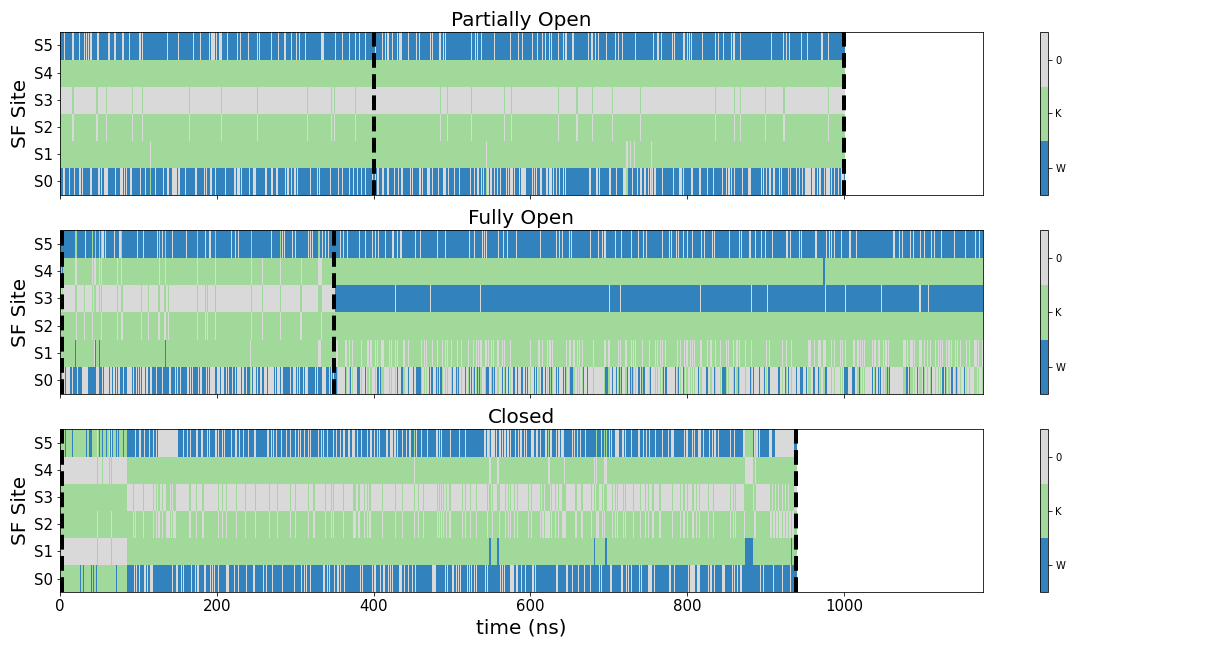
\includegraphics[width=\textwidth]{figures_SI/SF_occupation_print.png}
	 \caption{\scriptsize
	 Occupation of the canonical selectivity filter sites as a function of time in the MD simulations for the study states:  Partially Open (top), Fully Open (middle) and Closed (bottom). For the Fully Open state the simulation data from the entry of a water molecule in the S3 site is discarded since this has been identified as a pre-inactivation sign. 
}
\label{SI_SF_occupation}
\end{figure*}

\begin{figure*}[!htb]
	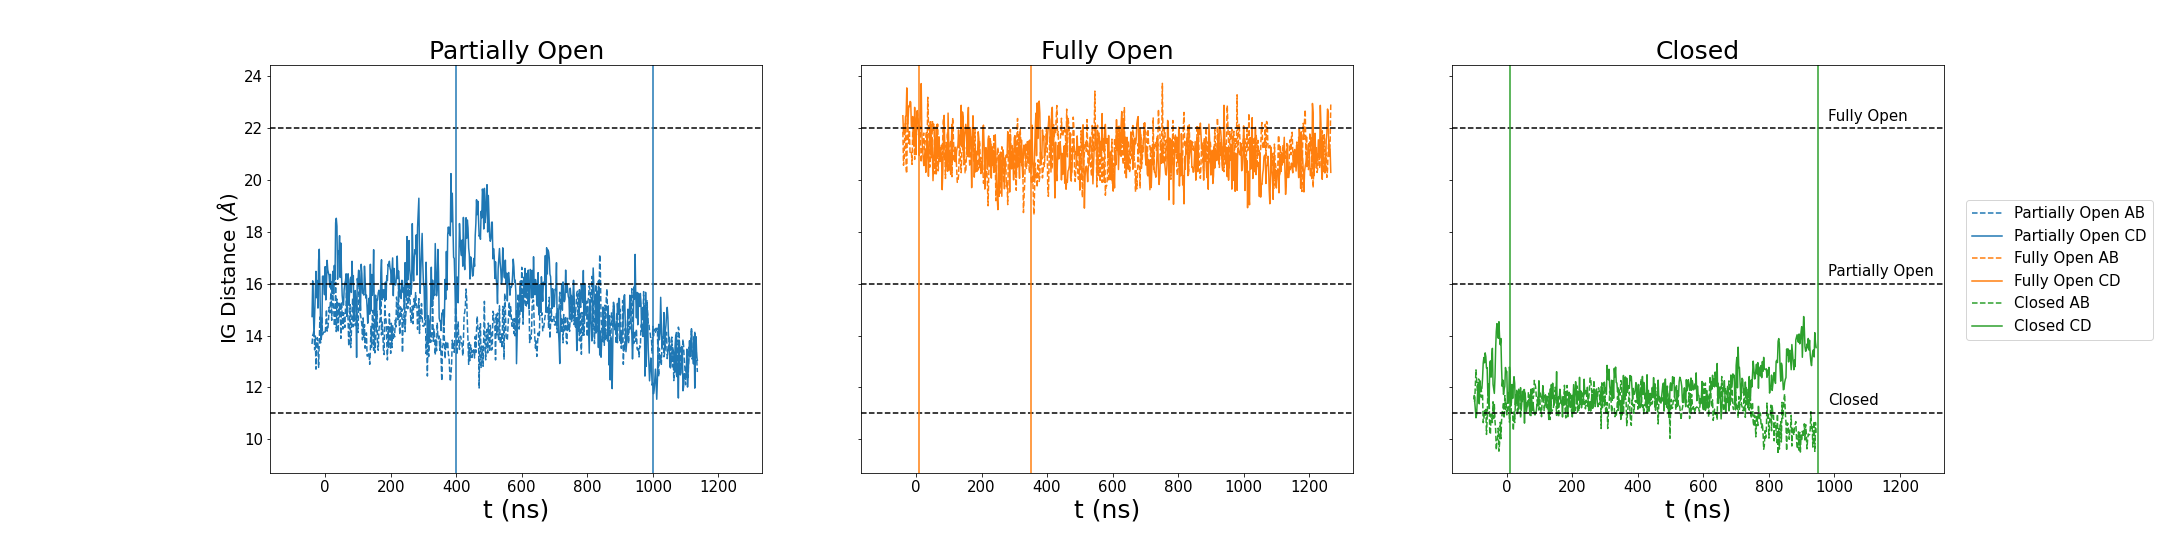
\includegraphics[width=\textwidth]{figures_SI/IG_print.png}
	 \caption{\scriptsize
	 Inner gate opening measured as the  T112 \ca distance of opposing subunits ( subunits AB solid line or subunits CD dashed line). Vertical lines delimit the part of the simulation analyzed. In the case of the partially open state the part with a more stable inner gate is used. For the Fully Open state this choice is based on selectivity filter occupation see Fig. \ref{SI_SF_occupation}. The data is smoothed with 50 point rolling median. Negative values of time are the equilibration period. }
\label{SI_IG}
\end{figure*} 

\begin{figure*}[!htb]
	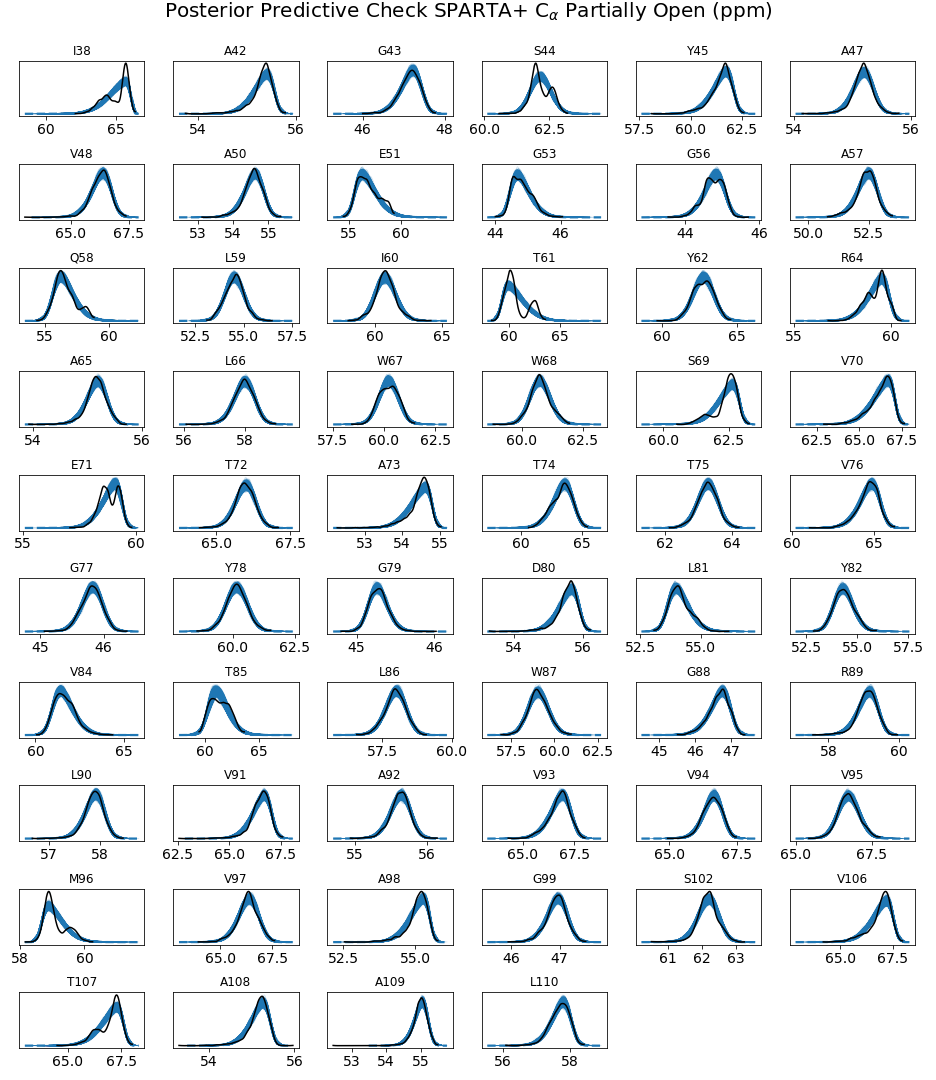
\includegraphics[width=\textwidth]{figures_SI/ppc_like_o_CA_sparta_plus.png}
	 \caption{\scriptsize
	 Posterior predictive checks for \ca chemical shift data of the different residues calculated for the Partially Open state simulation with the CS prediction method SPARTA+. A posterior predictive check consists in sampling the posterior probability distributions  ( for our case the posteriors of $\mu$, $\sigma$ and $\alpha$ parameters since the likelihood is a skew-gaussian distribution) to produce an ensemble of distributions (blue lines) that are compared to the data used for the inference (dashed black line). Similar posterior predictive checks have been obtained for the rest of states, methods and nuclei and can be found in \url{https://github.com/delemottelab/Informing_NMR_experiments_w_MD}
	 }
\label{SI_ppc}
\end{figure*}

\begin{figure*}[tbp]
	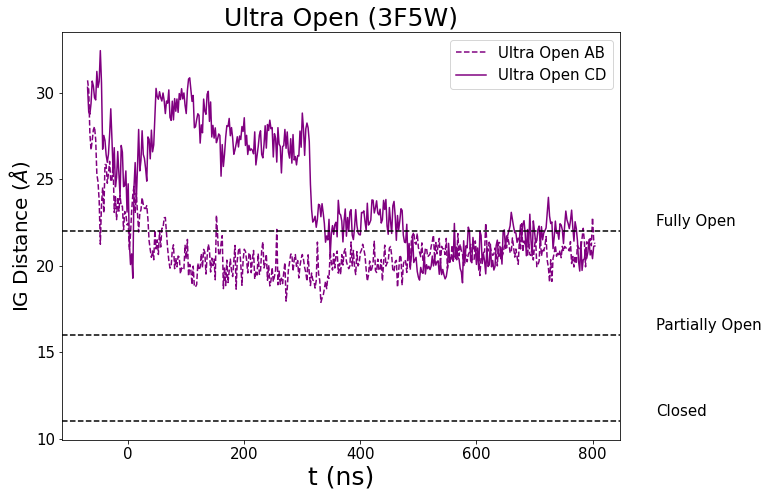
\includegraphics[width=0.65\textwidth]{figures_SI/IG_ultra_print.png}
	 \caption{\scriptsize
	 Inner gate opening measured as the  T112 \ca distance of opposing subunits ( subunits AB solid line or subunits CD dashed line) for the "Ultra Open" structure (PDB ID 3F5W). The structure is unstable and the inner gate rapidly decays to openings compatible with the Fully Open state (PDB ID 5VK6). For this reason this simulation was not analyzed in this work. }
\label{SI_IG_3F5W}
\end{figure*} 

\begin{figure*}[tbp]
	\includegraphics[width=\textwidth]{figures_SI/3D_SF_strip_plot_v2-01.eps}
	 \caption{\scriptsize
	 Representative strip plot of the 3D experiments NCACX (green), NCOCX (magenta), CANCO (cyan) collected at 900 MHz that were used for the backbone walk of assignments of KcsA in the activated state (3:1 DOPE:DOPG, 50 mM KCl, pH 4.0). The polarization pathway of the experiments is shown (top). The backbone walk for residues T74 to G79 is shown.
}
\label{SI_3D_strip_plot}
\end{figure*}

\begin{figure*}[tbp]
	\includegraphics[width=\textwidth]{figures_SI/Assignment_diagram_figure_v3-01.eps}
	 \caption{\scriptsize
	 Schematic indicating the assigned residues of KcsA in the activated state (3:1 DOPE:DOPG, 50 mM KCl, pH 4.0) with black filled in circles. The unassigned resonances are shown with gray filled circles. Open circles are used to indicate in which experiments the resonances are present. The 3D NCACX (green), NCOCX (magenta), and CANCO (cyan) and the 2D \ce{^13C}-\ce{^13C} DARR (purple) are shown, other assigned peaks are present in other experimental spectra that are not indicated on this figure (ZF-TEDOR (Pro), NcoCX, NcaCX, NCO, NCA). The resonances identified by statistical inference on the MD simulation data to be state markers are indicated with a red square and the agreement with the various states (Fully Open - orange, Partially Open - blue, Inconclusive - gray) are shown on the residue name and number. 
}
\label{SI_NMR_assign_scheme}
\end{figure*}

\begin{figure*}[tbp]
	\includegraphics[width=\textwidth]{figures_SI/2Ds_all_v2-01.eps}
	 \caption{\scriptsize
	 2D \ce{^13C}-\ce{^15N} NcaCX (a), NcoCX (b), and ZF-TEDOR (c) spectra of KcsA in the activated state (3:1 DOPE/DOPG, 50 mM KCl, pH 4.0) spectra collected at 900 MHz (a and b) and 750 MHz (c). Assigned resonances are labeled as either C$^i$-N$^i$ (NcaCX and ZF-TEDOR) or C$^{i-1}$-N$^i$ (NcoCX and ZF-TEDOR).
}
\label{SI_NMR_full_2Ds}
\end{figure*}

\begin{figure*}[tbp]
	\includegraphics[width=\textwidth]{figures_SI/exp_hist-05.eps}
	 \caption{\scriptsize
	 Histograms of the experimental difference ($\Delta\text{CS}_{\text{exp}} = \text{CS}_{\text{exp}}^{\text{pH=4,act}} - \text{CS}_{\text{exp}}^{\text{pH=7.5,deact}}$) between the activated and deactivated state assigned chemical shifts for (a) N, (b) \ca, (c) C, and (d) \cb. A fitted normal distribution is shown on each histogram (red lines) with the distribution equation and parameters shown, inset, demonstrating the proper referencing of the datasets to one another.
}
\label{SI_Exp_Hist}
\end{figure*}


\begin{figure*}[tbp]
	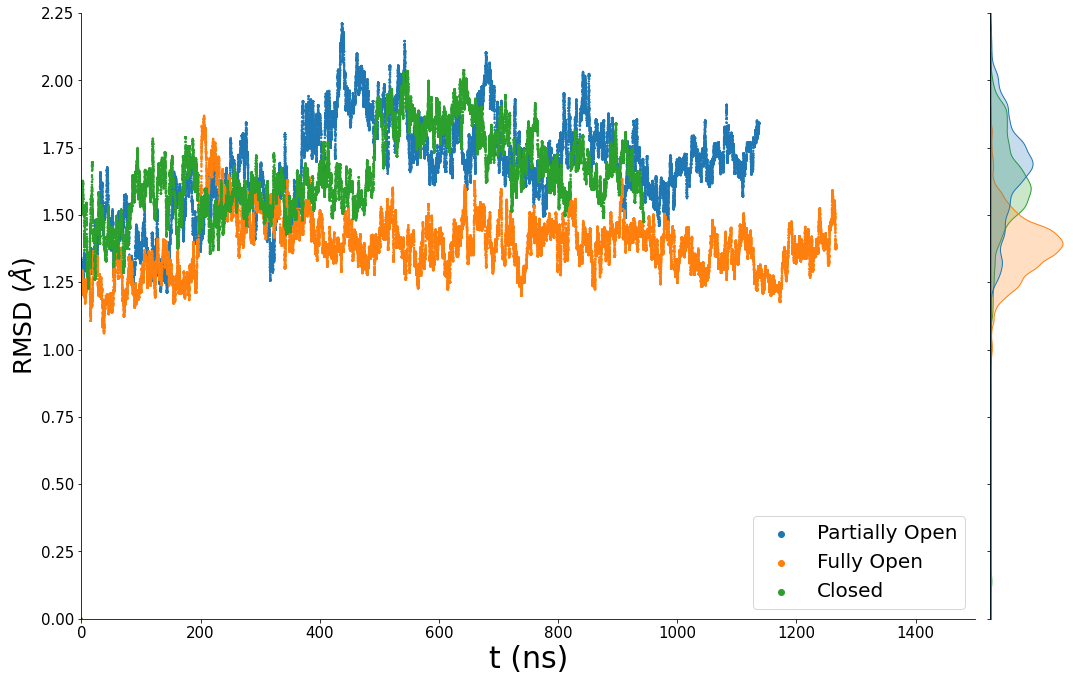
\includegraphics[width=\textwidth]{figures_SI/RMSD_print.png}
	 \caption{\scriptsize
	 Root mean square deviation (RMSD) of the \ca atom positions of the MD simulations as a function of time for the Partially Open, Fully Open and Closed states. Some of the noise is smoothed by a 10 step rolling median. Negative values of time are the equilibration period.
	 }
\label{SI_RMSD}
\end{figure*} 


\begin{figure*}[tbp]
	\includegraphics[width=\textwidth]{figures_SI/SHIFTX2_SPARTA-02.eps}
	 \caption{\scriptsize
	 Comparison of the predicted chemical shifts from the MD trajectories of the various states of KcsA using SPARTA+ and SHIFTX2. $\Delta\text{CS}_{\text{SPARTA+-SHIFTX2}} = \text{CS}^{\text{X}}_{\text{sim, SPARTA+}} - \text{CS}^{\text{X}}_{\text{sim, SHIFTX2}} $, where X is FO (orange), PO (blue), or Closed (green). The dashed lines represent a normal distribution fit to the histograms.
}
\label{SI_SPARTA_v_SHIFTX2}
\end{figure*}

\begin{sidewaysfigure}
	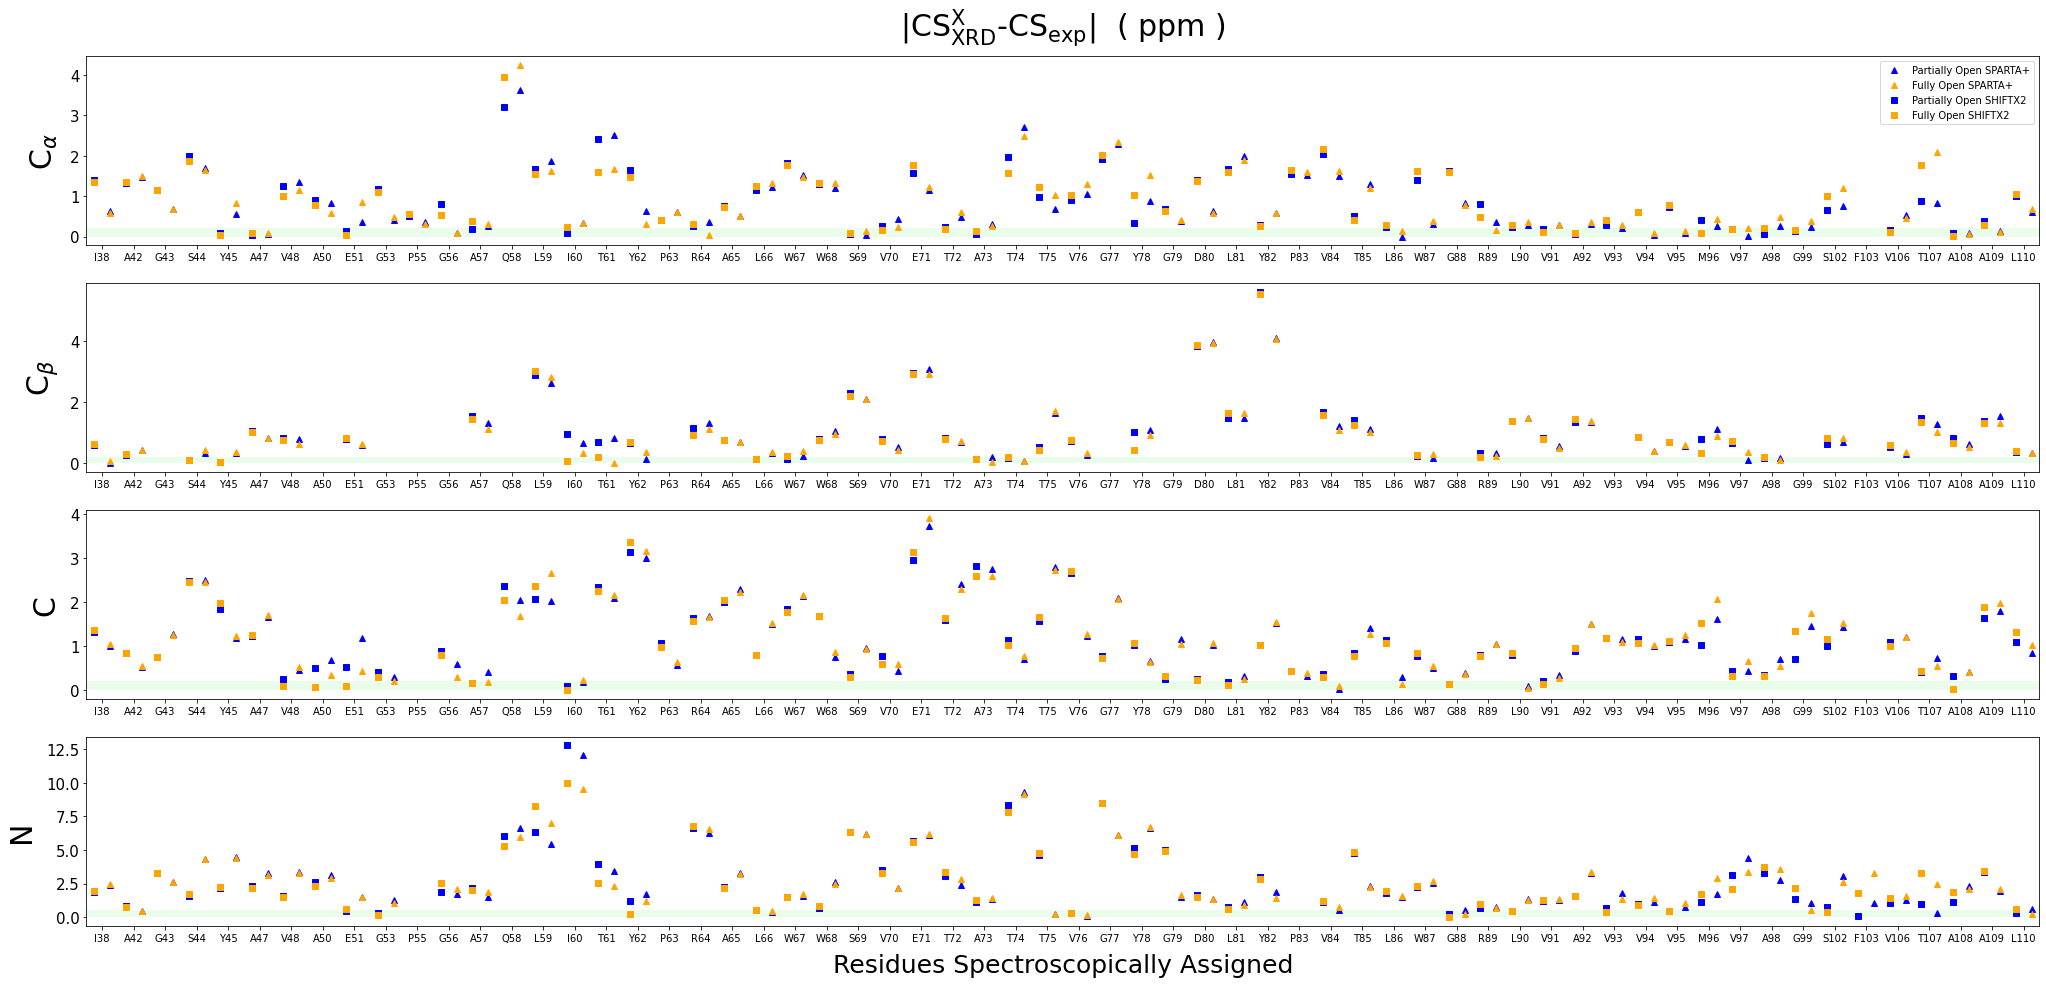
\includegraphics[width=\textwidth]{figures_SI/assignment_skew_model_all_print_no_ref_XRD.png}
 	 \caption{\scriptsize
    Chemical shifts difference between experiment and the calculated CS for the XRD structures ($\text{CS}_{\text{XRD}}^{\text{X}}-\text{CS}_{\text{exp}}$), where X represents the FO (orange) or PO (blue) sate. All residues on the x-axis for the different nuclei and chemical shift prediction methods. The agreement between the calculation and the NMR experiments is higher the closer the value is to zero. Chemical shifts predicted by SPARTA+ and SHIFTX2 are drawn with triangles and squares respectively. The green shade depicts the typical experimental uncertainty.}
\label{SI_assignment_XRD}
\end{sidewaysfigure}

\begin{figure*}[tbp]
	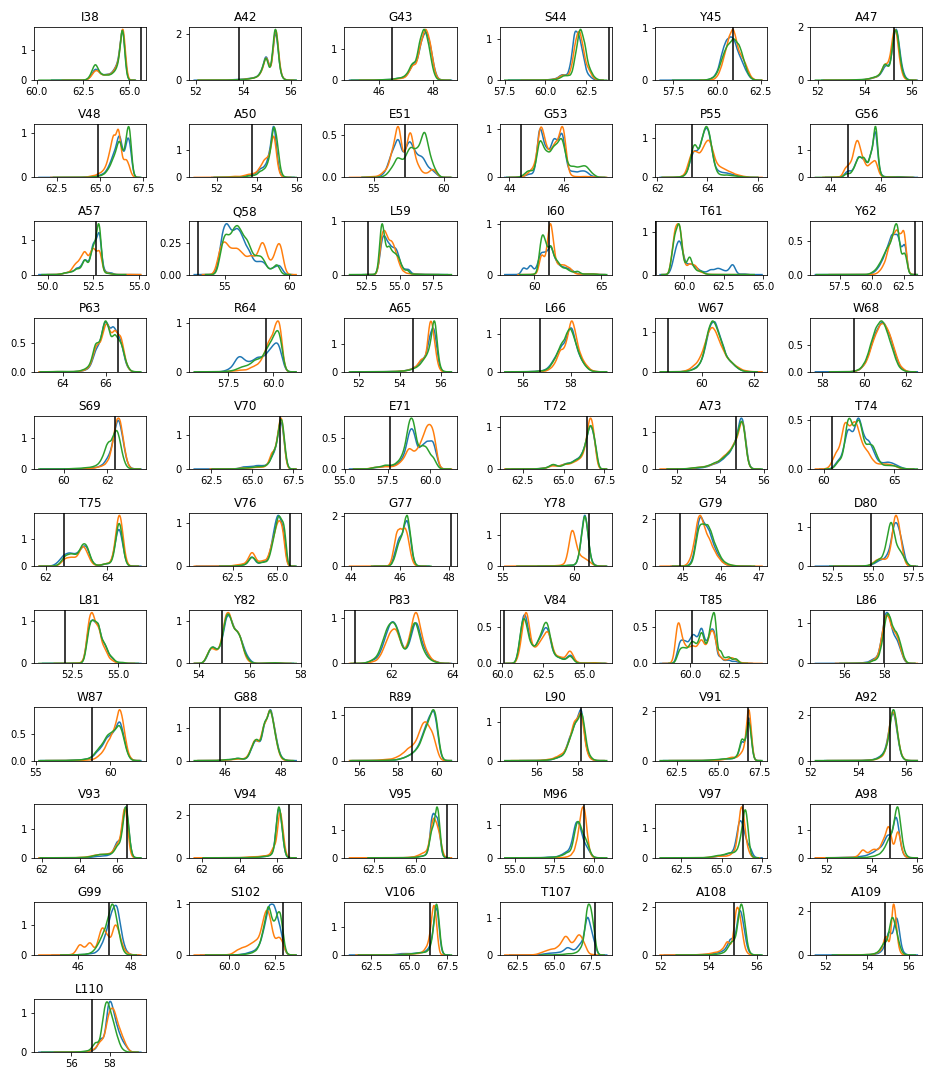
\includegraphics[width=\textwidth]{figures_SI/hist_shiftx2_CA.png}
	 \caption{\scriptsize
 Probability distributions of the raw simulated CS of the MD trajectory snapshots for the different residues assigned spectroscopically for the \ca nucleus and the CS prediction method SHIFTX2. Three different states are compared: Partially Open (blue), Fully Open (orange) and Closed (green). The vertical line indicates the NMR determined experimental CS for the activated state. The distributions are calculated using kernel density estimation as implemented in the python library Seaborn. 
}
\label{SI_hist1}
\end{figure*}

\begin{figure*}[tbp]
	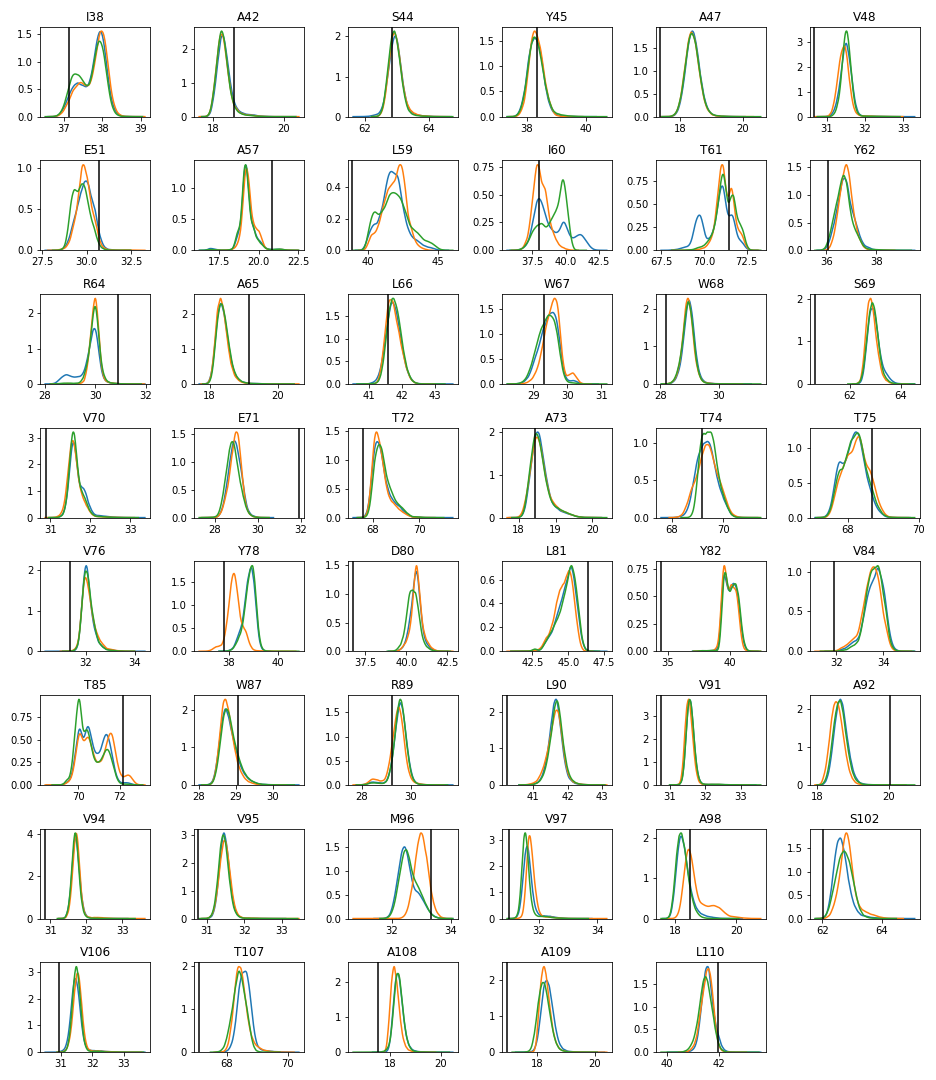
\includegraphics[width=\textwidth]{figures_SI/hist_shiftx2_CB.png}
	 \caption{\scriptsize
 Probability distributions of the raw simulated CS of the MD trajectory snapshots for the different residues assigned spectroscopically for the \cb nucleus and the CS prediction method SHIFTX2. Three different states are compared: Partially Open (blue), Fully Open (orange) and Closed (green). The vertical line indicates the NMR determined experimental CS for the activated state. The distributions are calculated using kernel density estimation as implemented in the python library Seaborn. 
}
\label{SI_hist2}
\end{figure*}

\begin{figure*}[tbp]
	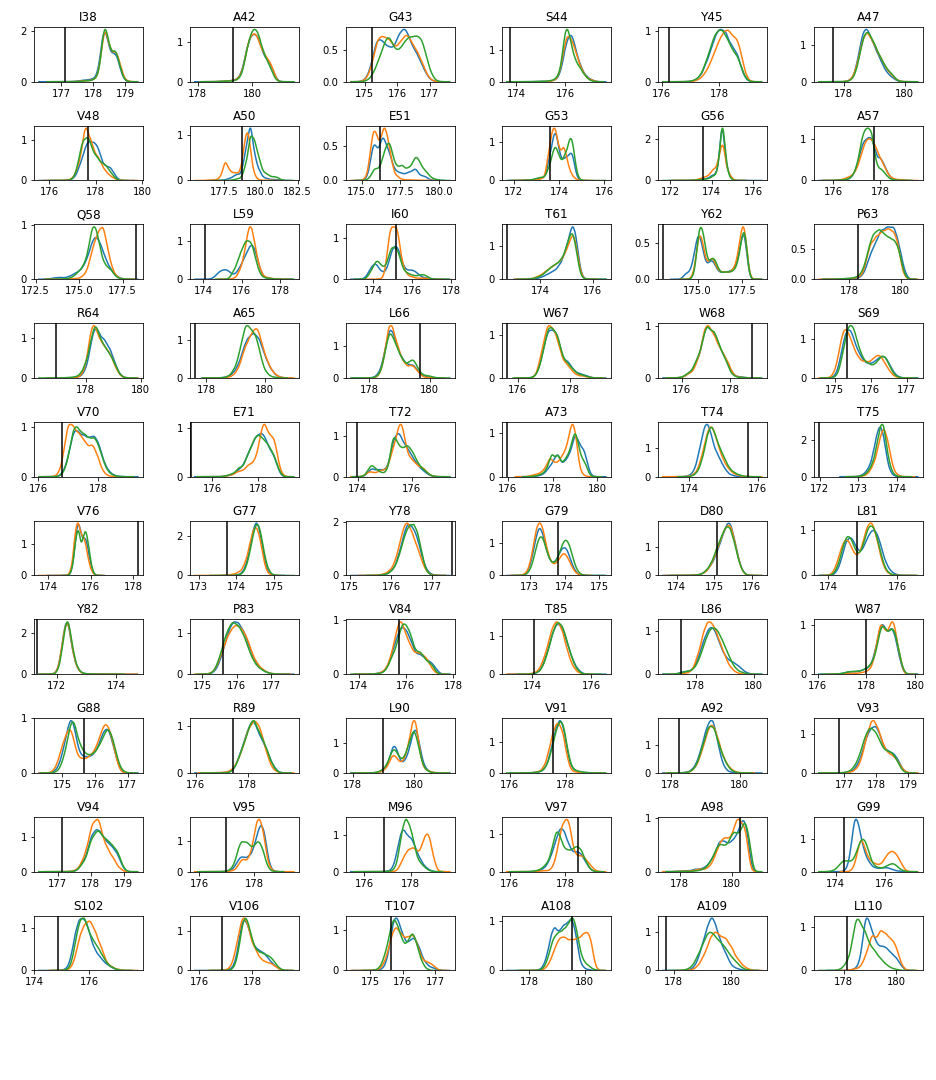
\includegraphics[width=\textwidth]{figures_SI/hist_shiftx2_C.png}
	 \caption{\scriptsize
 Probability distributions of the raw simulated CS of the MD trajectory snapshots for the different residues assigned spectroscopically for the C nucleus and the CS prediction method SHIFTX2. Three different states are compared: Partially Open (blue), Fully Open (orange) and Closed (green). The vertical line indicates the NMR determined experimental CS for the activated state. The distributions are calculated using kernel density estimation as implemented in the python library Seaborn. 
}
\label{SI_hist3}
\end{figure*}

\begin{figure*}[tbp]
	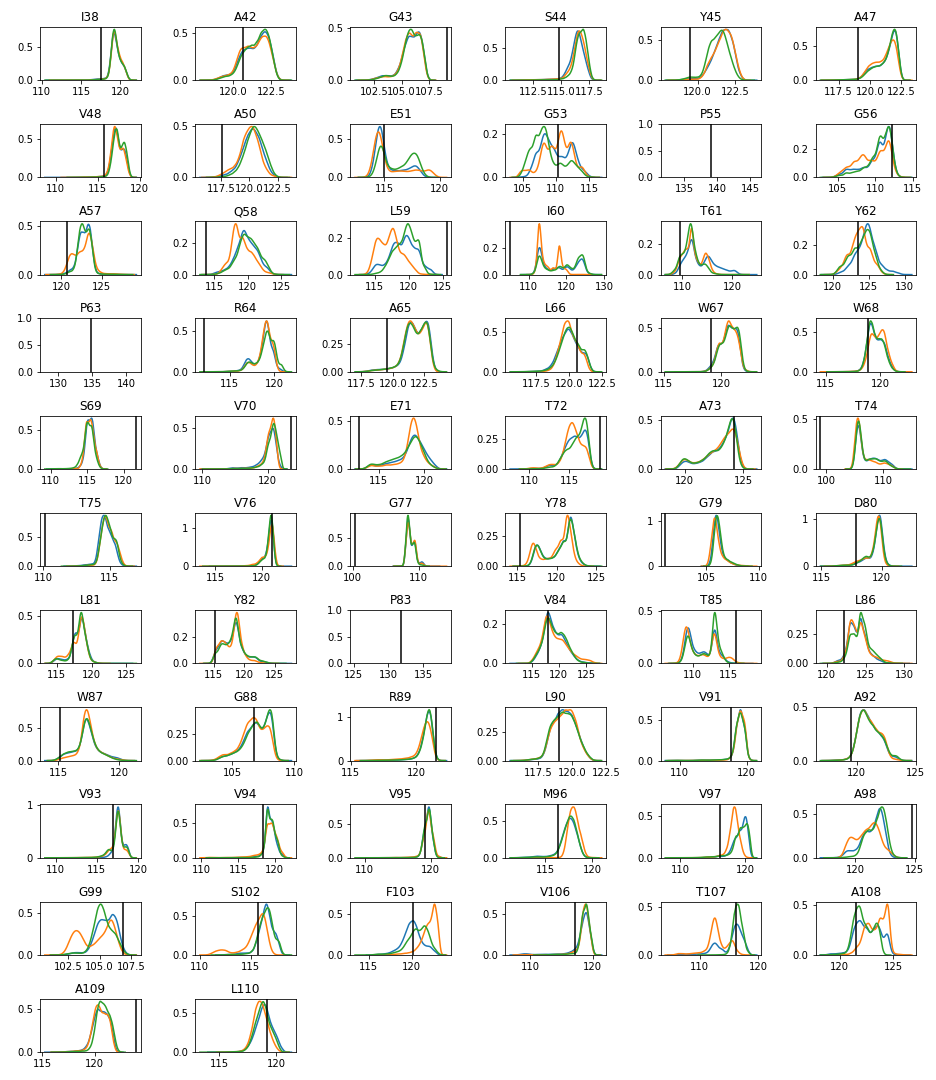
\includegraphics[width=\textwidth]{figures_SI/hist_shiftx2_N.png}
	 \caption{\scriptsize
 Probability distributions of the raw simulated CS of the MD trajectory snapshots for the different residues assigned spectroscopically for the N nucleus and the CS prediction method SHIFTX2. Three different states are compared: Partially Open (blue), Fully Open (orange) and Closed (green). The vertical line indicates the NMR determined experimental CS for the activated state. The distributions are calculated using kernel density estimation as implemented in the python library Seaborn. 
}
\label{SI_hist4}
\end{figure*}

\begin{figure*}[tbp]
	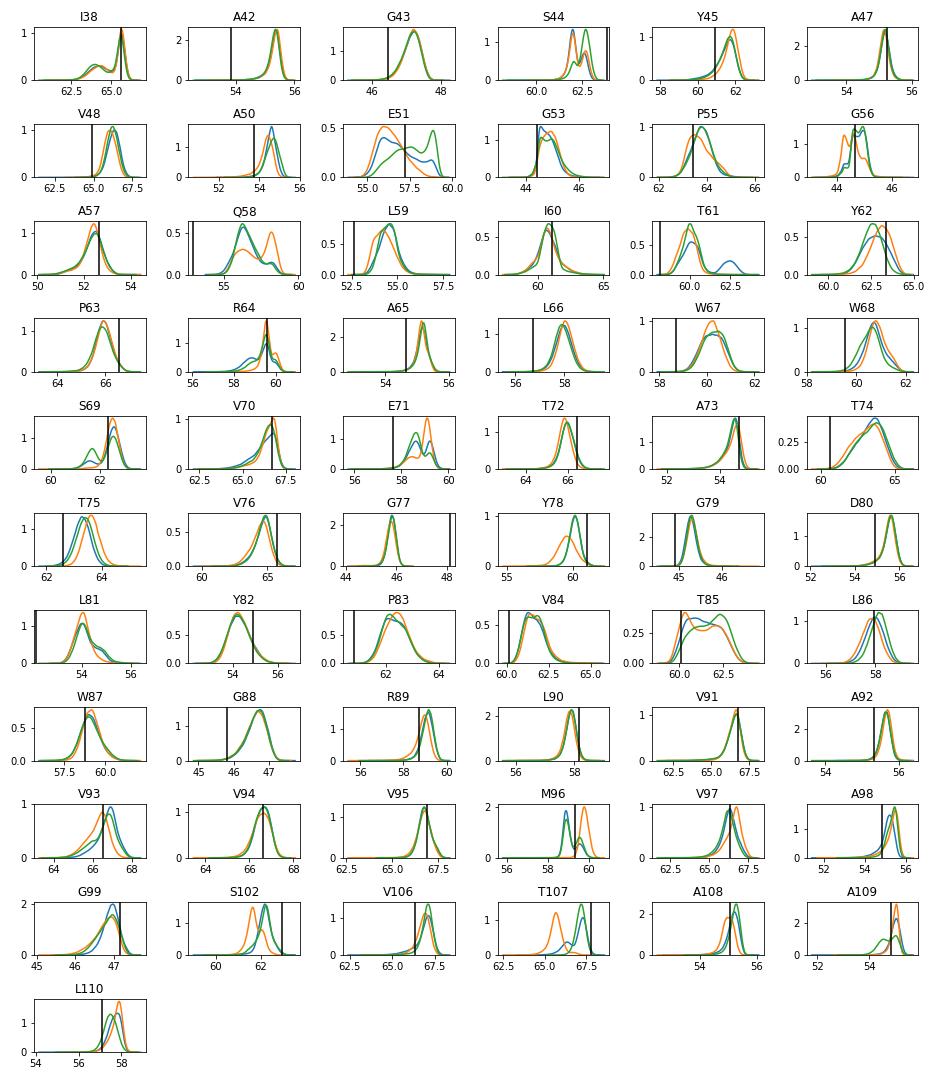
\includegraphics[width=\textwidth]{figures_SI/hist_sparta_plus_CA.png}
	 \caption{\scriptsize
 Probability distributions of the raw simulated CS of the MD trajectory snapshots for the different residues assigned spectroscopically for the \ca nucleus and the CS prediction method SHIFTX2. Three different states are compared: Partially Open (blue), Fully Open (orange) and Closed (green). The vertical line indicates the NMR determined experimental CS for the activated state. The distributions are calculated using kernel density estimation as implemented in the python library Seaborn. 
}
\label{SI_hist5}
\end{figure*}

\begin{figure*}[tbp]
	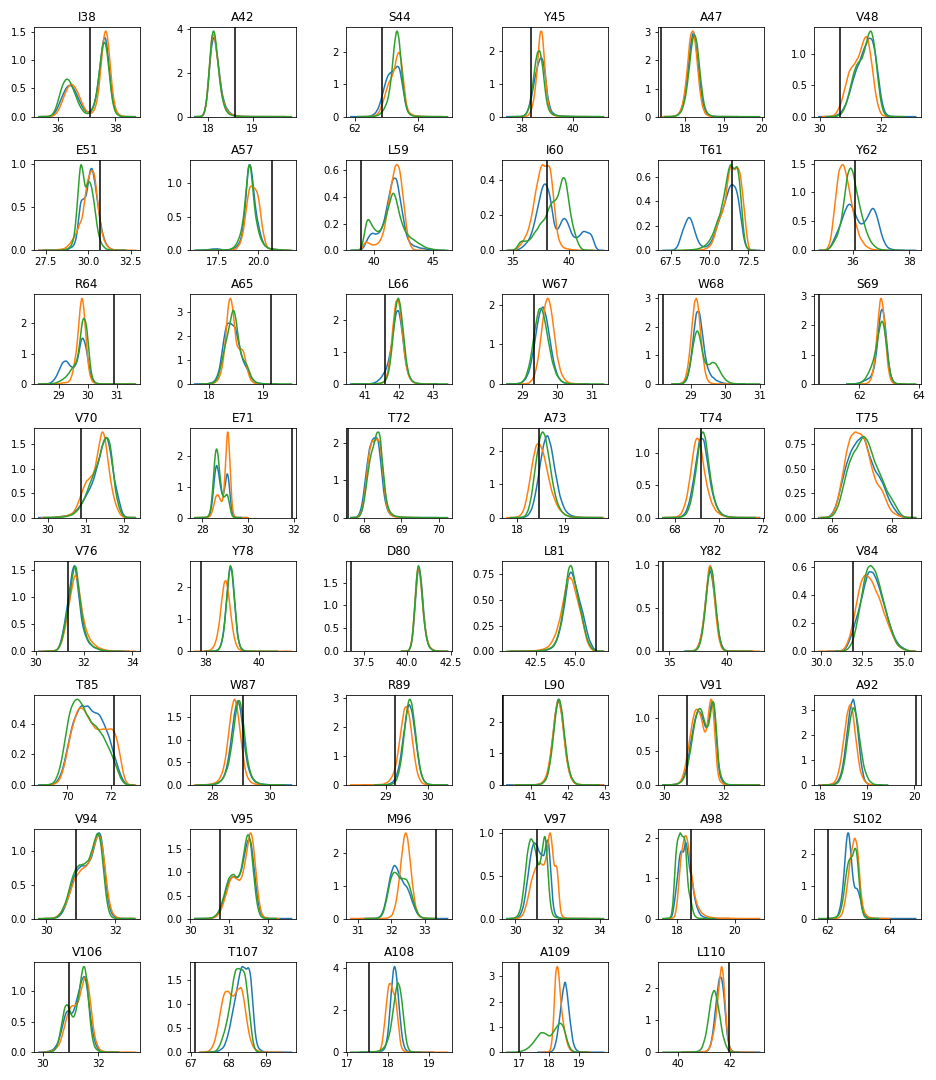
\includegraphics[width=\textwidth]{figures_SI/hist_sparta_plus_CB.png}
	 \caption{\scriptsize
 Probability distributions of the raw simulated CS of the MD trajectory snapshots for the different residues assigned spectroscopically for the \cb nucleus and the CS prediction method SHIFTX2. Three different states are compared: Partially Open (blue), Fully Open (orange) and Closed (green). The vertical line indicates the NMR determined experimental CS for the activated state. The distributions are calculated using kernel density estimation as implemented in the python library Seaborn. 
}
\label{SI_hist6}
\end{figure*}

\begin{figure*}[tbp]
	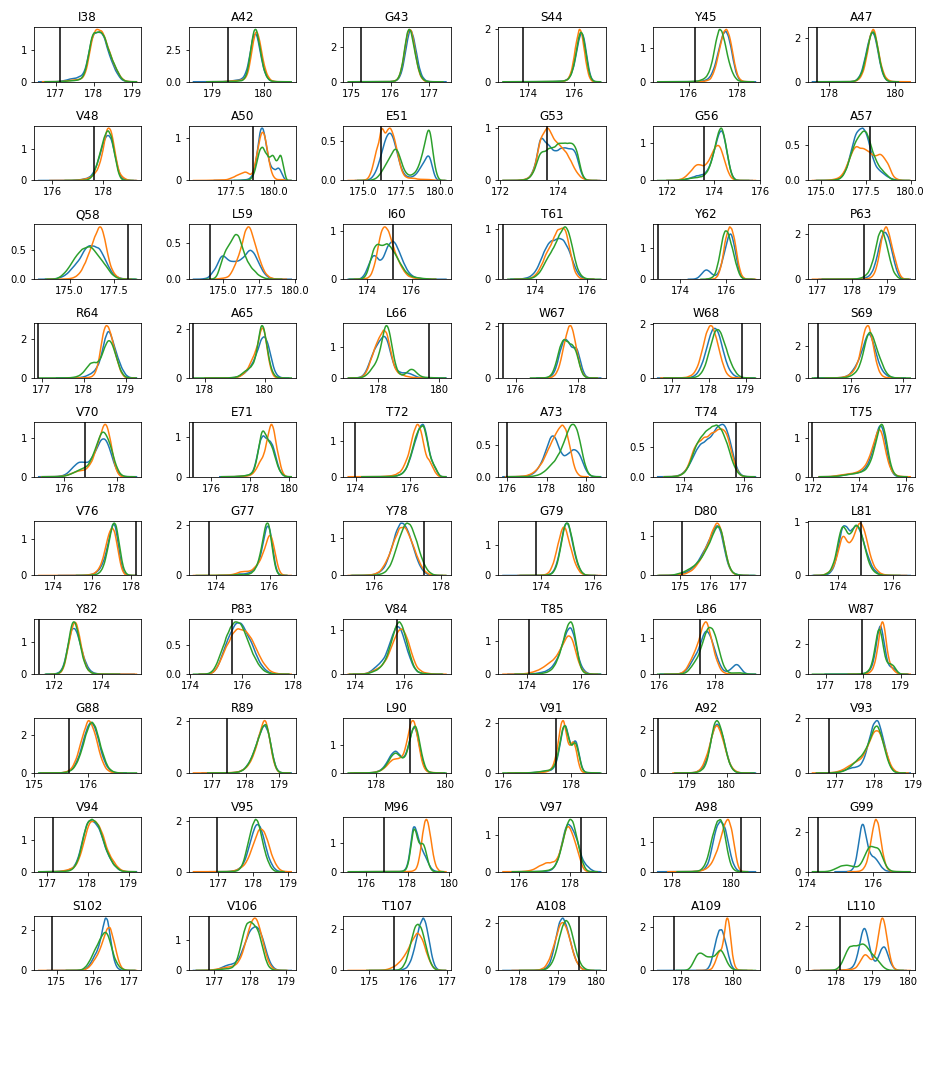
\includegraphics[width=\textwidth]{figures_SI/hist_sparta_plus_C.png}
	 \caption{\scriptsize
 Probability distributions of the raw simulated CS of the MD trajectory snapshots for the different residues assigned spectroscopically for the C nucleus and the CS prediction method SHIFTX2. Three different states are compared: Partially Open (blue), Fully Open (orange) and Closed (green). The vertical line indicates the NMR determined experimental CS for the activated state. The distributions are calculated using kernel density estimation as implemented in the python library Seaborn. 
}
\label{SI_hist7}
\end{figure*}

\begin{figure*}[tbp]
	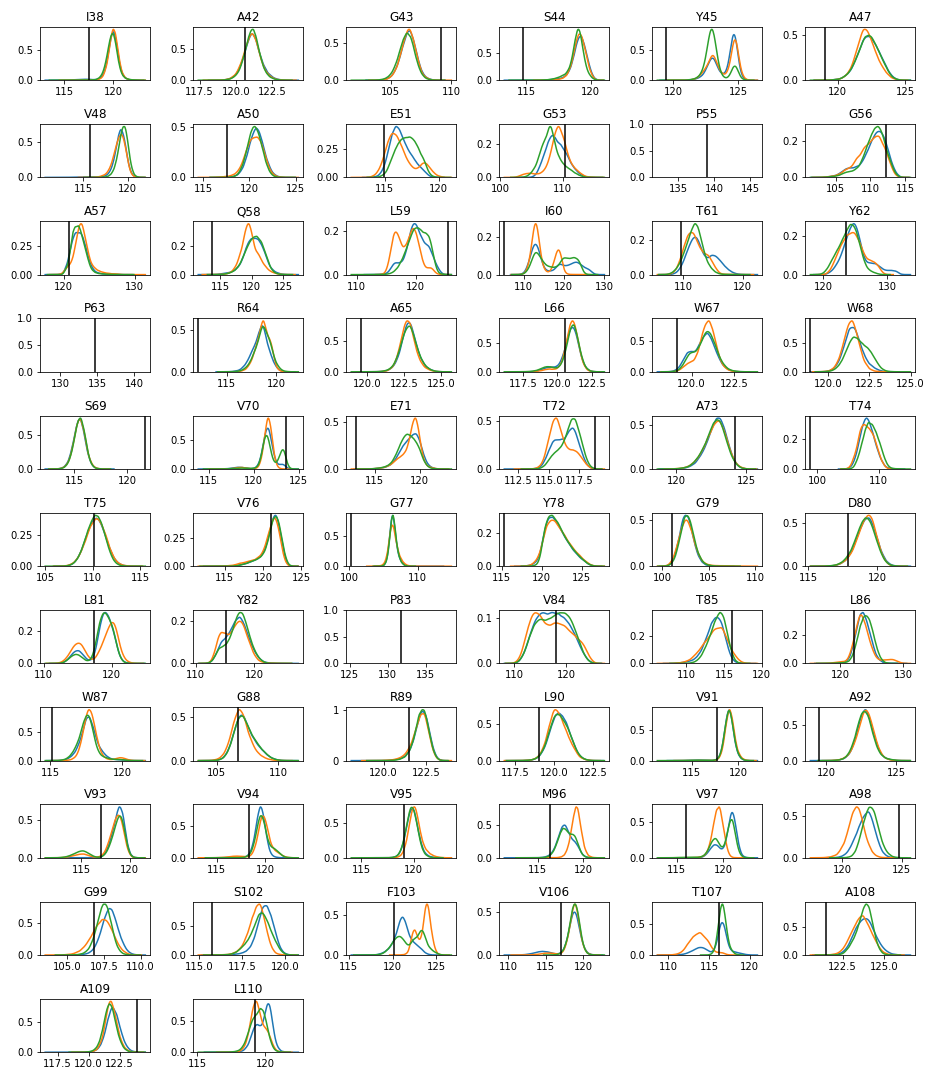
\includegraphics[width=\textwidth]{figures_SI/hist_sparta_plus_N.png}
	 \caption{\scriptsize
 Probability distributions of the raw simulated CS of the MD trajectory snapshots for the different residues assigned spectroscopically for the N nucleus and the CS prediction method SHIFTX2. Three different states are compared: Partially Open (blue), Fully Open (orange) and Closed (green). The vertical line indicates the NMR determined experimental CS for the activated state. The distributions are calculated using kernel density estimation as implemented in the python library Seaborn. 
}
\label{SI_hist8}
\end{figure*}

\begin{figure*}[tbp]
	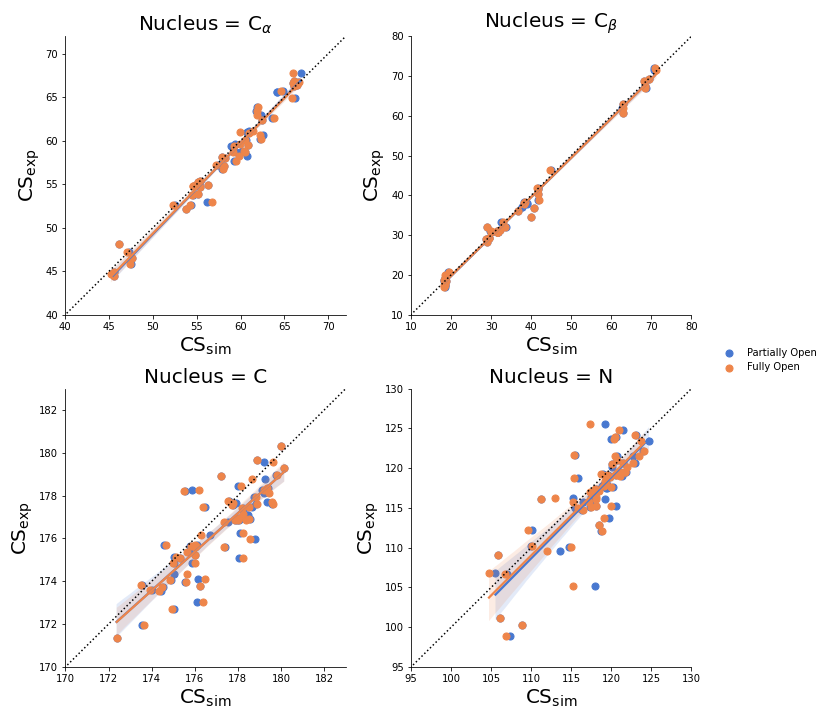
\includegraphics[width=\textwidth]{figures_SI/correlation_shiftx2_print.png}
	 \caption{\scriptsize
 Correlation diagram between experimental and simulated chemical shifts (shown in Figures \ref{SI_hist1}-\ref{SI_hist4}) for the Partially Open (blue) and Fully Open (orange) states for the nuclei studied and for the chemical shift prediction method SHIFTX2. 
}
\label{SI_corr1}
\end{figure*}

\begin{figure*}[tbp]
	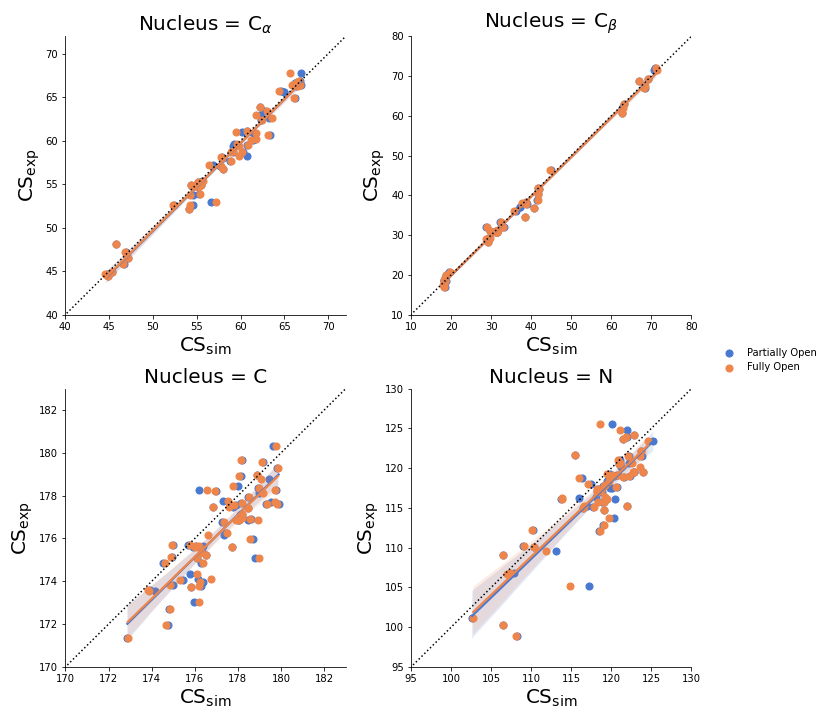
\includegraphics[width=\textwidth]{figures_SI/correlation_sparta_plus_print.png}
	 \caption{\scriptsize
 Correlation diagram between experimental and simulated chemical shifts (shown in Figures \ref{SI_hist5}-\ref{SI_hist8}) for the Partially Open (blue) and Fully Open (orange) states for the nuclei studied and for the chemical shift prediction method SPARTA+. 
}
\label{SI_corr2}
\end{figure*}

%\begin{landscape}
\begin{sidewaysfigure}[tbp]
	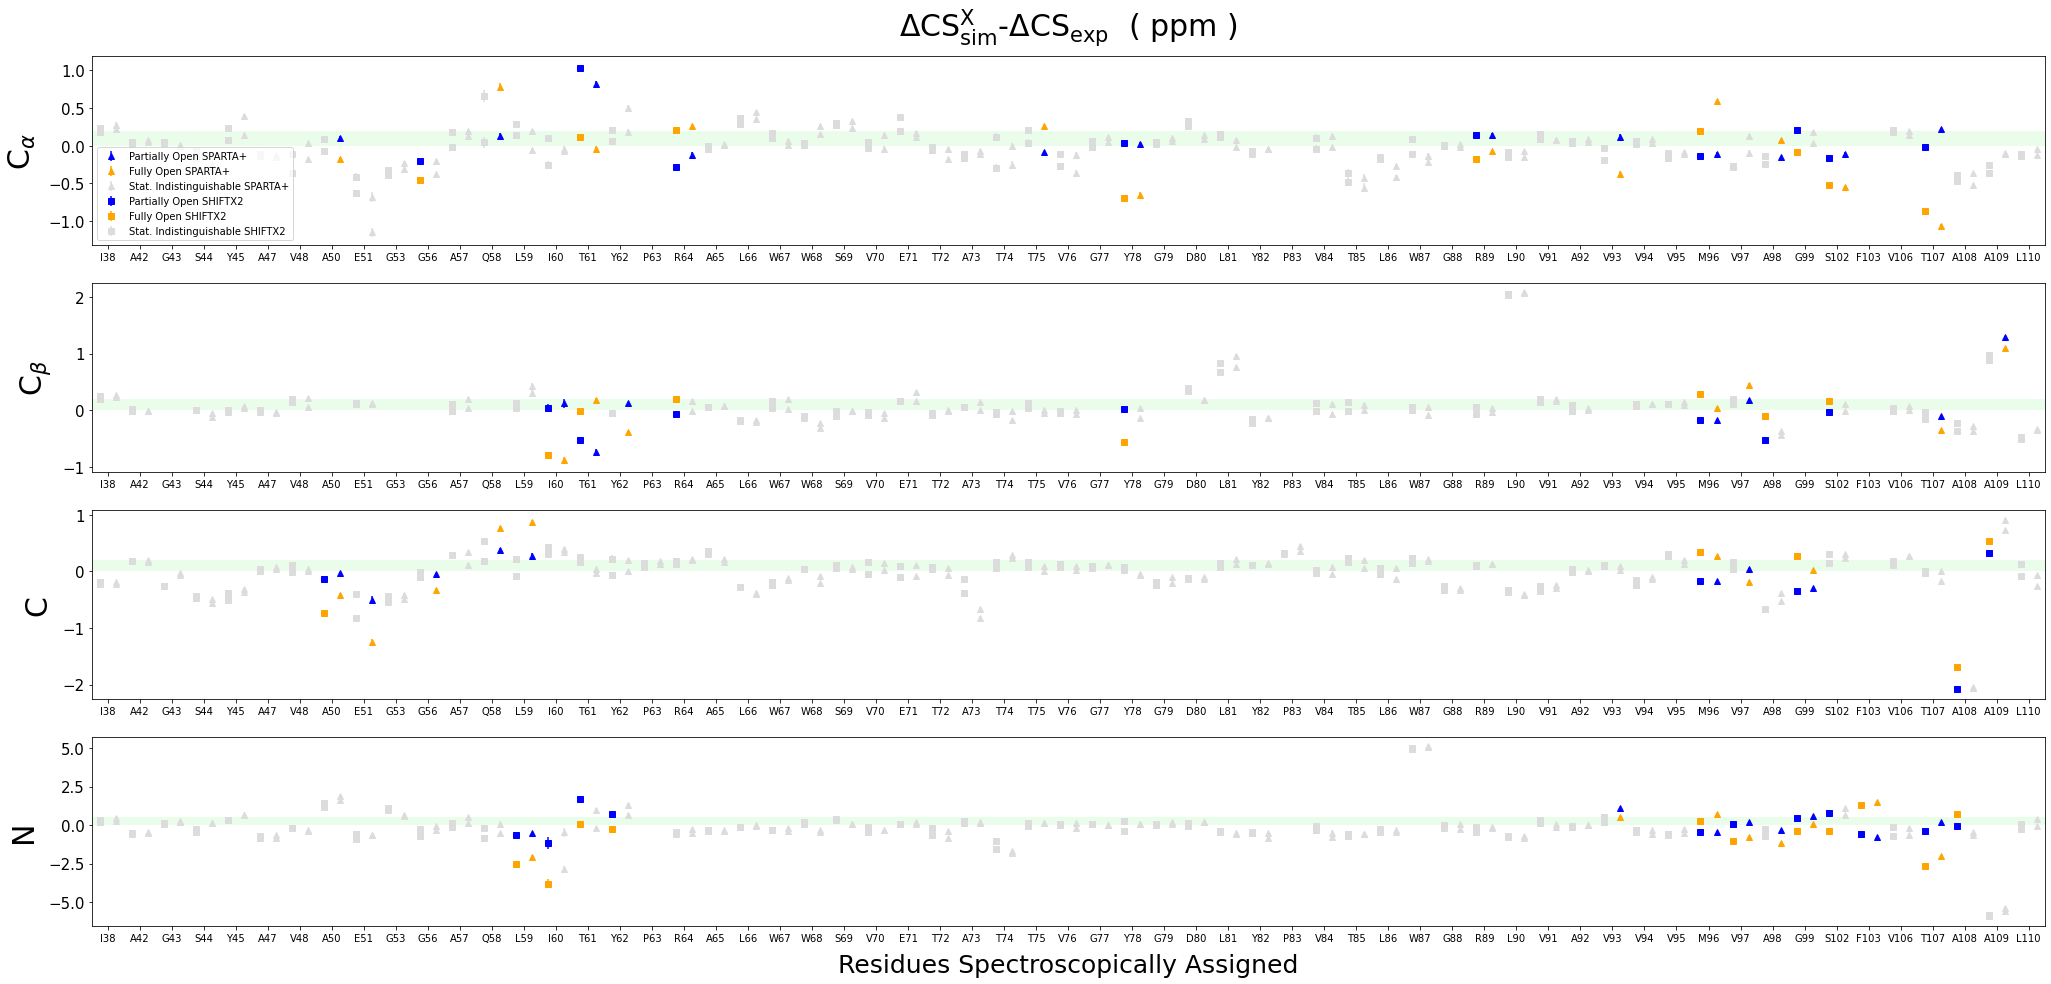
\includegraphics[width=\textwidth]{figures_SI/assignment_skew_model_all_print.png}
	 \caption{\scriptsize
Centers of 94$\%$ credible intervals of the difference in relative chemical shifts between experiment and simulation ($\Delta\text{CS}_{\text{sim}}^{\text{X}}-\Delta\text{CS}_{\text{exp}}$). The limits of the credible interval are shown as error bars. Both experiment and simulation use as reference the closed state chemical shifts: $\Delta\text{CS}_{\text{sim}}^{\text{X}}$ = CS$_{\text{sim}}^{\text{X}}$ - CS$_{\text{sim}}^{\text{C}}$  and $\Delta\text{CS}_{\text{exp}}$ = CS$_{\text{exp}}^{\text{pH}=4}$ - CS$_{\text{exp}}^{\text{pH}=7.5}$, where X represents the FO or PO sate. All residues on the x-axis for the different nuclei and chemical shift prediction methods. The agreement between MD simulations and the NMR experiments is higher the closer the value is to zero. Chemical shifts predicted by SPARTA+ and SHIFTX2 are drawn with triangles and squares respectively. The PO state (blue) has in general a better agreement with experiment than FO state (orange). The green shade depicts the typical experimental uncertainty. If two methods produce statistically identical CS or the signal is missing in the spectrum, the symbols are represented in gray.}
\label{SI_assignment_all}
\end{sidewaysfigure}
%\end{landscape}

\begin{figure*}[tbp]
	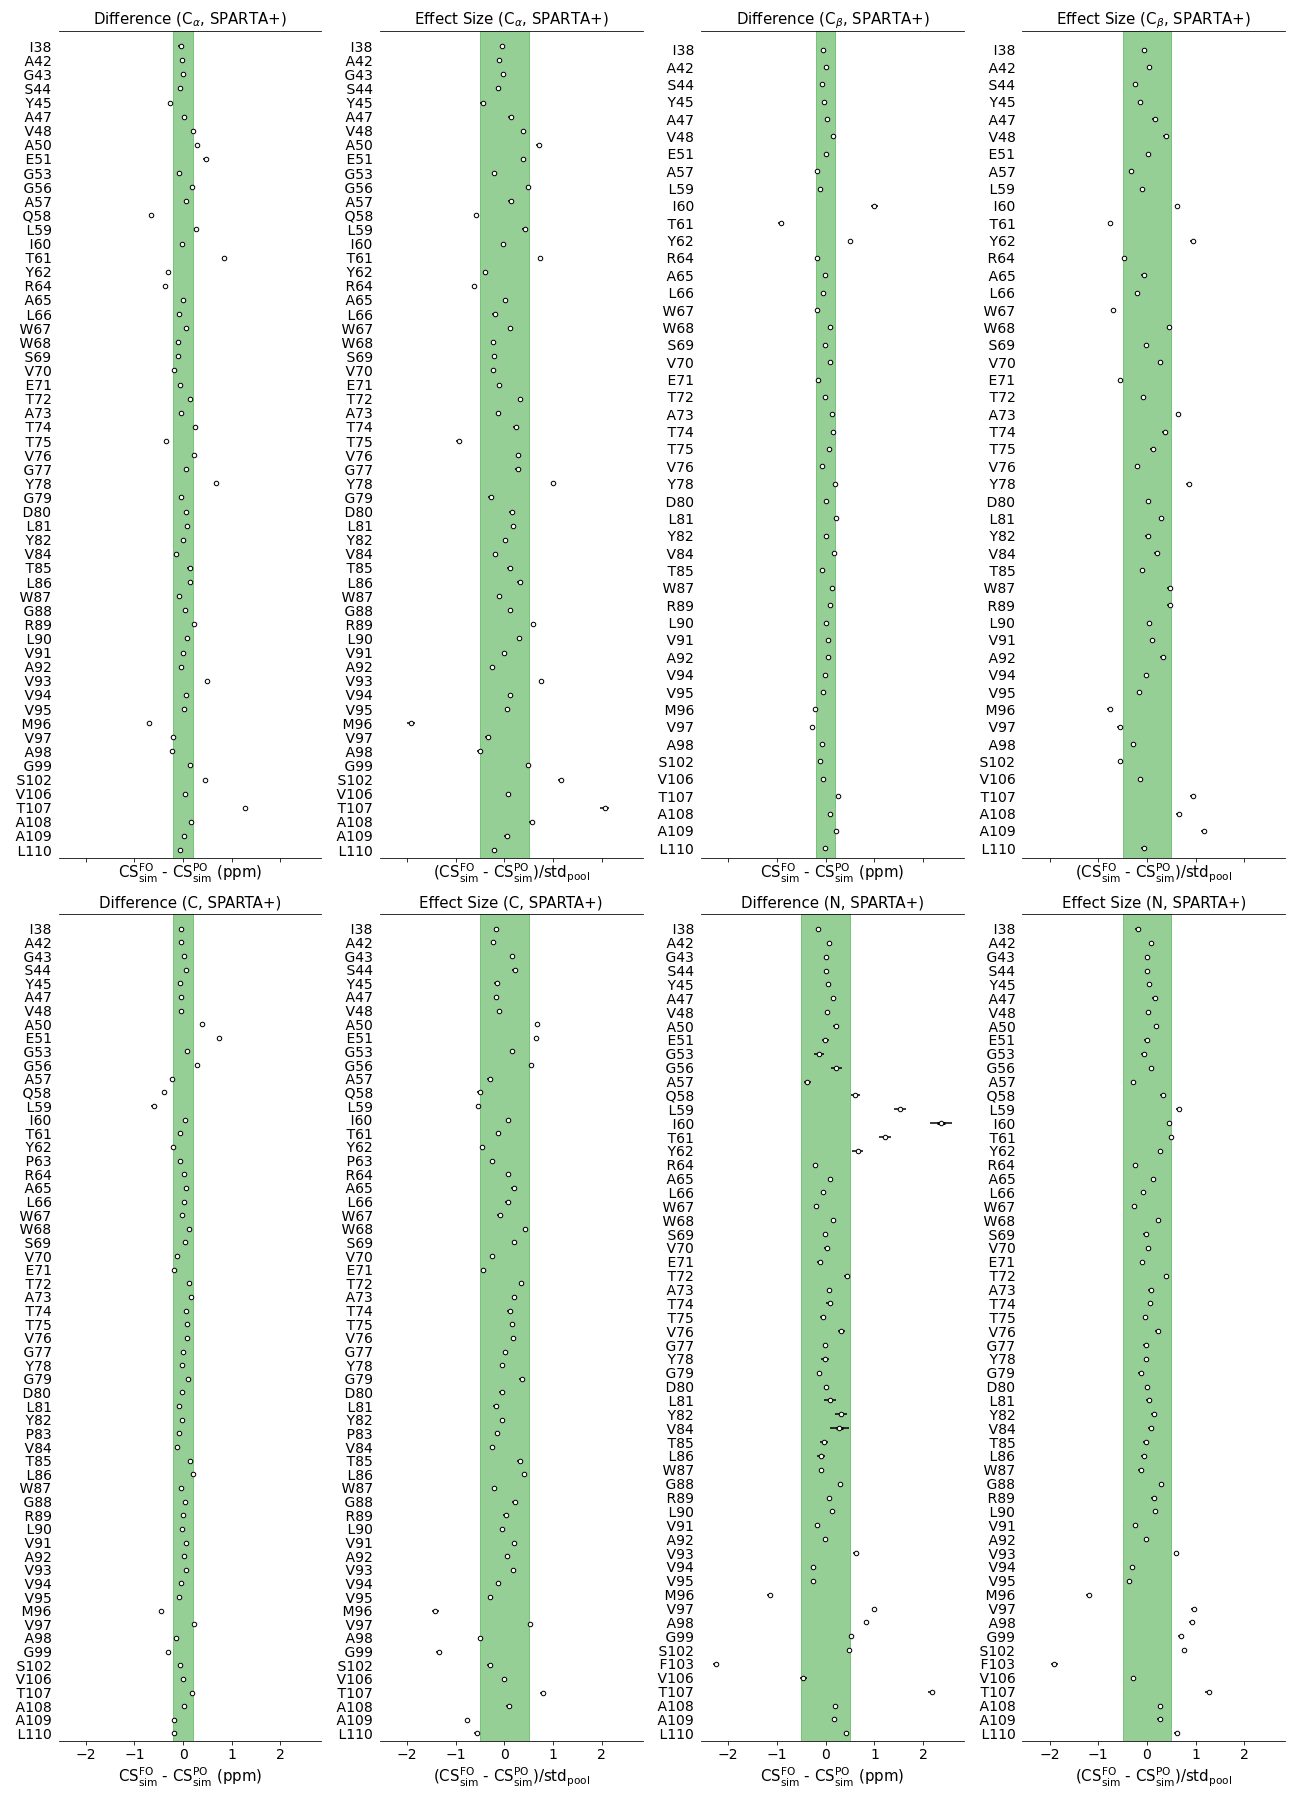
\includegraphics[width=0.85\textwidth]{figures_SI/statistical_filtering_skew_model_sparta_plus_all.png}
	 \caption{\scriptsize
 Statistical filtering of simulated signals to discover discriminating residues using the CS prediction method SPARTA+. Horizontal bars represent the 94\% credible interval of the variable distributions and circles represent its center. 
}
\label{SI_stat_filt_1}
\end{figure*}

\begin{figure*}[tbp]
	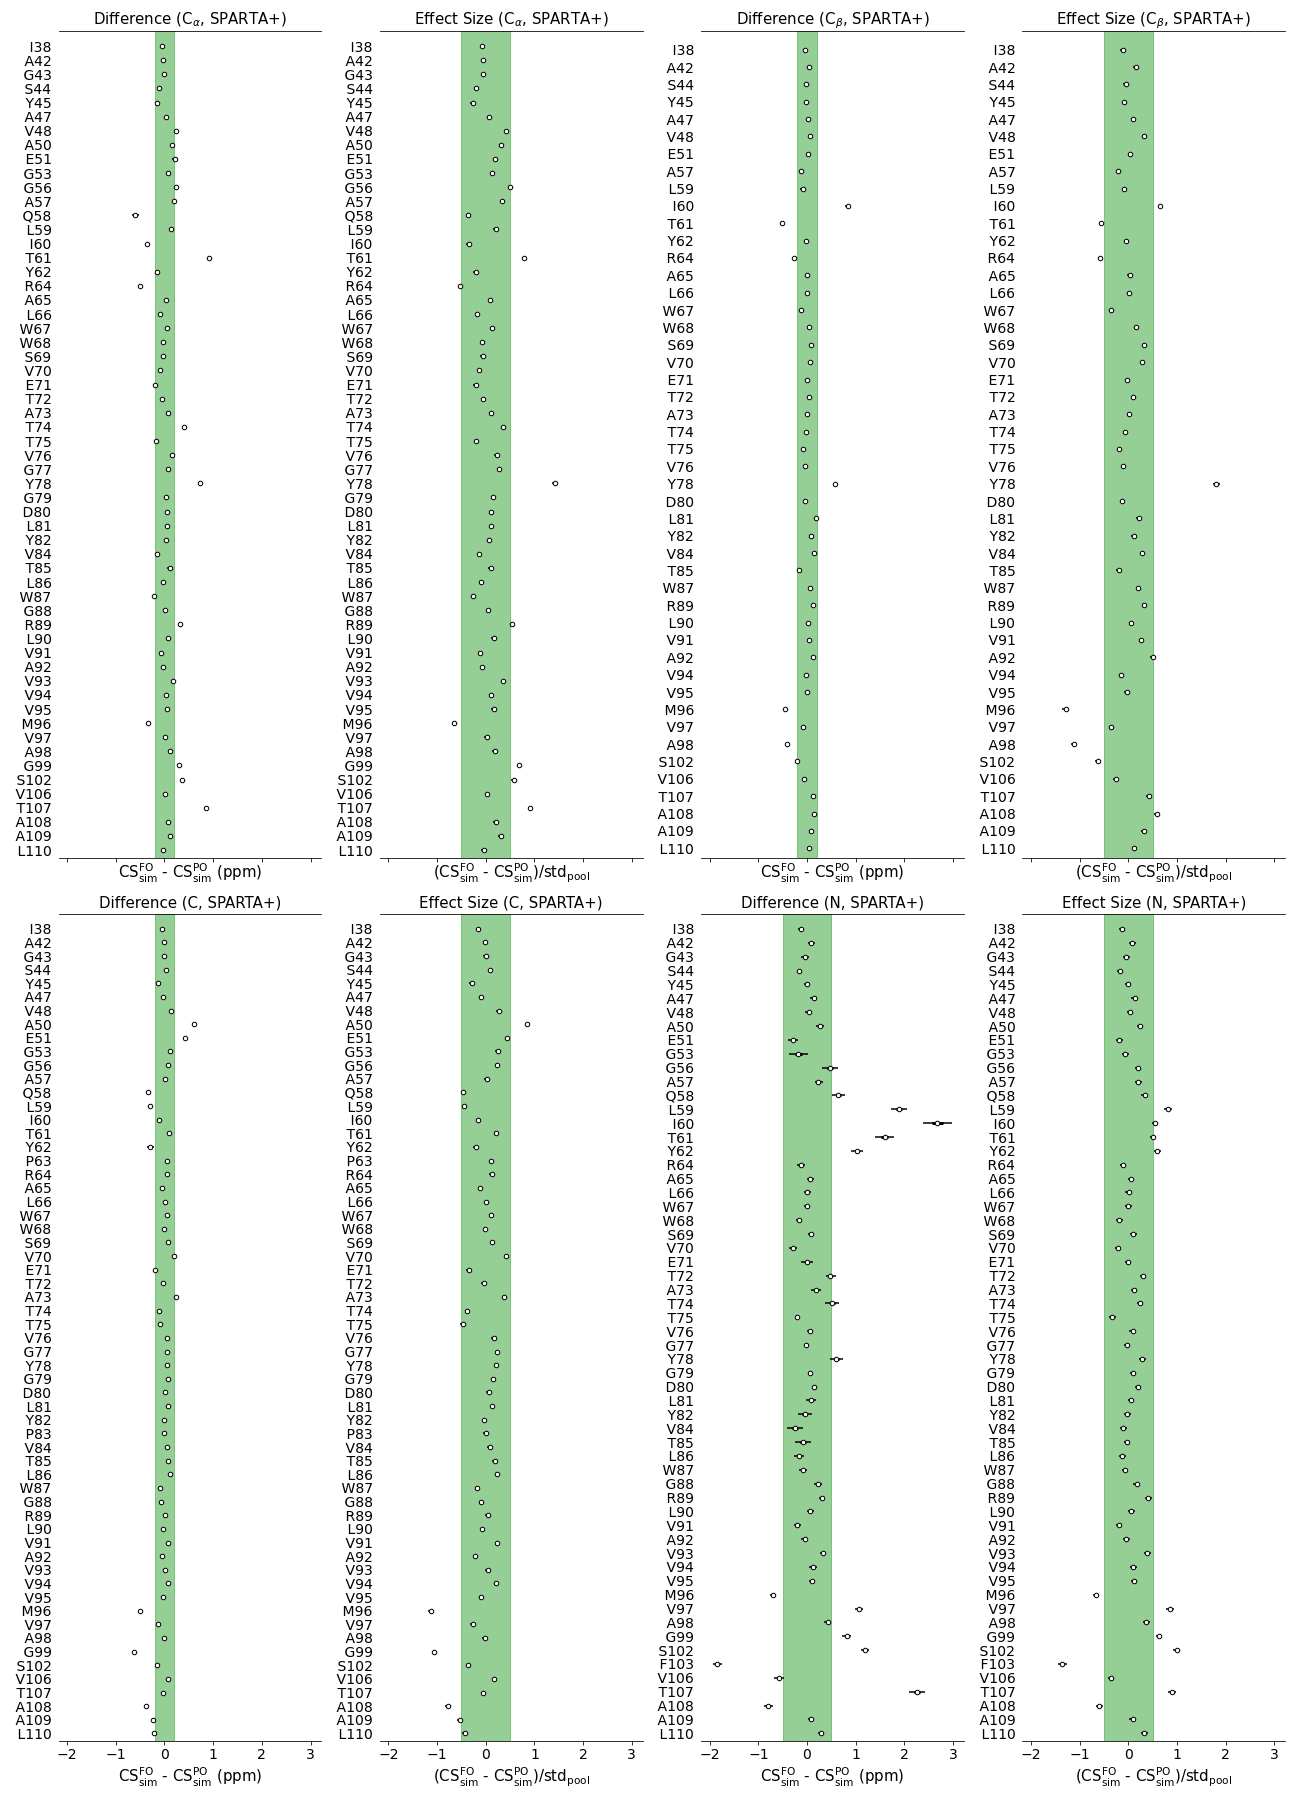
\includegraphics[width=0.85\textwidth]{figures_SI/statistical_filtering_skew_model_shiftx2_all.png}
	 \caption{\scriptsize
 Statistical filtering of simulated signals to discover discriminating residues using the CS prediction method SHIFTX2. Horizontal bars represent the 94\% credible interval of the variable distributions and circles represent its center.
}
\label{SI_stat_filt_2}
\end{figure*}

\begin{figure*}[tbp]
	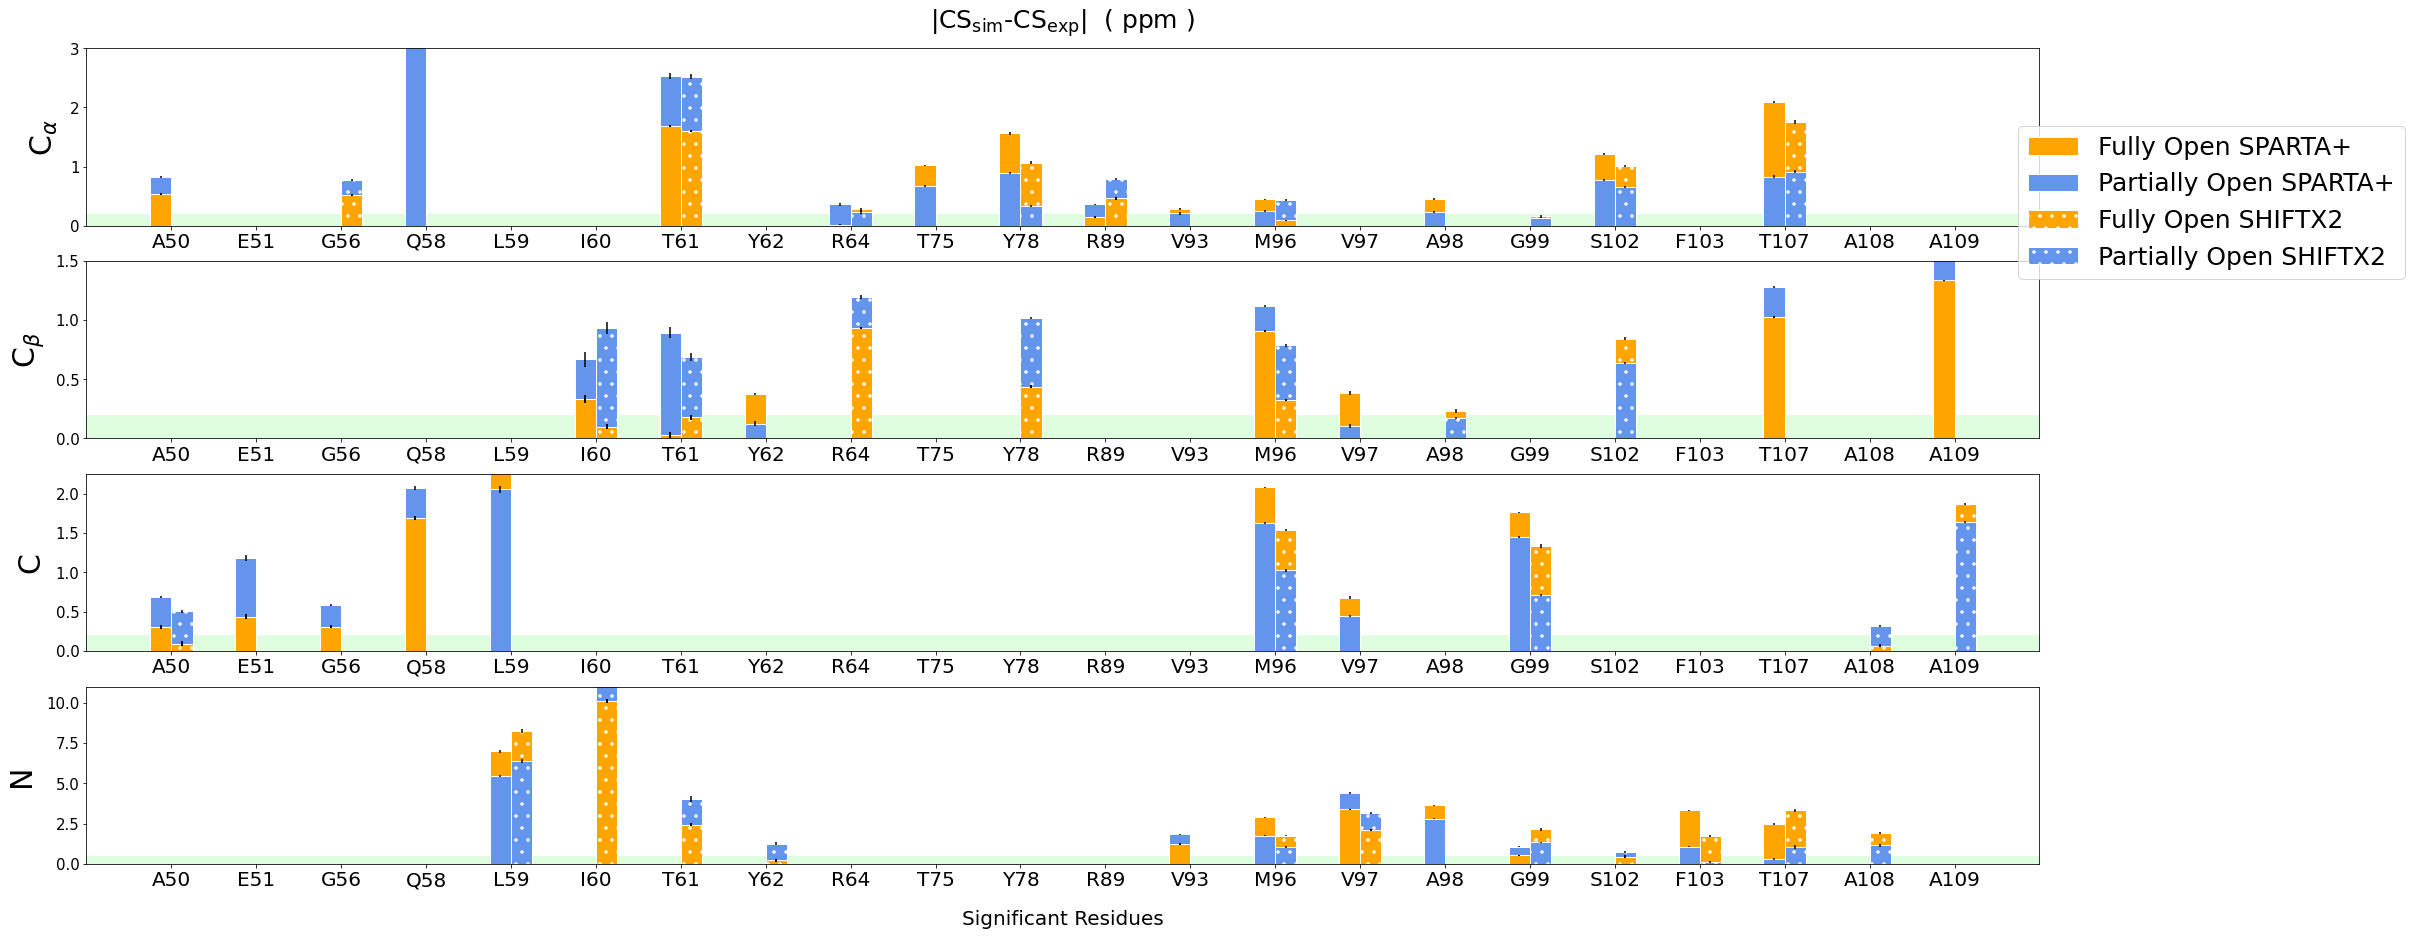
\includegraphics[width=\textwidth]{figures_SI/assignment_skew_model_markers_no_refernce_print.png}
	 \caption{\scriptsize
Centers of 94\% credible intervals for the difference in chemical shifts between experiment and simulation in absolute value ($|\text{CS}_{\text{sim}}^{\text{X}}-\text{CS}_{\text{exp}}|$). The limits of the credible interval are shown as error bars. The residues found to be discriminating residues using our statistical criteria are represented on the x-axis for the different nuclei and chemical shift prediction methods. The agreement to experiment is higher the closer the value is to zero. The green shade depicts the typical experimental uncertainty. The absence of a reference state increases the noise in the data. 
}
\label{SI_assignment_no_ref}
\end{figure*}

\begin{figure*}[tbp]
	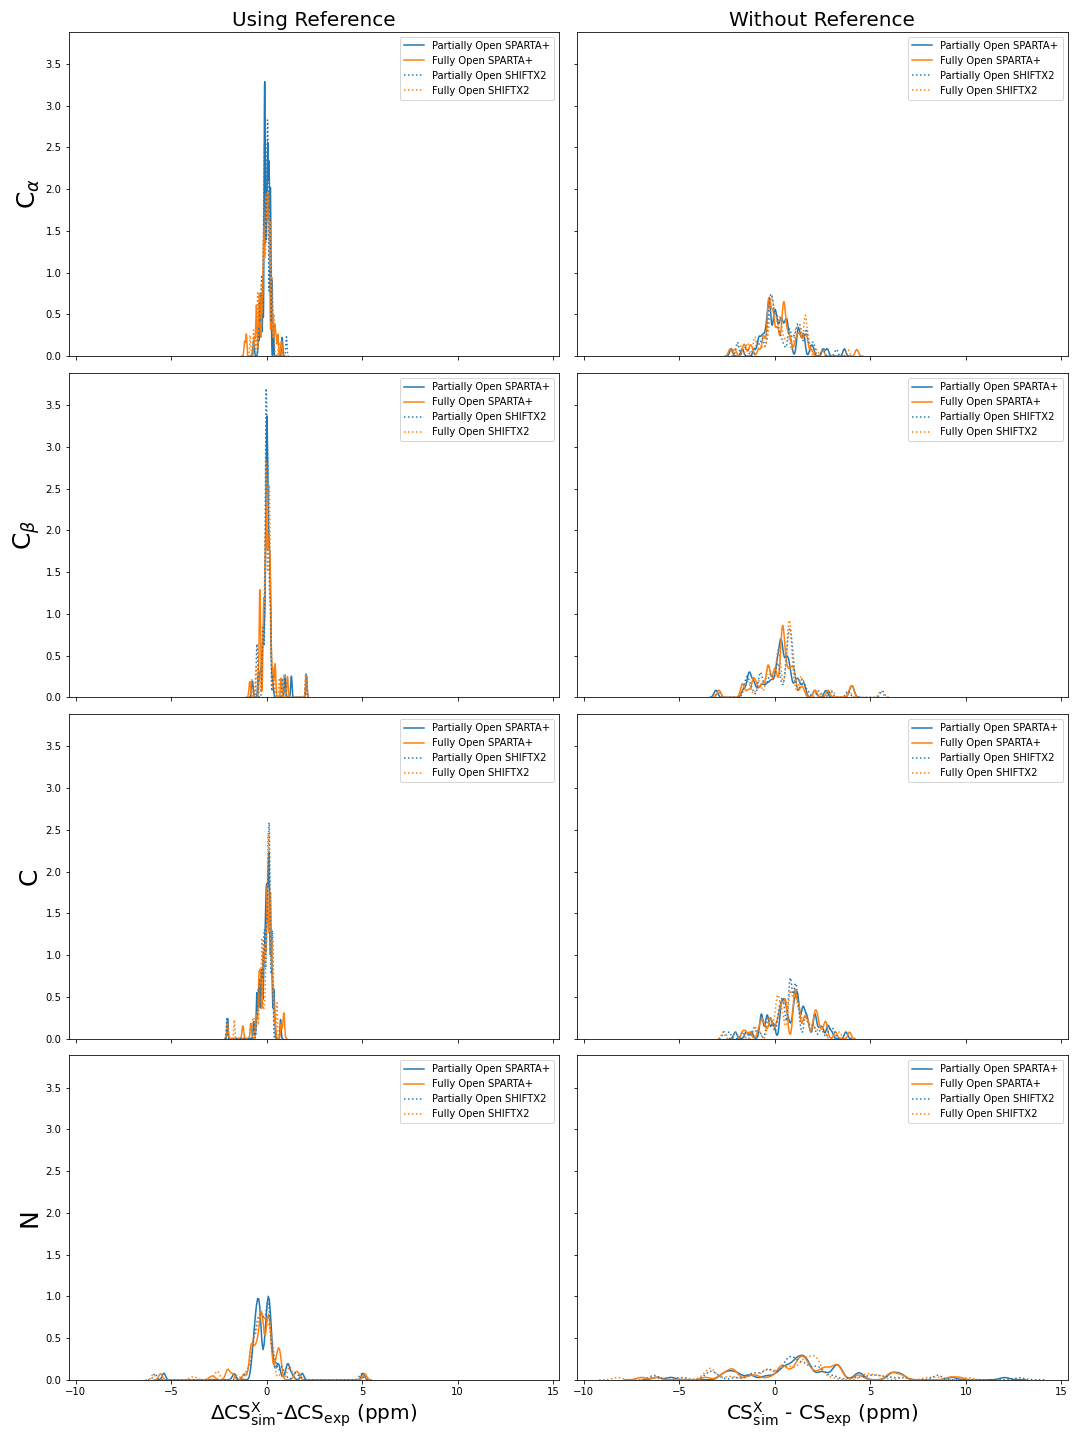
\includegraphics[width=0.85\textwidth]{figures_SI/error_distribution_print.png}
	 \caption{\scriptsize
Distributions of the CS simulation-experiment difference for the different nuclei (rows), for the two CS prediction methods (SPARTA+ solid line and SHIFTX2 dotted line) and for the two conductive states (Partially Open, blue and Fully Open, orange). These differences with experiment can be done using the CS of the closed state as a reference ($\Delta\text{CS}_{\text{sim}}^{\text{X}}-\Delta\text{CS}_{\text{exp}}$, left column) or without a reference ($\text{CS}_{\text{sim}}^{\text{X}}-\text{CS}_{\text{exp}}$ right column). The distributions without using the closed reference state are sharper and therefore using a reference state cancels random and systematic errors. The distributions are calculated using kernel density estimation as implemented in the python library Seaborn. 
}
\label{SI_error_dist}
\end{figure*}

\begin{figure}[tbp]
	\includegraphics[width=0.85\textwidth]{figures_SI/SPARTA_histograms-01.eps}
	 \caption{\scriptsize
Distributions of the CS simulation-experiment difference, $\text{CS}_{\text{sim}}^{\text{X}}-\text{CS}_{\text{exp}}$, for SPARTA+ and for the two conductive states (Partially Open, blue and Fully Open, orange). Each distribution is fit to a normal distribution function, shown inset with fitted values for PO (blue), and FO (orange).
}
\label{SI_sparta_histogram}
\end{figure}
\clearpage

\begin{figure}[tbp]
	\includegraphics[width=0.85\textwidth]{figures_SI/SHIFTX2_histograms-02.eps}
	 \caption{\scriptsize
Distributions of the CS simulation-experiment difference, $\text{CS}_{\text{sim}}^{\text{X}}-\text{CS}_{\text{exp}}$, for SHIFTX2 and for the two conductive states (Partially Open, blue and Fully Open, orange). Each distribution is fit to a normal distribution function, shown inset with fitted values for PO (blue), and FO (orange).
}
\label{SI_shiftx2_histogram}
\end{figure}
\clearpage

\begin{figure*}[tbp]
	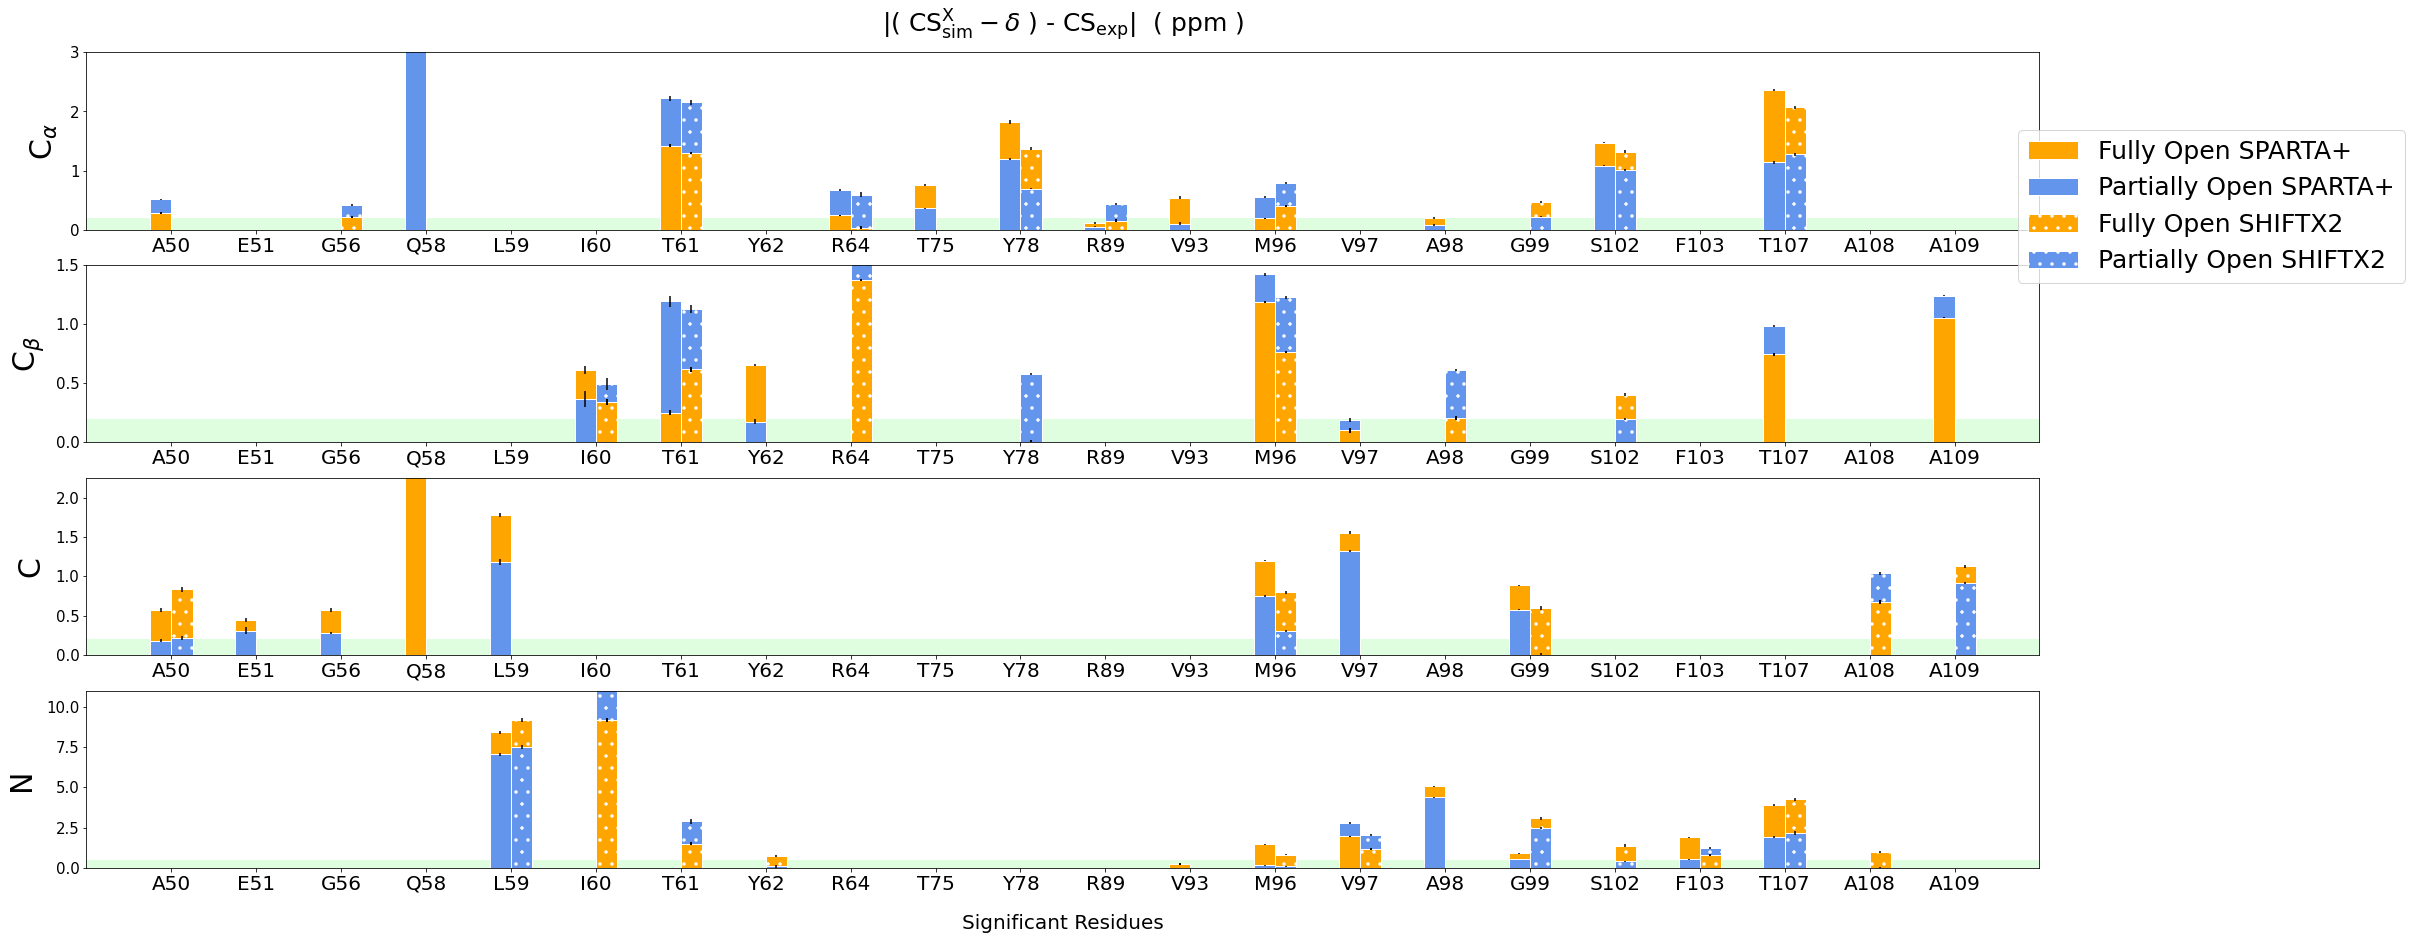
\includegraphics[width=\textwidth]{figures_SI/assignment_skew_model_markers_shifted_print.png}
	 \caption{\scriptsize
Centers 94\% credible intervals of the difference in chemical shifts between experiment and simulation in absolute value ($|(\text{CS}_{\text{sim}}^{\text{X}}-\delta)-\text{CS}_{\text{exp}}|$) where the simulated chemical shift has been corrected by $\delta$. $\delta$ is the position of the a fitted gaussian distribution to the chemical shifts of a nuclei-type (See Figures \ref{SI_shiftx2_histogram}-\ref{SI_sparta_histogram}). The limits of the credible interval are shown as error bars. The residues found to be discriminating residues using our statistical criteria are represented on the x-axis for the different nuclei and chemical shift prediction methods. The agreement to experiment is higher the closer the value is to zero. The green shade depicts the typical experimental uncertainty. The absence of a reference state increases the noise in the data. 
}
\label{SI_assignment_shift}
\end{figure*}

\clearpage

\begin{figure}[tbp]
\includegraphics[width=0.95\textwidth]{figures_SI/SI_Markers_FlowChart_v4-04.eps}
\caption{\label{SI_FlowChart} \scriptsize
    Flow chart demonstrating the combinations of the $\Delta\text{CS}_{\text{sim}}^{\text{X}}$ and $\Delta\text{CS}_{\text{exp}}$ that yield various classifications of the state markers identified in this study. A threshold of tolerance of 0.2 ppm for \ce{^13C} and 0.5 ppm for \ce{^15N}, based on the experimental tolerance, was used to determine if the CS change was significant. The resonances that are identified by Bayesian inference from the MD simulation data as distinguishing between FO and PO are shown, on the right, within the classification that they were determined to belong. Two different classifications for each state marker are possible due to the two chemical shift prediction tools. These are marked with what chemical shift prediction tool was used for each resonance and classification type (SH = SHIFTX2 and S+ = SPARTA+). The state that determined to be likely based on the calculation of $\Delta\Delta\text{CS}^{\text{X}}$ is shown as an orange (FO) and blue (PO) box. Dashed boxes are used to indicate when one CS prediction tool was inconclusive and the other determined a state. Resonances that were determined to be inconclusive are shown without a thin box around them. FO = fully open, PO = partially open, C = closed, $\Delta\text{CS}_{\text{sim}}^{\text{X}}$ = $\text{CS}_{\text{sim}}^{\text{X}}$ - $\text{CS}_{\text{sim}}^{\text{Closed}}$, and $\Delta\text{CS}_{\text{exp}}$ = $\text{CS}_{\text{exp}}^{\text{pH}=4\text{, act}}$ - $\text{CS}_{\text{exp}}^{\text{pH}=7.5\text{, deact}}$.}
\end{figure}
\clearpage

\begin{figure*}[tbp]
	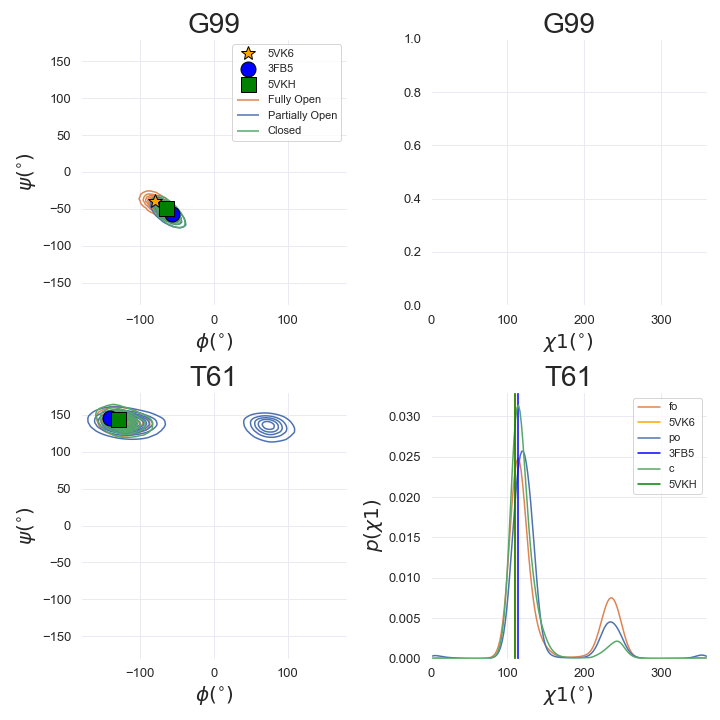
\includegraphics[width=0.85\textwidth]{figures_SI/dihedral_analysis_SI.png}
	 \caption{\scriptsize
Ramachandran and Janin diagrams (left and right columns, respectively) of the discriminating amino acids (rows) that are consistent with the Fully Open state as opposed to the Partially Open state consistent with most markers. The distributions are obtained from the dihedral angles obtained from the simulations of the Fully Open, Partially Open and Closed states. Additionally the values of the XRD structures are included as points or vertical lines.. Kernel density estimation is used to calculate the distributions as implemented in the Seaborn python library. 
}
\label{SI_dihedral}
\end{figure*}

\clearpage

\begin{figure*}[tbp]
	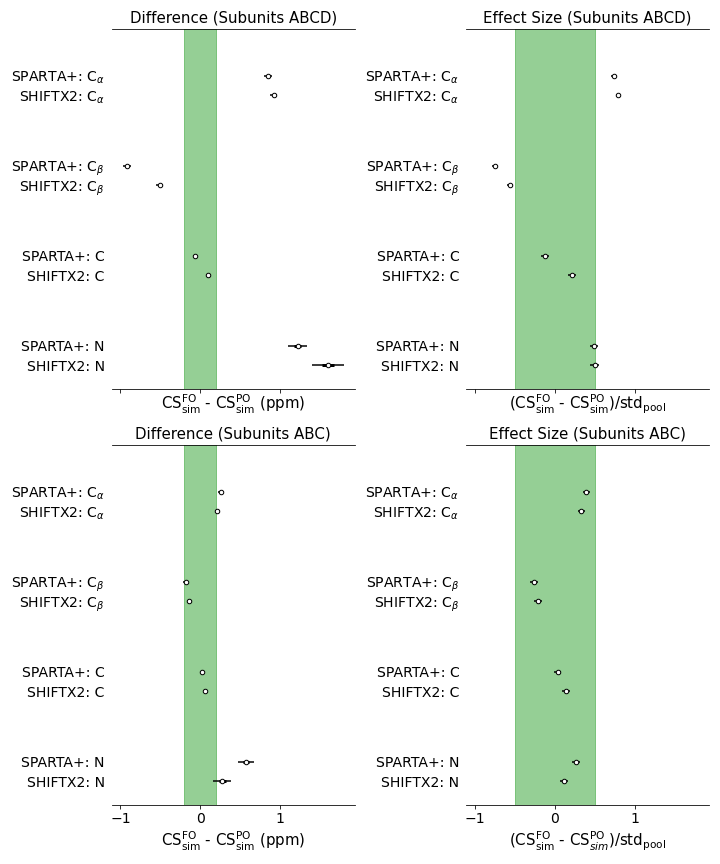
\includegraphics[width=0.85\textwidth]{figures_SI/statistical_filtering_skew_model_shiftx2_T61.png}
	 \caption{\scriptsize
Statistical filtering variables: difference in means and effect size for residue T61. The top graphs show the data using the four subunits of KcsA and the bottom graphs only subunits ABC. This figure shows that the reason why T61 is a discriminating residue is because one of the subunits has fluctuated away from the average. Horizontal bars represent the 94\% credible interval of the variable distributions and circles represent its center. 
}
\label{SI_stat_filt_T61}
\end{figure*}


\clearpage
\section{Supplementary Tables}

\begingroup
\begin{center}
\begin{longtable} {l|l|c|c|c}
\caption{\scriptsize Experimental parameters for the 3D experiments at 900 MHz. Pulse sequences similar to those used for these experiments are available at \url{comdnmr.nysbc.org}\label{SI_tb_900exp}}\\ \hline \hline
Experiment & & 3D NCACX & 3D NCOCX & 3D CANCO \\ \hline
\multicolumn{2}{l|}{ MAS frequency } & 16.666 kHz & 16.666 kHz & 16.666 kHz \\ \hline
\multicolumn{2}{l|}{ First transfer } & H-N CP & H-N CP & H-C CP \\ \hline
& $\omega_{1,\text{H}} / 2\pi$ (kHz) & 62 & 62 & 69 \\ \hline
& $\omega_{1,\text{N/C}} / 2\pi$ (kHz) & N: 50 & N: 50 & C: 59 \\ \hline
& Pulse shape & \ce{^1H} tangential & \ce{^1H} tangential & Linear ramp \\ \hline
& Contact time (ms) & 0.8 & 0.8 & 0.8 \\ \hline
\multicolumn{2}{l|}{ Second transfer } & N-C CP & N-C CP & C-N CP \\ \hline
& $\omega_{1,\text{H}} / 2\pi$ (kHz) & 94 & 91 & 91 \\ \hline
& $\omega_{1,\text{N/C}} / 2\pi$ (kHz) & C: 28 & C: 41 & C: 29 \\
& & N: 42 & N: 25 & N: 42  \\ \hline
& Shape: nucleus and range & \ce{^13C} tangential & \ce{^13C} tangential & \ce{^13C} tangential \\ \hline
& Contact time (ms) & 5 & 5.2 & 5.5 \\ \hline
\multicolumn{2}{l|}{ Third transfer } & C-C mixing & C-C mixing & N-C CP \\ \hline
& $\omega_{1,\text{H}} / 2\pi$ (kHz) & $\sim$17 & $\sim$17 & 98 \\ \hline
& $\omega_{1,\text{N/C}} / 2\pi$ (kHz) & & & C: 43 \\
& & & & N: 25 \\ \hline
& Shape: nucleus and range & & & \ce{^13C} tangential \\ \hline
& Contact time (ms) & 50 & 50 & 4.5 \\ \hline
& $\omega_{1,\text{H}} / 2\pi$ & & & 91 \\ \hline 
Scans & & 16 & 32 & 64 \\ \hline
Points & \ce{^13C} (direct) & 2048 & 2048 & 2048 \\ \hline
& \ce{^13C} & 248 & 110 & 50 \\ \hline
& \ce{^15N} & 60 & 80 & 48 \\ \hline
Acquisition time & \ce{^13C} (direct) (ms) & 12.3 & 12.3 & 12.3 \\ \hline
& \ce{^13C} (ms) & 6.6 & 6.6 & 7.2 \\ \hline
& \ce{^15N} (ms) & 7 & 7.2 & 6 \\ \hline
Sweep width & \ce{^13C} (direct) (ppm) & 368 & 368 & 368 \\ \hline
& \ce{^13C} (ppm) & 74 & 37 & 37 \\ \hline
& \ce{^15N} (ppm) & 50 & 46 & 46 \\ \hline
Carrier Frequency & \ce{^13C} (direct) (ppm) & 100.8 & 100.8 & 175.8 \\ \hline
& \ce{^13C} (ppm) & 60.8 & 175.8 & 60.8 \\ \hline
& \ce{^15N} (ppm) & 118.1 & 118.1 & 118.1 \\ \hline
Total time & & 5 d 12 h & 8 d & 7 d 14 h \\ \hline
\end{longtable}
\end{center}
\endgroup

\begingroup
\begin{center}
\begin{longtable} {l|l|c|c|c}
\caption{\scriptsize Experimental parameters for the 3D experiments at 750 MHz. Pulse sequences similar to those used for these experiments are available at \url{comdnmr.nysbc.org}\label{SI_tb_750exp}}\\ \hline \hline
Experiment & & 3D NCACX & 3D NCOCX & 3D CANCO \\ \hline
\multicolumn{2}{l|}{ MAS frequency } & 16 kHz & 16 kHz & 33.333 kHz \\ \hline
\multicolumn{2}{l|}{ First transfer } & H-N CP & H-N CP & H-C CP \\ \hline
& $\omega_{1,\text{H}} / 2\pi$ (kHz) & 72 & 72 & 80 \\ \hline
& $\omega_{1,\text{N/C}} / 2\pi$ (kHz) & N: 58 & N: 58 & C: 56 \\ \hline
& Pulse shape & \ce{^1H} tangential & \ce{^1H} tangential & \ce{^1H} tangential \\ \hline
& Contact time (ms) & 1 & 1 & 1 \\ \hline
\multicolumn{2}{l|}{ Second transfer } & N-C CP & N-C CP & C-N CP \\ \hline
& $\omega_{1,\text{H}} / 2\pi$ (kHz) & 95 & 95 & 95 \\ \hline
& $\omega_{1,\text{N/C}} / 2\pi$ (kHz) & C: 24 & C: 8 & C: 17 \\
& & N: 40 & N: 24 & N: 48 \\ \hline
& Shape: nucleus and range & \ce{^13C} tangential & \ce{^13C} tangential & \ce{^13C} tangential \\ \hline
& Contact time (ms) & 3.75 & 5.0 & 3.75 \\ \hline
\multicolumn{2}{l|}{ Third transfer } & C-C mixing & C-C mixing & N-C CP \\ \hline
& $\omega_{1,\text{H}} / 2\pi$ (kHz) & $\sim$16 & $\sim$16 & 95 \\ \hline
& $\omega_{1,\text{N/C}} / 2\pi$ (kHz) & & & C: 17 \\
& & & & N: 49 \\ \hline
& Shape: nucleus and range & & & \ce{^13C} tangential \\ \hline
& Contact time (ms) & 50 & 50 & 5.0 \\ \hline
& $\omega_{1,\text{H}} / 2\pi$ & & & 95 \\ \hline 
Scans & & 96 & 144 & 64 \\ \hline
Points & \ce{^13C} (direct) & 2000 & 2000 & 2100 \\ \hline
& \ce{^13C} & 90 & 60 & 130 \\ \hline
& \ce{^15N} & 32 & 32 & 36 \\ \hline
Acquisition time & \ce{^13C} (direct) (ms) & 12.8 & 12.8 & 13.44 \\ \hline
& \ce{^13C} (ms) & 5.625 & 5.625 & 7.02 \\ \hline
& \ce{^15N} (ms) & 6 & 6 & 7.8 \\ \hline
Sweep width & \ce{^13C} (direct) (ppm) & 414 & 414 & 414 \\ \hline
& \ce{^13C} (ppm) & 42.4 & 28.3 & 44.2 \\ \hline
& \ce{^15N} (ppm) & 35 & 35 & 33.7 \\ \hline
Carrier Frequency & \ce{^13C} (direct) (ppm) & 109.9 & 109.9 & 109.9 \\ \hline
& \ce{^13C} (ppm) & 58 & 176.5 & 58 \\ \hline
& \ce{^15N} (ppm) & 111.2 & 111.2 & 111.2 \\ \hline
Total time & & 5 d 1 h & 5 d 21 h & 5 d 7 h \\ \hline
\end{longtable}
\end{center}
\endgroup
\clearpage
\begingroup
\begin{center}
\begin{longtable} {|l|l|c|c|c|c|}
\caption{\scriptsize Root mean square errors (RMSE) of the different CS calculations of this work in relation to their experimental counter parts. FO stands for the Fully Open state (5VK6) and PO for the Partially Open state (3FB5). In general these differences are close to the experimental uncertainty of about 0.2 ppm.\label{SI_tb_RMSE}}\\ \hline \hline
\multicolumn{2}{|l|}{}&\multicolumn{4}{c|}{RMSE (ppm)}\\\hline
\multicolumn{2}{|l|}{}&\multicolumn{2}{c|}{SPARTA+}&\multicolumn{2}{l|}{SHIFTX2}\\\hline
Nuclei & Magnitude &PO&FO&PO&FO\\\hline
all &$\text{CS}_\text{XRD}^\text{X}-\text{CS}_\text{exp}$& 4.2&4.2&4.1&4.1\\\hline
all &$\Delta \text{CS}_\text{XRD}^\text{X}-\Delta \text{CS}_\text{exp}$&0.6&0.6&0.8&0.7\\\hline
all &$\text{CS}_\text{sim}^\text{X}-\text{CS}_\text{exp}$&4.5&4.4&4.6&4.5\\\hline
discriminating &$\text{CS}_\text{sim}^\text{X}-\text{CS}_\text{exp}$&3.2&4.4&8.0&7.0\\\hline
all &$\left(\text{CS}_\text{sim}^\text{X}-\delta\right)-\text{CS}_\text{exp}$&2.4&2.4&2.9&2.9\\\hline
discriminating &$\left(\text{CS}_\text{sim}^\text{X}-\delta\right)-\text{CS}_\text{exp}$&1.5&2.3&5.8&5.0\\\hline
all &$\Delta \text{CS}_\text{sim}^\text{X}-\Delta \text{CS}_\text{exp}$&0.4&0.5&0.4&0.6\\\hline
discriminating &$\Delta \text{CS}_\text{sim}^\text{X}-\Delta \text{CS}_\text{exp}$&0.2&0.6&0.4&1.2\\\hline
\end{longtable}
\end{center}
\endgroup



\begingroup
\begin{center}
\begin{longtable}{l|c|c|c|c|c|c|c|c|c}
\caption{\scriptsize Experimental resonance assignments of KcsA in the activated state (50 mM KCl, pH 4.0, 3:1 DOPE/DOPG)\label{SI_tb_activated_exp_CS}}\\ \hline \hline 
\textbf{Residue} & \textbf{N} & \textbf{C} & \textbf{\ca} & \textbf{\cb} & \textbf{C$_{\gamma1}$} & \textbf{C$_{\gamma2}$} & \textbf{\cd} & \textbf{\cep} & \textbf{\cz} \\ \hline
\endfirsthead 
\hline
\textbf{Residue} & \textbf{N} & \textbf{C} & \textbf{\ca} & \textbf{\cb} & \textbf{C$_{\gamma1}$} & \textbf{C$_{\gamma2}$} & \textbf{\cd} & \textbf{\cep} & \textbf{\cz} \\ \hline
\endhead
T33 & 114.86 & 175.04 & 66.88 & 67.65 & 21.15 & & & & \\ \hline
V34 & 120.9 & 177.17 & 66.88 & 30.86 & 23.11 & 21.28 & & & \\ \hline
L35 & & & & & & & & & \\ \hline
L36 & & & & & & & & & \\ \hline
V37 & & & & & & & & & \\ \hline
I38 & 117.52 & 177.12 & 65.62 & 37.14 & 28.74 & 16.72 & 13.36 & & \\ \hline
V39 & & & & & & & & & \\ \hline
L40 & & & & & & & & & \\ \hline
L41 & & & & & & & & & \\ \hline
A42 & 120.63 & 179.3 & 53.82 & 18.6 & & & & & \\ \hline
G43 & 109.11 & 175.24 & 46.47 & & & & & & \\ \hline
S44 & 114.79 & 173.76 & 63.88 & 62.85 & & & & & \\ \hline
Y45 & 119.48 & 176.26 & 60.9 & 38.36 & 127.63 & & 131.78 & & \\ \hline
L46 & & & & & & & & & \\ \hline
A47 & 119.02 & 177.63 & 55.23 & 17.36 & & & & & \\ \hline
V48 & 115.78 & 177.66 & 64.91 & 30.67 & 22.54 & 21.11 & & & \\ \hline
L49 & & & & & & & & & \\ \hline
A50 & 117.62 & 178.76 & 53.73 & 18.81 & & & & & \\ \hline
E51 & 114.96 & 176.17 & 57.24 & 30.71 & 38.05 & & 183.14 & & \\ \hline
R52 & & & & & & & & & \\ \hline
G53 & 110.26 & 173.61 & 44.42 & & & & & & \\ \hline
A54 & & & & & & & & & \\ \hline
P55 & 139.04 & & 63.4 & & & & 50.05 & & \\ \hline
G56 & 112.17 & 173.56 & 44.67 & & & & & & \\ \hline
A57 & 120.69 & 177.73 & 52.64 & 20.83 & & & & & \\ \hline
Q58 & 113.76 & 178.25 & 52.95 & & & & & & \\ \hline
L59 & 125.54 & 174.09 & 52.65 & 38.85 & 24.25 & & & & \\ \hline
I60 & 105.13 & 175.14 & 61.12 & 38.03 & 25.37 & 17.49 & 13.18 & & \\ \hline
T61 & 109.6 & 172.71 & 58.19 & 71.46 & 22.13 & & & & \\ \hline
Y62 & 123.47 & 173.01 & 63.38 & 36.09 & & & & & \\ \hline
P63 & 134.74 & 178.35 & 66.55 & & & & 49.65 & & \\ \hline
R64 & 112.12 & 176.91 & 59.6 & 30.91 & & & & & \\ \hline
A65 & 119.54 & 177.6 & 54.65 & 19.15 & & & & & \\ \hline
L66 & 120.55 & 179.68 & 56.73 & 41.58 & 26.4 & & & & \\ \hline
W67 & 119.11 & 175.58 & 58.69 & 29.32 & & 110.12 & 128.32 & & \\ \hline
W68 & 118.92 & 178.9 & 59.53 & 28.19 & & 112.58 & 124.38 & & \\ \hline
S69 & 121.71 & 175.35 & 62.35 & 60.63 & & & & & \\ \hline
V70 & 123.63 & 176.78 & 66.68 & 30.88 & 21.85 & 23.03 & & & \\ \hline
E71 & 112.88 & 175.08 & 57.64 & 31.91 & 31.98 & & & 181.74 & \\ \hline
T72 & 118.8 & 173.96 & 66.44 & 67.56 & 21.7 & & & & \\ \hline
A73 & 124.23 & 175.96 & 54.74 & 18.45 & & & & & \\ \hline
T74 & 98.91 & 175.71 & 60.61 & 69.18 & & 21.03 & & & \\ \hline
T75 & 110.12 & 171.97 & 62.6 & 68.68 & & 21.05 & & & \\ \hline
V76 & 121.06 & 178.22 & 65.74 & 31.34 & 22.65 & 19.76 & & & \\ \hline
G77 & 100.32 & 173.75 & 48.1 & & & & & & \\ \hline
Y78 & 115.3 & 177.49 & 61.04 & 37.81 & & & 130.03 & 117.55 & 157.46 \\ \hline
G79 & 101.11 & 173.82 & 44.91 & & & & & & \\ \hline
D80 & 117.85 & 175.07 & 54.9 & 36.75 & 178.96 & & & & \\\hline
L81 & 117.33 & 174.85 & 52.15 & 46.35 & 24.35 & & & & \\\hline
Y82 & 115.19 & 171.35 & 54.9 & 34.44 & & 128.52 & & 117.63 & \\\hline
P83 & 131.79 & 175.6 & 60.82 & & & & 48.85 & & \\\hline
V84 & 118.03 & 175.71 & 60.14 & 31.91 & 20.71 & 17.63 & & & \\\hline
T85 & 116.09 & 174.05 & 60.1 & 72.15 & & 22.14 & & & \\\hline
L86 & 122.16 & 177.47 & 57.97 & & & & & & \\\hline
W87 & 115.14 & 177.96 & 58.77 & 29.05 & & 109.81 & & & \\\hline
G88 & 106.74 & 175.65 & 45.82 & & & & & & \\\hline
R89 & 121.49 & 177.44 & 58.72 & 29.22 & & 27.22 & 43.68 & & 158.38 \\\hline
L90 & 119.02 & 178.97 & 58.16 & 40.26 & 25.68 & & & & \\\hline
V91 & 117.73 & 177.55 & 66.78 & 30.75 & 23.11 & 21.35 & & & \\\hline
A92 & 119.48 & 178.25 & 55.32 & 20.03 & & & & & \\\hline
V93 & 117.01 & 176.84 & 66.54 & 31.08 & 22.95 & 21.69 & & & \\\hline
V94 & 118.34 & 177.14 & 66.63 & 30.86 & & 21.14 & & & \\\hline
V95 & 119.08 & 176.95 & 66.86 & 30.77 & 23.26 & 21.4 & & & \\\hline
M96 & 116.37 & 176.84 & 59.35 & 33.33 & 32.46 & & & & \\\hline
V97 & 116.06 & 178.45 & 66.33 & 31.01 & 23.01 & 21.63 & & & \\\hline
A98 & 124.77 & 180.33 & 54.82 & 18.48 & & & & & \\\hline
G99 & 106.86 & 174.32 & 47.17 & & & & & & \\\hline
I100 & & & & & & & & & \\\hline
T101 & & & & & & & & & \\\hline
S102 & 115.73 & 174.86 & 62.94 & 62.02 & & & & & \\\hline
F103 & 120.2 & & & & & & & & \\\hline
G104 & & & & & & & & & \\\hline
L105 & & & & & & & & & \\\hline
V106 & 117.11 & 176.85 & 66.37 & 30.95 & 23.17 & 21.42 & & & \\\hline
T107 & 116.27 & 175.63 & 67.77 & 67.1 & & 19.64 & & & \\\hline
A108 & 121.53 & 179.55 & 55.06 & 17.53 & & & & & \\\hline
A109 & 123.94 & 177.72 & 54.85 & 16.97 & & & & & \\\hline
L110 & 119.23 & 178.12 & 57.08 & 41.95 & & & & & \\\hline
A111 & 117.65 & 177.21 & 54.94 & 16.05 & & & & & \\\hline
T112 & 113.24 & 176.32 & 67.02 & 67.86 & 19.7 & & & & \\\hline
W113 & 124.26 & 178.15 & 58.14 & 28.67 & & & & & \\\hline
F114 & & & & & & & & & \\\hline
V115 & & & & & & & & & \\\hline
G116 & & & & & & & & & \\\hline
R117 & & & & & & & & & \\\hline
E118 & & & & & 34.31 & & 181.4 & & \\\hline
\end{longtable}
\end{center}
\endgroup

\clearpage

\begingroup
\begin{center}
\begin{longtable}{l|c|c|c|c|c|c|c|c|c}
\caption{\scriptsize Experimental resonance assignments of KcsA in the deactivated state (50 mM KCl, pH 7.5, 9:1 DOPE/DOPS) taken from previous data\cite{Wylie2014} with re-adjustment of the chemical shift referencing.\label{SI_tb_deactivated_exp_CS}}\\ \hline \hline 
\textbf{Residue} & \textbf{N} & \textbf{C} & \textbf{\ca} & \textbf{\cb} & \textbf{C$_{\gamma1}$} & \textbf{C$_{\gamma2}$} & \textbf{\cd} & \textbf{\cep} & \textbf{\cz} \\ \hline
\endfirsthead 
\hline
\textbf{Residue} & \textbf{N} & \textbf{C} & \textbf{\ca} & \textbf{\cb} & \textbf{C$_{\gamma1}$} & \textbf{C$_{\gamma2}$} & \textbf{\cd} & \textbf{\cep} & \textbf{\cz} \\ \hline
\endhead
R27 & & 177.13 & 59.47 & 28.84 & & & & & \\\hline
A28 & 119.6 & 179.78 & 54.855 & 17.74 & & & & & \\\hline
A29 & 123.8 & 179.78 & 54.78 & 17.85 & & & & & \\\hline
G30 & 106.75 & 174.13 & 47.1 & & & & & & \\\hline
A31 & 122.8 & 178.18 & 55.025 & 18.22 & & & & & \\\hline
A32 & & & & & & & & & \\\hline
T33 & & & & & & & & & \\\hline
V34 & 120.45 & 177.63 & 66.48 & 30.8 & & & & & \\\hline
L35 & 118.2 & 177.38 & 57.82 & 41.27 & & & & & \\\hline
L36 & 117.85 & 177.13 & 57.92 & 40.57 & & & & & \\\hline
V37 & 117.6 & 177.33 & 67.085 & 30.92 & & & & & \\\hline
I38 & 117.8 & 176.93 & 65.725 & 37.29 & 28.78 & 16.78 & 13.58 & & \\\hline
V39 & 119.75 & 177.43 & 66.74 & 30.81 & & & & & \\\hline
L40 & 118.3 & 179.28 & 58.135 & 41.33 & & & & & \\\hline
L41 & 118.05 & 179.73 & 57.305 & 42.28 & & & & & \\\hline
A42 & 120.15 & 179.48 & 53.855 & 18.58 & & & & & \\\hline
G43 & 109.2 & 175.18 & 46.45 & & & & & & \\\hline
S44 & 114.7 & 173.23 & 63.915 & 62.83 & & & & & \\\hline
Y45 & 119.5 & 175.73 & 61.07 & 38.35 & & & & & \\\hline
L46 & 116.55 & 177.18 & 56.9 & 41.11 & & & & & \\\hline
A47 & 118.35 & 177.68 & 55.095 & 17.35 & & & & & \\\hline
V48 & 115.85 & 177.68 & 64.895 & 30.88 & & & & & \\\hline
L49 & 115.9 & 179.48 & 56.87 & 41.81 & & & & & \\\hline
A50 & 119.3 & 178.98 & 53.92 & & & & & & \\\hline
E51 & 114.95 & 176.43 & 57.405 & 30.59 & 38.38 & & 183.28 & & \\\hline
R52 & 115.75 & & 58.57 & & & & & & \\\hline
G53 & 110 & 173.28 & 44.205 & & & & & & \\\hline
A54 & 123.55 & & 49.665 & 17.85 & & & & & \\\hline
P55 & 139.3 & 174.98 & 63.2 & 30.97 & & & 49.78 & & \\\hline
G56 & 112.3 & 173.53 & 44.495 & & & & & & \\\hline
A57 & 120.8 & 177.93 & 52.8 & 20.83 & & & & & \\\hline
Q58 & 113.95 & 178.48 & 53.135 & 31.26 & & & & & \\\hline
L59 & 125.3 & 174.13 & 52.825 & 38.99 & & & 24.58 & & \\\hline
I60 & 105.25 & 175.43 & 61.12 & 38.19 & 25.48 & 17.48 & 13.38 & & \\\hline
T61 & 109.4 & 172.88 & 58.36 & 71.45 & & 22.28 & & & \\\hline
Y62 & 123.5 & 173.08 & 63.355 & 35.97 & & & & & \\\hline
P63 & 134.6 & 178.38 & 66.33 & 30.93 & & & 49.63 & & \\\hline
R64 & 111.9 & 177.03 & 59.655 & 31.07 & & & & & \\\hline
A65 & 119.2 & 177.78 & 54.69 & 19.23 & & & & & \\\hline
L66 & 120.45 & 179.48 & 57.04 & 41.43 & & & & & \\\hline
W67 & 118.85 & 175.38 & 58.825 & 29.31 & 110.48 & & & & \\\hline
W68 & 118.9 & 178.93 & 59.505 & 28.07 & 113.08 & & & & \\\hline
S69 & 121.8 & 175.48 & 62.42 & 60.59 & & & & & \\\hline
V70 & 123.75 & 176.93 & 66.75 & 30.82 & 23.08 & 21.58 & & & \\\hline
E71 & 112.75 & 174.98 & 57.635 & 31.98 & 26.58 & & 181.98 & & \\\hline
T72 & 118.75 & 174.03 & 66.415 & 67.58 & & & & & \\\hline
A73 & 124.35 & 175.73 & 54.6 & 18.5 & & & & & \\\hline
T74 & 97.82 & 175.93 & 60.715 & 69.2 & 21.01 & & & & \\\hline
T75 & 110.15 & 172.08 & 62.62 & 68.76 & 21.15 & & & & \\\hline
V76 & 121.2 & 178.38 & 65.66 & 31.3 & 22.68 & 19.78 & & & \\\hline
G77 & 100.3 & 173.88 & 48.2 & & & & & & \\\hline
Y78 & 115.4 & 177.58 & 61.045 & 37.86 & & & & & \\\hline
G79 & 101.33 & 173.73 & 45 & & & & & & \\\hline
D80 & 117.95 & 174.93 & 55.045 & 36.92 & 178.98 & & & & \\\hline
L81 & 117 & 174.93 & 52.335 & 47.22 & 27.08 & & & & \\\hline
Y82 & 114.95 & 171.48 & 54.8 & 34.35 & & & & & \\\hline
P83 & 131.7 & 175.88 & 58.75 & 31.98 & & & 48.79 & & \\\hline
V84 & 117.8 & 175.73 & 60.115 & 32.04 & 20.78 & 17.78 & & & \\\hline
T85 & 115.95 & 174.28 & 60.055 & 71.95 & & 22.38 & & & \\\hline
L86 & 122.15 & 177.53 & 57.87 & 40.79 & & & & & \\\hline
W87 & & 178.13 & 58.595 & 29.11 & & & & & \\\hline
G88 & 106.85 & 175.38 & 45.825 & & & & & & \\\hline
R89 & 121.35 & 177.58 & 58.89 & 29.28 & & & & & \\\hline
L90 & 118.25 & 178.58 & 58.085 & 42.36 & & & & & \\\hline
V91 & 117.65 & 177.28 & 66.8 & 30.96 & & & & & \\\hline
A92 & 119.4 & 178.28 & 55.37 & 20.11 & & & & & \\\hline
V93 & 117.25 & 176.88 & 66.43 & & & & & & \\\hline
V94 & 118.1 & 177.03 & 66.7 & 30.92 & & & & & \\\hline
V95 & 118.5 & 177.03 & 66.795 & 30.85 & & & & & \\\hline
M96 & 116.05 & 176.68 & 59.305 & 33.18 & 32.48 & & & & \\\hline
V97 & 115.95 & 178.48 & 66.085 & 31.05 & & & & & \\\hline
A98 & 124.85 & 179.73 & 54.93 & 17.91 & & & & & \\\hline
G99 & 107.05 & 174.08 & 47.28 & & & & & & \\\hline
I100 & 120.8 & 177.13 & 65.5 & 38.79 & 25.48 & 17.78 & 13.78 & & \\\hline
T101 & 120 & 176.88 & 67.1 & 67.71 & & & & & \\\hline
S102 & 116.6 & 175.08 & 62.825 & 62.07 & & & & & \\\hline
F103 & 120.25 & 178.68 & 60.175 & 37.07 & & & & & \\\hline
G104 & 108 & 174.53 & 47.34 & & & & & & \\\hline
L105 & 119.4 & 178.73 & 58.11 & 41.13 & & & & & \\\hline
V106 & 117.1 & 177.08 & 66.705 & 30.95 & & & & & \\\hline
T107 & 117.15 & 175.53 & 68.19 & 66.89 & & & & & \\\hline
A108 & 121.05 & 177.58 & 54.78 & 17.3 & & & & & \\\hline
A109 & 118.3 & 178.08 & 54.51 & 17.81 & & & & & \\\hline
L110 & 119.2 & 177.58 & 56.76 & 41.37 & & & & & \\\hline
A111 & & & & & & & & & \\\hline
T112 & & & & & & & & & \\\hline
W113 & & & & & & & & & \\\hline
F114 & & & & & & & & & \\\hline
V115 & 114.5 & 178.58 & 65.98 & 31.22 & & & & & \\\hline
G116 & 109.8 & 174.58 & 47.065 & & & & & & \\\hline
R117 & 120.6 & 174.38 & 58.34 & & & & & & \\\hline
E118 & 116.6 & & 58.66 & 29.08 & 35.48 & & 182.28 & & \\\hline
Q119 & & & & & & & & & \\\hline
E120 & & & 58.96 & 27.48 & 35.68 & & 182.28 & & \\\hline
\end{longtable}
\end{center}
\endgroup

\begingroup
\begin{center}
\begin{longtable}{l|c|c|c|c}
\caption{\scriptsize Chemical shift differences between the activated and deactivated states ($\Delta\text{CS}_{\text{exp}} = \text{CS}_{\text{exp}}^{\text{pH} = 4, \text{act}} - \text{CS}_{\text{exp}}^{\text{pH} = 7.5,\text{deact}}$)\label{SI_tb_DeltaCSexp}}\\ 
\hline 
\hline 
\textbf{Residue} & \textbf{N} & \textbf{C} & \textbf{\ca} & \textbf{\cb} \\ \hline
\endfirsthead 
\hline
\textbf{Residue} & \textbf{N} & \textbf{C} & \textbf{\ca} & \textbf{\cb} \\ \hline
\endhead
T33 & 1.37 & -0.29 & -0.22 & 0.03 \\\hline
V34 & 0.45 & -0.46 & 0.4 & 0.06 \\\hline
L35 & & & & \\\hline
L36 & & & & \\\hline
V37 & & & & \\\hline
I38 & -0.27 & 0.19 & -0.1 & -0.15 \\\hline
V39 & & & & \\\hline
L40 & & & & \\\hline
L41 & & & & \\\hline
A42 & 0.48 & -0.18 & -0.03 & 0.02 \\\hline
G43 & -0.09 & 0.06 & 0.02 & \\\hline
S44 & 0.09 & 0.53 & -0.04 & 0.02 \\\hline
Y45 & -0.02 & 0.53 & -0.17 & 0.01 \\\hline
L46 & & & & \\\hline
A47 & 0.67 & -0.05 & 0.14 & 0.01 \\\hline
V48 & -0.07 & -0.02 & 0.01 & -0.21 \\\hline
L49 & & & & \\\hline
A50 & -1.68 & -0.22 & -0.19 & \\\hline
E51 & 0.01 & -0.26 & -0.16 & 0.12 \\\hline
R52 & & & & \\\hline
G53 & 0.26 & 0.33 & 0.22 & \\\hline
A54 & & & & \\\hline
P55 & -0.26 & & 0.2 & \\\hline
G56 & -0.13 & 0.03 & 0.18 & \\\hline
A57 & -0.11 & -0.2 & -0.16 & 0 \\\hline
Q58 & -0.19 & -0.23 & -0.18 & \\\hline
L59 & 0.24 & -0.04 & -0.18 & -0.14 \\\hline
I60 & -0.12 & -0.29 & 0 & -0.16 \\\hline
T61 & 0.21 & -0.17 & -0.17 & 0.01 \\\hline
Y62 & -0.02 & -0.07 & 0.02 & 0.12 \\\hline
P63 & 0.14 & -0.03 & 0.22 & \\\hline
R64 & 0.22 & -0.12 & -0.05 & -0.16 \\\hline
A65 & 0.34 & -0.18 & -0.04 & -0.08 \\\hline
L66 & 0.1 & 0.2 & -0.31 & 0.15 \\\hline
W67 & 0.26 & 0.19 & -0.14 & 0.01 \\\hline
W68 & 0.02 & -0.03 & 0.02 & 0.12 \\\hline
S69 & -0.09 & -0.13 & -0.07 & 0.04 \\\hline
V70 & -0.12 & -0.15 & -0.07 & 0.06 \\\hline
E71 & 0.13 & 0.09 & 0 & -0.07 \\\hline
T72 & 0.05 & -0.07 & 0.03 & -0.02 \\\hline
A73 & -0.12 & 0.23 & 0.14 & -0.05 \\\hline
T74 & 1.09 & -0.22 & -0.1 & -0.02 \\\hline
T75 & -0.02 & -0.11 & -0.02 & -0.08 \\\hline
V76 & -0.14 & -0.16 & 0.08 & 0.04 \\\hline
G77 & 0.03 & -0.13 & -0.1 & \\\hline
Y78 & -0.1 & -0.09 & -0.01 & -0.05 \\\hline
G79 & -0.22 & 0.09 & -0.09 & \\\hline
D80 & -0.1 & 0.14 & -0.14 & -0.17 \\\hline
L81 & 0.33 & -0.08 & -0.19 & -0.87 \\\hline
Y82 & 0.24 & -0.13 & 0.1 & 0.09 \\\hline
P83 & 0.09 & -0.28 & 2.07 & \\\hline
V84 & 0.23 & -0.02 & 0.03 & -0.13 \\\hline
T85 & 0.14 & -0.23 & 0.05 & 0.19 \\\hline
L86 & 0.01 & -0.06 & 0.1 & \\\hline
W87 & & -0.17 & 0.17 & -0.06 \\\hline
G88 & -0.1 & 0.27 & -0.01 & \\\hline
R89 & 0.15 & -0.14 & -0.17 & -0.06 \\\hline
L90 & 0.77 & 0.39 & 0.08 & -2.1 \\\hline
V91 & 0.08 & 0.27 & -0.02 & -0.21 \\\hline
A92 & 0.08 & -0.03 & -0.05 & -0.08 \\\hline
V93 & -0.23 & -0.04 & 0.11 & \\\hline
V94 & 0.24 & 0.11 & -0.07 & -0.06 \\\hline
V95 & 0.58 & -0.08 & 0.06 & -0.09 \\\hline
M96 & 0.32 & 0.16 & 0.04 & 0.15 \\\hline
V97 & 0.12 & -0.03 & 0.25 & -0.04 \\\hline
A98 & -0.08 & 0.6 & -0.11 & 0.57 \\\hline
G99 & -0.19 & 0.24 & -0.11 & \\\hline
I100 & & & & \\\hline
T101 & & & & \\\hline
S102 & -0.87 & -0.22 & 0.11 & -0.05 \\\hline
F103 & -0.05 & & & \\\hline
G104 & & & & \\\hline
L105 & & & & \\\hline
V106 & 0.01 & -0.23 & -0.33 & 0 \\\hline
T107 & -0.88 & 0.1 & -0.42 & 0.21 \\\hline
A108 & 0.48 & 1.97 & 0.27 & 0.23 \\\hline
A109 & 5.64 & -0.37 & 0.34 & -0.84 \\\hline
L110 & 0.03 & 0.54 & 0.32 & 0.58 \\\hline
A111 & 0.11 & -0.32 & 0.09 & 0.2 \\\hline
T112 & -0.41 & -0.16 & 0.11 & 0.27 \\\hline
\end{longtable}
\end{center}
\endgroup

\begingroup
\begin{center}
\begin{longtable}{l|c|c|c|c|c|c}
\caption{\scriptsize Simulated chemical shifts for \ca for the two chemical shift prediction methods and the three channel states. The data represented corresponds to the credible intervals of the chemical shifts that are inferred from the simulation data (CS$_\text{sim}^\text{X}$). The credible intervals are expressed as the center of the interval plus or minus the distance to the upper and lower bounds of the interval. This interval measures our uncertainty of the resonance position in the spectrum and not the peak width which is related to the standard deviation of the skew-normal distribution with which the data is modeled. \label{SI_tb_CSsim_CA}}\\ 
\hline 
\hline 
& \textbf{Fully Open,} & \textbf{Partially Open,} & \textbf{Closed,} & \textbf{Fully Open,} & \textbf{Partially Open,} & \textbf{Closed,}  \\
\textbf{Residue} & \textbf{SPARTA+} & \textbf{SPARTA+} & \textbf{SPARTA+} & \textbf{SHIFTX2} & \textbf{SHIFTX2} & \textbf{SHIFTX2}  \\
\hline
\endfirsthead 
\hline
& \textbf{Fully Open,} & \textbf{Partially Open,} & \textbf{Closed,} & \textbf{Fully Open,} & \textbf{Partially Open,} & \textbf{Closed,}  \\
\textbf{Residue} & \textbf{SPARTA+} & \textbf{SPARTA+} & \textbf{SPARTA+} & \textbf{SHIFTX2} & \textbf{SHIFTX2} & \textbf{SHIFTX2}  \\ \hline
\endhead
I38 & 65.01 $\pm$ 0.03 & 64.96 $\pm$ 0.03 & 64.84 $\pm$ 0.03 & 64.21 $\pm$ 0.02 & 64.16 $\pm$ 0.02 & 64.09 $\pm$ 0.02 \\
A42 & 55.32 $\pm$ 0.01 & 55.29 $\pm$ 0.01 & 55.27 $\pm$ 0.01 & 55.14 $\pm$ 0.02 & 55.12 $\pm$ 0.01 & 55.13 $\pm$ 0.01 \\
G43 & 47.15 $\pm$ 0.01 & 47.14 $\pm$ 0.01 & 47.12 $\pm$ 0.01 & 47.63 $\pm$ 0.01 & 47.61 $\pm$ 0.01 & 47.56 $\pm$ 0.02 \\
S44 & 62.23 $\pm$ 0.02 & 62.17 $\pm$ 0.02 & 62.51 $\pm$ 0.02 & 62.00 $\pm$ 0.02 & 61.89 $\pm$ 0.02 & 62.09 $\pm$ 0.02 \\
Y45 & 61.72 $\pm$ 0.02 & 61.46 $\pm$ 0.02 & 61.49 $\pm$ 0.02 & 60.95 $\pm$ 0.02 & 60.80 $\pm$ 0.02 & 60.88 $\pm$ 0.02 \\
A47 & 55.14 $\pm$ 0.01 & 55.17 $\pm$ 0.01 & 55.16 $\pm$ 0.01 & 55.14 $\pm$ 0.01 & 55.16 $\pm$ 0.01 & 55.14 $\pm$ 0.01 \\
V48 & 66.06 $\pm$ 0.02 & 66.26 $\pm$ 0.02 & 66.22 $\pm$ 0.02 & 65.91 $\pm$ 0.02 & 66.16 $\pm$ 0.02 & 66.25 $\pm$ 0.02 \\
A50 & 54.27 $\pm$ 0.02 & 54.55 $\pm$ 0.01 & 54.64 $\pm$ 0.01 & 54.47 $\pm$ 0.02 & 54.62 $\pm$ 0.01 & 54.73 $\pm$ 0.01 \\
E51 & 56.39 $\pm$ 0.03 & 56.85 $\pm$ 0.04 & 57.70 $\pm$ 0.04 & 57.19 $\pm$ 0.03 & 57.40 $\pm$ 0.04 & 57.98 $\pm$ 0.04 \\
G53 & 44.90 $\pm$ 0.01 & 44.83 $\pm$ 0.01 & 44.92 $\pm$ 0.02 & 45.52 $\pm$ 0.02 & 45.60 $\pm$ 0.02 & 45.70 $\pm$ 0.03 \\
G56 & 44.57 $\pm$ 0.01 & 44.75 $\pm$ 0.01 & 44.77 $\pm$ 0.01 & 45.19 $\pm$ 0.02 & 45.44 $\pm$ 0.02 & 45.47 $\pm$ 0.02 \\
A57 & 52.32 $\pm$ 0.02 & 52.38 $\pm$ 0.02 & 52.35 $\pm$ 0.02 & 52.26 $\pm$ 0.02 & 52.46 $\pm$ 0.02 & 52.44 $\pm$ 0.02 \\
Q58 & 57.23 $\pm$ 0.04 & 56.59 $\pm$ 0.04 & 56.65 $\pm$ 0.03 & 56.77 $\pm$ 0.06 & 56.16 $\pm$ 0.05 & 56.29 $\pm$ 0.05 \\
L59 & 54.27 $\pm$ 0.02 & 54.53 $\pm$ 0.02 & 54.50 $\pm$ 0.02 & 54.18 $\pm$ 0.02 & 54.32 $\pm$ 0.03 & 54.21 $\pm$ 0.02 \\
I60 & 60.79 $\pm$ 0.04 & 60.77 $\pm$ 0.03 & 60.84 $\pm$ 0.03 & 61.37 $\pm$ 0.03 & 61.01 $\pm$ 0.04 & 61.27 $\pm$ 0.03 \\
T61 & 59.87 $\pm$ 0.02 & 60.72 $\pm$ 0.04 & 60.08 $\pm$ 0.02 & 59.79 $\pm$ 0.02 & 60.71 $\pm$ 0.04 & 59.85 $\pm$ 0.02 \\
Y62 & 63.06 $\pm$ 0.03 & 62.75 $\pm$ 0.03 & 62.54 $\pm$ 0.03 & 61.91 $\pm$ 0.02 & 61.76 $\pm$ 0.03 & 61.67 $\pm$ 0.02 \\
R64 & 59.62 $\pm$ 0.01 & 59.24 $\pm$ 0.02 & 59.41 $\pm$ 0.02 & 59.88 $\pm$ 0.02 & 59.37 $\pm$ 0.04 & 59.72 $\pm$ 0.02 \\
A65 & 55.15 $\pm$ 0.01 & 55.15 $\pm$ 0.01 & 55.18 $\pm$ 0.01 & 55.37 $\pm$ 0.01 & 55.40 $\pm$ 0.01 & 55.45 $\pm$ 0.01 \\
L66 & 58.05 $\pm$ 0.01 & 57.97 $\pm$ 0.01 & 57.92 $\pm$ 0.01 & 57.97 $\pm$ 0.01 & 57.89 $\pm$ 0.01 & 57.91 $\pm$ 0.02 \\
W67 & 60.16 $\pm$ 0.02 & 60.22 $\pm$ 0.02 & 60.29 $\pm$ 0.02 & 60.45 $\pm$ 0.02 & 60.51 $\pm$ 0.01 & 60.49 $\pm$ 0.01 \\
W68 & 60.86 $\pm$ 0.02 & 60.74 $\pm$ 0.02 & 60.57 $\pm$ 0.02 & 60.87 $\pm$ 0.02 & 60.83 $\pm$ 0.02 & 60.80 $\pm$ 0.02 \\
S69 & 62.48 $\pm$ 0.01 & 62.38 $\pm$ 0.02 & 62.22 $\pm$ 0.02 & 62.43 $\pm$ 0.01 & 62.41 $\pm$ 0.02 & 62.20 $\pm$ 0.02 \\
V70 & 66.42 $\pm$ 0.02 & 66.24 $\pm$ 0.03 & 66.35 $\pm$ 0.02 & 66.46 $\pm$ 0.02 & 66.38 $\pm$ 0.02 & 66.48 $\pm$ 0.02 \\
E71 & 58.87 $\pm$ 0.02 & 58.81 $\pm$ 0.02 & 58.69 $\pm$ 0.02 & 59.43 $\pm$ 0.03 & 59.24 $\pm$ 0.03 & 59.04 $\pm$ 0.03 \\
T72 & 65.83 $\pm$ 0.01 & 65.96 $\pm$ 0.01 & 65.98 $\pm$ 0.02 & 66.21 $\pm$ 0.02 & 66.17 $\pm$ 0.03 & 66.20 $\pm$ 0.03 \\
A73 & 54.47 $\pm$ 0.01 & 54.42 $\pm$ 0.01 & 54.40 $\pm$ 0.01 & 54.59 $\pm$ 0.02 & 54.65 $\pm$ 0.02 & 54.62 $\pm$ 0.02 \\
T74 & 63.10 $\pm$ 0.04 & 63.35 $\pm$ 0.04 & 63.47 $\pm$ 0.04 & 62.18 $\pm$ 0.04 & 62.59 $\pm$ 0.04 & 62.58 $\pm$ 0.04 \\
T75 & 63.62 $\pm$ 0.01 & 63.27 $\pm$ 0.01 & 63.38 $\pm$ 0.01 & 63.77 $\pm$ 0.02 & 63.60 $\pm$ 0.03 & 63.58 $\pm$ 0.03 \\
V76 & 64.43 $\pm$ 0.03 & 64.66 $\pm$ 0.03 & 64.70 $\pm$ 0.03 & 64.65 $\pm$ 0.02 & 64.80 $\pm$ 0.02 & 64.84 $\pm$ 0.02 \\
G77 & 45.75 $\pm$ 0.01 & 45.81 $\pm$ 0.01 & 45.80 $\pm$ 0.01 & 46.09 $\pm$ 0.01 & 46.16 $\pm$ 0.01 & 46.20 $\pm$ 0.01 \\
Y78 & 59.48 $\pm$ 0.03 & 60.15 $\pm$ 0.02 & 60.13 $\pm$ 0.02 & 59.98 $\pm$ 0.02 & 60.70 $\pm$ 0.01 & 60.68 $\pm$ 0.01 \\
G79 & 45.33 $\pm$ 0.01 & 45.28 $\pm$ 0.00 & 45.31 $\pm$ 0.01 & 45.55 $\pm$ 0.01 & 45.59 $\pm$ 0.01 & 45.62 $\pm$ 0.01 \\
D80 & 55.47 $\pm$ 0.01 & 55.53 $\pm$ 0.01 & 55.53 $\pm$ 0.01 & 56.24 $\pm$ 0.02 & 56.30 $\pm$ 0.02 & 56.12 $\pm$ 0.02 \\
L81 & 54.05 $\pm$ 0.01 & 54.14 $\pm$ 0.02 & 54.26 $\pm$ 0.02 & 53.76 $\pm$ 0.01 & 53.82 $\pm$ 0.02 & 53.84 $\pm$ 0.02 \\
Y82 & 54.33 $\pm$ 0.02 & 54.34 $\pm$ 0.02 & 54.28 $\pm$ 0.02 & 55.17 $\pm$ 0.02 & 55.21 $\pm$ 0.02 & 55.17 $\pm$ 0.02 \\
V84 & 61.79 $\pm$ 0.03 & 61.65 $\pm$ 0.03 & 61.64 $\pm$ 0.02 & 62.32 $\pm$ 0.04 & 62.18 $\pm$ 0.03 & 62.19 $\pm$ 0.03 \\
T85 & 61.24 $\pm$ 0.04 & 61.37 $\pm$ 0.04 & 61.75 $\pm$ 0.04 & 60.47 $\pm$ 0.04 & 60.59 $\pm$ 0.04 & 60.91 $\pm$ 0.04 \\
L86 & 57.82 $\pm$ 0.02 & 57.97 $\pm$ 0.02 & 58.13 $\pm$ 0.01 & 58.25 $\pm$ 0.02 & 58.21 $\pm$ 0.01 & 58.29 $\pm$ 0.01 \\
W87 & 59.15 $\pm$ 0.02 & 59.07 $\pm$ 0.02 & 59.10 $\pm$ 0.03 & 60.38 $\pm$ 0.02 & 60.17 $\pm$ 0.02 & 60.11 $\pm$ 0.03 \\
G88 & 46.61 $\pm$ 0.01 & 46.65 $\pm$ 0.01 & 46.63 $\pm$ 0.01 & 47.41 $\pm$ 0.01 & 47.43 $\pm$ 0.01 & 47.42 $\pm$ 0.01 \\
R89 & 58.87 $\pm$ 0.01 & 59.08 $\pm$ 0.01 & 59.11 $\pm$ 0.01 & 59.18 $\pm$ 0.02 & 59.51 $\pm$ 0.02 & 59.53 $\pm$ 0.02 \\
L90 & 57.80 $\pm$ 0.01 & 57.87 $\pm$ 0.01 & 57.88 $\pm$ 0.01 & 57.86 $\pm$ 0.02 & 57.93 $\pm$ 0.01 & 57.94 $\pm$ 0.02 \\
V91 & 66.49 $\pm$ 0.02 & 66.49 $\pm$ 0.02 & 66.43 $\pm$ 0.02 & 66.62 $\pm$ 0.01 & 66.56 $\pm$ 0.02 & 66.49 $\pm$ 0.02 \\
A92 & 55.67 $\pm$ 0.01 & 55.62 $\pm$ 0.01 & 55.62 $\pm$ 0.01 & 55.41 $\pm$ 0.01 & 55.39 $\pm$ 0.01 & 55.40 $\pm$ 0.01 \\
V93 & 66.26 $\pm$ 0.02 & 66.75 $\pm$ 0.02 & 66.52 $\pm$ 0.03 & 66.07 $\pm$ 0.02 & 66.23 $\pm$ 0.01 & 66.15 $\pm$ 0.02 \\
V94 & 66.54 $\pm$ 0.02 & 66.59 $\pm$ 0.02 & 66.58 $\pm$ 0.02 & 65.98 $\pm$ 0.01 & 66.01 $\pm$ 0.01 & 66.02 $\pm$ 0.01 \\
V95 & 66.72 $\pm$ 0.02 & 66.74 $\pm$ 0.01 & 66.77 $\pm$ 0.02 & 66.05 $\pm$ 0.01 & 66.11 $\pm$ 0.01 & 66.15 $\pm$ 0.01 \\
M96 & 59.80 $\pm$ 0.01 & 59.10 $\pm$ 0.01 & 59.16 $\pm$ 0.01 & 59.26 $\pm$ 0.01 & 58.92 $\pm$ 0.02 & 59.01 $\pm$ 0.02 \\
V97 & 66.53 $\pm$ 0.02 & 66.31 $\pm$ 0.02 & 66.16 $\pm$ 0.02 & 66.12 $\pm$ 0.02 & 66.12 $\pm$ 0.02 & 66.15 $\pm$ 0.02 \\
A98 & 55.28 $\pm$ 0.02 & 55.05 $\pm$ 0.02 & 55.31 $\pm$ 0.01 & 54.62 $\pm$ 0.02 & 54.72 $\pm$ 0.02 & 54.97 $\pm$ 0.01 \\
G99 & 46.78 $\pm$ 0.01 & 46.93 $\pm$ 0.01 & 46.86 $\pm$ 0.01 & 47.01 $\pm$ 0.02 & 47.31 $\pm$ 0.01 & 47.21 $\pm$ 0.01 \\
S102 & 61.73 $\pm$ 0.01 & 62.17 $\pm$ 0.01 & 62.16 $\pm$ 0.01 & 61.93 $\pm$ 0.02 & 62.29 $\pm$ 0.02 & 62.33 $\pm$ 0.02 \\
V106 & 66.83 $\pm$ 0.02 & 66.88 $\pm$ 0.02 & 67.02 $\pm$ 0.02 & 66.44 $\pm$ 0.01 & 66.45 $\pm$ 0.02 & 66.58 $\pm$ 0.02 \\
T107 & 65.67 $\pm$ 0.02 & 66.94 $\pm$ 0.02 & 67.15 $\pm$ 0.01 & 66.01 $\pm$ 0.03 & 66.86 $\pm$ 0.03 & 67.29 $\pm$ 0.01 \\
A108 & 54.98 $\pm$ 0.01 & 55.14 $\pm$ 0.01 & 55.23 $\pm$ 0.01 & 55.05 $\pm$ 0.01 & 55.14 $\pm$ 0.02 & 55.24 $\pm$ 0.01 \\
A109 & 54.97 $\pm$ 0.01 & 54.98 $\pm$ 0.01 & 54.73 $\pm$ 0.01 & 55.11 $\pm$ 0.01 & 55.22 $\pm$ 0.01 & 55.13 $\pm$ 0.01 \\
L110 & 57.76 $\pm$ 0.01 & 57.69 $\pm$ 0.01 & 57.49 $\pm$ 0.01 & 58.12 $\pm$ 0.02 & 58.10 $\pm$ 0.02 & 57.91 $\pm$ 0.01 \\
\end{longtable}
\end{center}
\endgroup

\begingroup
\begin{center}
\begin{longtable}{l|c|c|c|c|c|c}
\caption{\scriptsize Simulated chemical shifts for \cb for the two chemical shift prediction methods and the three channel states. The data represented corresponds to the credible intervals of the chemical shifts that are inferred from the simulation data (CS$_\text{sim}^\text{X}$). The credible intervals are expressed as the center of the interval plus or minus the distance to the upper and lower bounds of the interval. This interval measures our uncertainty of the resonance position in the spectrum and not the peak width which is related to the standard deviation of the skew-normal distribution with which the data is modeled. \label{SI_tb_CSsim_CB}}\\ 
\hline 
\hline 
& \textbf{Fully Open,} & \textbf{Partially Open,} & \textbf{Closed,} & \textbf{Fully Open,} & \textbf{Partially Open,} & \textbf{Closed,}  \\
\textbf{Residue} & \textbf{SPARTA+} & \textbf{SPARTA+} & \textbf{SPARTA+} & \textbf{SHIFTX2} & \textbf{SHIFTX2} & \textbf{SHIFTX2}  \\
\hline
\endfirsthead 
\hline
& \textbf{Fully Open,} & \textbf{Partially Open,} & \textbf{Closed,} & \textbf{Fully Open,} & \textbf{Partially Open,} & \textbf{Closed,}  \\
\textbf{Residue} & \textbf{SPARTA+} & \textbf{SPARTA+} & \textbf{SPARTA+} & \textbf{SHIFTX2} & \textbf{SHIFTX2} & \textbf{SHIFTX2}  \\ \hline
\endhead
I38 & 37.19 $\pm$ 0.02 & 37.14 $\pm$ 0.02 & 37.07 $\pm$ 0.03 & 37.79 $\pm$ 0.01 & 37.74 $\pm$ 0.01 & 37.69 $\pm$ 0.01 \\
A42 & 18.15 $\pm$ 0.00 & 18.16 $\pm$ 0.01 & 18.15 $\pm$ 0.00 & 18.29 $\pm$ 0.01 & 18.33 $\pm$ 0.01 & 18.29 $\pm$ 0.01 \\
S44 & 63.27 $\pm$ 0.01 & 63.20 $\pm$ 0.01 & 63.30 $\pm$ 0.01 & 62.97 $\pm$ 0.01 & 62.95 $\pm$ 0.01 & 62.94 $\pm$ 0.01 \\
Y45 & 38.75 $\pm$ 0.01 & 38.71 $\pm$ 0.01 & 38.66 $\pm$ 0.01 & 38.32 $\pm$ 0.01 & 38.30 $\pm$ 0.01 & 38.32 $\pm$ 0.01 \\
A47 & 18.18 $\pm$ 0.01 & 18.21 $\pm$ 0.01 & 18.23 $\pm$ 0.01 & 18.39 $\pm$ 0.01 & 18.41 $\pm$ 0.01 & 18.40 $\pm$ 0.01 \\
V48 & 31.33 $\pm$ 0.01 & 31.48 $\pm$ 0.01 & 31.48 $\pm$ 0.01 & 31.45 $\pm$ 0.01 & 31.51 $\pm$ 0.01 & 31.52 $\pm$ 0.00 \\
E51 & 30.09 $\pm$ 0.02 & 30.11 $\pm$ 0.02 & 29.86 $\pm$ 0.02 & 29.90 $\pm$ 0.02 & 29.92 $\pm$ 0.02 & 29.67 $\pm$ 0.02 \\
A57 & 19.68 $\pm$ 0.02 & 19.51 $\pm$ 0.02 & 19.48 $\pm$ 0.02 & 19.38 $\pm$ 0.02 & 19.26 $\pm$ 0.02 & 19.27 $\pm$ 0.02 \\
L59 & 41.63 $\pm$ 0.03 & 41.52 $\pm$ 0.04 & 41.35 $\pm$ 0.05 & 41.86 $\pm$ 0.03 & 41.77 $\pm$ 0.04 & 41.87 $\pm$ 0.05 \\
I60 & 37.70 $\pm$ 0.03 & 38.70 $\pm$ 0.06 & 38.74 $\pm$ 0.05 & 38.13 $\pm$ 0.02 & 38.96 $\pm$ 0.05 & 39.08 $\pm$ 0.04 \\
T61 & 71.49 $\pm$ 0.02 & 70.57 $\pm$ 0.05 & 71.30 $\pm$ 0.02 & 71.28 $\pm$ 0.02 & 70.77 $\pm$ 0.04 & 71.28 $\pm$ 0.02 \\
Y62 & 35.71 $\pm$ 0.01 & 36.21 $\pm$ 0.02 & 35.97 $\pm$ 0.01 & 36.79 $\pm$ 0.01 & 36.78 $\pm$ 0.01 & 36.72 $\pm$ 0.01 \\
R64 & 29.77 $\pm$ 0.01 & 29.59 $\pm$ 0.01 & 29.77 $\pm$ 0.01 & 29.98 $\pm$ 0.01 & 29.72 $\pm$ 0.02 & 29.95 $\pm$ 0.01 \\
A65 & 18.45 $\pm$ 0.01 & 18.43 $\pm$ 0.01 & 18.45 $\pm$ 0.01 & 18.37 $\pm$ 0.01 & 18.38 $\pm$ 0.01 & 18.40 $\pm$ 0.01 \\
L66 & 41.96 $\pm$ 0.01 & 41.92 $\pm$ 0.01 & 41.98 $\pm$ 0.01 & 41.73 $\pm$ 0.01 & 41.73 $\pm$ 0.01 & 41.77 $\pm$ 0.01 \\
W67 & 29.75 $\pm$ 0.01 & 29.57 $\pm$ 0.01 & 29.54 $\pm$ 0.01 & 29.57 $\pm$ 0.01 & 29.46 $\pm$ 0.01 & 29.41 $\pm$ 0.01 \\
W68 & 29.15 $\pm$ 0.01 & 29.24 $\pm$ 0.01 & 29.35 $\pm$ 0.01 & 28.95 $\pm$ 0.01 & 28.99 $\pm$ 0.01 & 28.97 $\pm$ 0.01 \\
S69 & 62.72 $\pm$ 0.01 & 62.72 $\pm$ 0.01 & 62.70 $\pm$ 0.01 & 62.85 $\pm$ 0.01 & 62.94 $\pm$ 0.01 & 62.91 $\pm$ 0.01 \\
V70 & 31.31 $\pm$ 0.01 & 31.41 $\pm$ 0.01 & 31.39 $\pm$ 0.01 & 31.60 $\pm$ 0.01 & 31.66 $\pm$ 0.01 & 31.64 $\pm$ 0.01 \\
E71 & 28.98 $\pm$ 0.01 & 28.82 $\pm$ 0.01 & 28.73 $\pm$ 0.01 & 28.95 $\pm$ 0.01 & 28.95 $\pm$ 0.01 & 28.86 $\pm$ 0.01 \\
T72 & 68.29 $\pm$ 0.01 & 68.28 $\pm$ 0.01 & 68.32 $\pm$ 0.01 & 68.35 $\pm$ 0.01 & 68.39 $\pm$ 0.02 & 68.46 $\pm$ 0.02 \\
A73 & 18.50 $\pm$ 0.01 & 18.64 $\pm$ 0.01 & 18.56 $\pm$ 0.01 & 18.59 $\pm$ 0.01 & 18.59 $\pm$ 0.01 & 18.59 $\pm$ 0.01 \\
T74 & 69.11 $\pm$ 0.02 & 69.27 $\pm$ 0.01 & 69.30 $\pm$ 0.01 & 69.39 $\pm$ 0.02 & 69.37 $\pm$ 0.02 & 69.45 $\pm$ 0.01 \\
T75 & 66.95 $\pm$ 0.02 & 67.02 $\pm$ 0.02 & 67.09 $\pm$ 0.02 & 68.23 $\pm$ 0.01 & 68.15 $\pm$ 0.01 & 68.19 $\pm$ 0.01 \\
V76 & 31.69 $\pm$ 0.01 & 31.61 $\pm$ 0.01 & 31.65 $\pm$ 0.01 & 32.12 $\pm$ 0.01 & 32.09 $\pm$ 0.01 & 32.10 $\pm$ 0.01 \\
Y78 & 38.73 $\pm$ 0.01 & 38.92 $\pm$ 0.01 & 38.92 $\pm$ 0.01 & 38.25 $\pm$ 0.01 & 38.83 $\pm$ 0.01 & 38.86 $\pm$ 0.01 \\
D80 & 40.71 $\pm$ 0.01 & 40.71 $\pm$ 0.01 & 40.70 $\pm$ 0.01 & 40.63 $\pm$ 0.01 & 40.58 $\pm$ 0.01 & 40.41 $\pm$ 0.02 \\
L81 & 44.69 $\pm$ 0.02 & 44.89 $\pm$ 0.02 & 44.80 $\pm$ 0.02 & 44.70 $\pm$ 0.03 & 44.87 $\pm$ 0.03 & 44.90 $\pm$ 0.03 \\
Y82 & 38.52 $\pm$ 0.02 & 38.53 $\pm$ 0.02 & 38.57 $\pm$ 0.02 & 39.98 $\pm$ 0.02 & 40.05 $\pm$ 0.02 & 40.12 $\pm$ 0.02 \\
V84 & 32.97 $\pm$ 0.03 & 33.14 $\pm$ 0.03 & 33.17 $\pm$ 0.03 & 33.47 $\pm$ 0.02 & 33.61 $\pm$ 0.02 & 33.61 $\pm$ 0.02 \\
T85 & 71.12 $\pm$ 0.03 & 71.04 $\pm$ 0.03 & 70.83 $\pm$ 0.03 & 70.87 $\pm$ 0.03 & 70.70 $\pm$ 0.03 & 70.53 $\pm$ 0.03 \\
W87 & 28.75 $\pm$ 0.01 & 28.89 $\pm$ 0.01 & 28.90 $\pm$ 0.01 & 28.78 $\pm$ 0.01 & 28.83 $\pm$ 0.01 & 28.84 $\pm$ 0.01 \\
R89 & 29.47 $\pm$ 0.01 & 29.56 $\pm$ 0.01 & 29.58 $\pm$ 0.01 & 29.44 $\pm$ 0.01 & 29.56 $\pm$ 0.01 & 29.56 $\pm$ 0.01 \\
L90 & 41.74 $\pm$ 0.01 & 41.75 $\pm$ 0.01 & 41.76 $\pm$ 0.01 & 41.63 $\pm$ 0.01 & 41.65 $\pm$ 0.01 & 41.69 $\pm$ 0.01 \\
V91 & 31.27 $\pm$ 0.02 & 31.32 $\pm$ 0.01 & 31.33 $\pm$ 0.01 & 31.55 $\pm$ 0.01 & 31.59 $\pm$ 0.01 & 31.61 $\pm$ 0.01 \\
A92 & 18.63 $\pm$ 0.01 & 18.68 $\pm$ 0.00 & 18.71 $\pm$ 0.00 & 18.56 $\pm$ 0.01 & 18.67 $\pm$ 0.01 & 18.66 $\pm$ 0.01 \\
V94 & 31.27 $\pm$ 0.02 & 31.26 $\pm$ 0.01 & 31.22 $\pm$ 0.01 & 31.75 $\pm$ 0.01 & 31.72 $\pm$ 0.00 & 31.70 $\pm$ 0.00 \\
V95 & 31.38 $\pm$ 0.01 & 31.33 $\pm$ 0.01 & 31.31 $\pm$ 0.01 & 31.49 $\pm$ 0.01 & 31.48 $\pm$ 0.01 & 31.46 $\pm$ 0.01 \\
M96 & 32.42 $\pm$ 0.01 & 32.21 $\pm$ 0.01 & 32.23 $\pm$ 0.01 & 33.01 $\pm$ 0.01 & 32.54 $\pm$ 0.01 & 32.57 $\pm$ 0.01 \\
V97 & 31.39 $\pm$ 0.02 & 31.12 $\pm$ 0.02 & 30.98 $\pm$ 0.02 & 31.76 $\pm$ 0.01 & 31.68 $\pm$ 0.01 & 31.61 $\pm$ 0.01 \\
A98 & 18.37 $\pm$ 0.01 & 18.29 $\pm$ 0.01 & 18.16 $\pm$ 0.01 & 18.71 $\pm$ 0.02 & 18.30 $\pm$ 0.01 & 18.26 $\pm$ 0.01 \\
S102 & 62.86 $\pm$ 0.01 & 62.74 $\pm$ 0.01 & 62.80 $\pm$ 0.01 & 62.86 $\pm$ 0.01 & 62.66 $\pm$ 0.01 & 62.74 $\pm$ 0.01 \\
V106 & 31.33 $\pm$ 0.02 & 31.27 $\pm$ 0.02 & 31.26 $\pm$ 0.01 & 31.56 $\pm$ 0.01 & 31.51 $\pm$ 0.01 & 31.52 $\pm$ 0.01 \\
T107 & 68.13 $\pm$ 0.01 & 68.38 $\pm$ 0.01 & 68.27 $\pm$ 0.01 & 68.47 $\pm$ 0.01 & 68.58 $\pm$ 0.01 & 68.42 $\pm$ 0.01 \\
A108 & 18.08 $\pm$ 0.00 & 18.16 $\pm$ 0.00 & 18.22 $\pm$ 0.01 & 18.21 $\pm$ 0.01 & 18.35 $\pm$ 0.01 & 18.34 $\pm$ 0.01 \\
A109 & 18.31 $\pm$ 0.01 & 18.51 $\pm$ 0.01 & 18.06 $\pm$ 0.02 & 18.30 $\pm$ 0.01 & 18.38 $\pm$ 0.01 & 18.26 $\pm$ 0.01 \\
L110 & 41.62 $\pm$ 0.01 & 41.61 $\pm$ 0.01 & 41.38 $\pm$ 0.01 & 41.54 $\pm$ 0.01 & 41.57 $\pm$ 0.01 & 41.47 $\pm$ 0.01 \\
\end{longtable}
\end{center}
\endgroup

\begingroup
\begin{center}
\begin{longtable}{l|c|c|c|c|c|c}
\caption{\scriptsize Simulated chemical shifts for C for the two chemical shift prediction methods and the three channel states. The data represented corresponds to the credible intervals of the chemical shifts that are inferred from the simulation data (CS$_\text{sim}^\text{X}$). The credible intervals are expressed as the center of the interval plus or minus the distance to the upper and lower bounds of the interval. This interval measures our uncertainty of the resonance position in the spectrum and not the peak width which is related to the standard deviation of the skew-normal distribution with which the data is modeled. \label{SI_tb_CSsim_C}}\\ 
\hline 
\hline 
& \textbf{Fully Open,} & \textbf{Partially Open,} & \textbf{Closed,} & \textbf{Fully Open,} & \textbf{Partially Open,} & \textbf{Closed,}  \\
\textbf{Residue} & \textbf{SPARTA+} & \textbf{SPARTA+} & \textbf{SPARTA+} & \textbf{SHIFTX2} & \textbf{SHIFTX2} & \textbf{SHIFTX2}  \\
\hline
\endfirsthead 
\hline
& \textbf{Fully Open,} & \textbf{Partially Open,} & \textbf{Closed,} & \textbf{Fully Open,} & \textbf{Partially Open,} & \textbf{Closed,}  \\
\textbf{Residue} & \textbf{SPARTA+} & \textbf{SPARTA+} & \textbf{SPARTA+} & \textbf{SHIFTX2} & \textbf{SHIFTX2} & \textbf{SHIFTX2}  \\ \hline
\endhead
I38 & 178.17 $\pm$ 0.01 & 178.12 $\pm$ 0.01 & 178.16 $\pm$ 0.01 & 178.48 $\pm$ 0.01 & 178.44 $\pm$ 0.01 & 178.48 $\pm$ 0.01 \\
A42 & 179.86 $\pm$ 0.00 & 179.83 $\pm$ 0.00 & 179.84 $\pm$ 0.00 & 180.15 $\pm$ 0.01 & 180.15 $\pm$ 0.01 & 180.15 $\pm$ 0.01 \\
G43 & 176.50 $\pm$ 0.01 & 176.53 $\pm$ 0.01 & 176.49 $\pm$ 0.01 & 175.99 $\pm$ 0.02 & 175.99 $\pm$ 0.02 & 176.18 $\pm$ 0.02 \\
S44 & 176.21 $\pm$ 0.01 & 176.27 $\pm$ 0.01 & 176.23 $\pm$ 0.01 & 176.22 $\pm$ 0.01 & 176.26 $\pm$ 0.01 & 176.17 $\pm$ 0.01 \\
Y45 & 177.51 $\pm$ 0.01 & 177.45 $\pm$ 0.01 & 177.29 $\pm$ 0.01 & 178.24 $\pm$ 0.02 & 178.10 $\pm$ 0.02 & 178.09 $\pm$ 0.02 \\
A47 & 179.33 $\pm$ 0.01 & 179.30 $\pm$ 0.01 & 179.31 $\pm$ 0.01 & 178.89 $\pm$ 0.01 & 178.86 $\pm$ 0.01 & 178.91 $\pm$ 0.01 \\
V48 & 178.17 $\pm$ 0.01 & 178.13 $\pm$ 0.01 & 178.15 $\pm$ 0.01 & 177.78 $\pm$ 0.02 & 177.91 $\pm$ 0.02 & 177.81 $\pm$ 0.02 \\
A50 & 179.07 $\pm$ 0.02 & 179.45 $\pm$ 0.02 & 179.70 $\pm$ 0.02 & 178.67 $\pm$ 0.03 & 179.26 $\pm$ 0.02 & 179.61 $\pm$ 0.02 \\
E51 & 176.61 $\pm$ 0.03 & 177.35 $\pm$ 0.04 & 178.11 $\pm$ 0.05 & 176.28 $\pm$ 0.02 & 176.70 $\pm$ 0.04 & 177.36 $\pm$ 0.04 \\
G53 & 173.82 $\pm$ 0.02 & 173.91 $\pm$ 0.02 & 173.99 $\pm$ 0.02 & 173.92 $\pm$ 0.01 & 174.03 $\pm$ 0.02 & 174.13 $\pm$ 0.02 \\
G56 & 173.87 $\pm$ 0.02 & 174.15 $\pm$ 0.02 & 174.16 $\pm$ 0.01 & 174.36 $\pm$ 0.01 & 174.44 $\pm$ 0.01 & 174.43 $\pm$ 0.01 \\
A57 & 177.53 $\pm$ 0.03 & 177.30 $\pm$ 0.02 & 177.39 $\pm$ 0.03 & 177.56 $\pm$ 0.02 & 177.57 $\pm$ 0.02 & 177.48 $\pm$ 0.01 \\
Q58 & 176.56 $\pm$ 0.02 & 176.18 $\pm$ 0.03 & 176.03 $\pm$ 0.03 & 176.20 $\pm$ 0.02 & 175.86 $\pm$ 0.03 & 175.89 $\pm$ 0.02 \\
L59 & 176.75 $\pm$ 0.03 & 176.14 $\pm$ 0.04 & 175.91 $\pm$ 0.03 & 176.47 $\pm$ 0.01 & 176.16 $\pm$ 0.03 & 176.29 $\pm$ 0.02 \\
I60 & 174.91 $\pm$ 0.02 & 174.95 $\pm$ 0.02 & 174.85 $\pm$ 0.02 & 175.14 $\pm$ 0.01 & 175.03 $\pm$ 0.03 & 175.01 $\pm$ 0.03 \\
T61 & 174.87 $\pm$ 0.02 & 174.81 $\pm$ 0.02 & 175.00 $\pm$ 0.02 & 174.95 $\pm$ 0.02 & 175.04 $\pm$ 0.01 & 174.96 $\pm$ 0.02 \\
Y62 & 176.18 $\pm$ 0.01 & 175.98 $\pm$ 0.02 & 176.04 $\pm$ 0.01 & 176.39 $\pm$ 0.05 & 176.10 $\pm$ 0.05 & 176.24 $\pm$ 0.04 \\
P63 & 178.99 $\pm$ 0.01 & 178.93 $\pm$ 0.01 & 178.83 $\pm$ 0.01 & 179.35 $\pm$ 0.02 & 179.41 $\pm$ 0.02 & 179.30 $\pm$ 0.02 \\
R64 & 178.58 $\pm$ 0.01 & 178.59 $\pm$ 0.01 & 178.49 $\pm$ 0.01 & 178.49 $\pm$ 0.01 & 178.54 $\pm$ 0.01 & 178.48 $\pm$ 0.01 \\
A65 & 179.83 $\pm$ 0.01 & 179.89 $\pm$ 0.01 & 179.85 $\pm$ 0.01 & 179.65 $\pm$ 0.01 & 179.61 $\pm$ 0.01 & 179.48 $\pm$ 0.01 \\
L66 & 178.15 $\pm$ 0.01 & 178.18 $\pm$ 0.01 & 178.35 $\pm$ 0.02 & 178.88 $\pm$ 0.01 & 178.88 $\pm$ 0.01 & 178.96 $\pm$ 0.02 \\
W67 & 177.75 $\pm$ 0.01 & 177.72 $\pm$ 0.01 & 177.67 $\pm$ 0.01 & 177.37 $\pm$ 0.01 & 177.42 $\pm$ 0.02 & 177.41 $\pm$ 0.02 \\
W68 & 178.03 $\pm$ 0.01 & 178.15 $\pm$ 0.01 & 178.27 $\pm$ 0.01 & 177.21 $\pm$ 0.02 & 177.20 $\pm$ 0.02 & 177.20 $\pm$ 0.02 \\
S69 & 176.29 $\pm$ 0.01 & 176.32 $\pm$ 0.01 & 176.37 $\pm$ 0.01 & 175.65 $\pm$ 0.02 & 175.72 $\pm$ 0.02 & 175.73 $\pm$ 0.02 \\
V70 & 177.38 $\pm$ 0.02 & 177.24 $\pm$ 0.02 & 177.37 $\pm$ 0.02 & 177.36 $\pm$ 0.02 & 177.55 $\pm$ 0.02 & 177.54 $\pm$ 0.02 \\
E71 & 178.99 $\pm$ 0.01 & 178.80 $\pm$ 0.01 & 178.78 $\pm$ 0.01 & 178.23 $\pm$ 0.02 & 178.04 $\pm$ 0.02 & 178.03 $\pm$ 0.02 \\
T72 & 176.24 $\pm$ 0.01 & 176.37 $\pm$ 0.01 & 176.38 $\pm$ 0.01 & 175.58 $\pm$ 0.02 & 175.56 $\pm$ 0.02 & 175.58 $\pm$ 0.02 \\
A73 & 178.56 $\pm$ 0.02 & 178.72 $\pm$ 0.03 & 179.16 $\pm$ 0.02 & 178.56 $\pm$ 0.02 & 178.80 $\pm$ 0.02 & 178.71 $\pm$ 0.02 \\
T74 & 174.95 $\pm$ 0.02 & 175.00 $\pm$ 0.02 & 174.94 $\pm$ 0.02 & 174.68 $\pm$ 0.01 & 174.57 $\pm$ 0.01 & 174.73 $\pm$ 0.01 \\
T75 & 174.68 $\pm$ 0.02 & 174.76 $\pm$ 0.02 & 174.77 $\pm$ 0.02 & 173.63 $\pm$ 0.01 & 173.54 $\pm$ 0.01 & 173.57 $\pm$ 0.01 \\
V76 & 176.92 $\pm$ 0.01 & 176.99 $\pm$ 0.01 & 177.06 $\pm$ 0.01 & 175.51 $\pm$ 0.01 & 175.56 $\pm$ 0.01 & 175.59 $\pm$ 0.01 \\
G77 & 175.82 $\pm$ 0.02 & 175.83 $\pm$ 0.01 & 175.84 $\pm$ 0.01 & 174.47 $\pm$ 0.01 & 174.52 $\pm$ 0.01 & 174.55 $\pm$ 0.01 \\
Y78 & 176.84 $\pm$ 0.01 & 176.83 $\pm$ 0.01 & 176.98 $\pm$ 0.01 & 176.40 $\pm$ 0.01 & 176.46 $\pm$ 0.01 & 176.46 $\pm$ 0.01 \\
G79 & 174.87 $\pm$ 0.01 & 174.98 $\pm$ 0.01 & 174.99 $\pm$ 0.01 & 173.50 $\pm$ 0.01 & 173.56 $\pm$ 0.02 & 173.65 $\pm$ 0.02 \\
D80 & 176.12 $\pm$ 0.01 & 176.10 $\pm$ 0.01 & 176.09 $\pm$ 0.02 & 175.31 $\pm$ 0.01 & 175.33 $\pm$ 0.01 & 175.30 $\pm$ 0.01 \\
L81 & 174.60 $\pm$ 0.02 & 174.52 $\pm$ 0.02 & 174.47 $\pm$ 0.02 & 174.99 $\pm$ 0.02 & 175.05 $\pm$ 0.02 & 174.99 $\pm$ 0.02 \\
Y82 & 172.89 $\pm$ 0.01 & 172.87 $\pm$ 0.01 & 172.87 $\pm$ 0.01 & 172.38 $\pm$ 0.01 & 172.37 $\pm$ 0.01 & 172.39 $\pm$ 0.01 \\
P83 & 176.00 $\pm$ 0.02 & 175.91 $\pm$ 0.02 & 175.82 $\pm$ 0.02 & 176.03 $\pm$ 0.01 & 176.03 $\pm$ 0.01 & 175.99 $\pm$ 0.01 \\
V84 & 175.80 $\pm$ 0.02 & 175.68 $\pm$ 0.02 & 175.74 $\pm$ 0.02 & 176.03 $\pm$ 0.02 & 176.08 $\pm$ 0.02 & 176.09 $\pm$ 0.02 \\
T85 & 175.33 $\pm$ 0.02 & 175.47 $\pm$ 0.01 & 175.50 $\pm$ 0.01 & 174.85 $\pm$ 0.01 & 174.91 $\pm$ 0.01 & 174.91 $\pm$ 0.01 \\
L86 & 177.59 $\pm$ 0.01 & 177.78 $\pm$ 0.02 & 177.78 $\pm$ 0.01 & 178.52 $\pm$ 0.01 & 178.63 $\pm$ 0.02 & 178.63 $\pm$ 0.02 \\
W87 & 178.51 $\pm$ 0.01 & 178.47 $\pm$ 0.01 & 178.46 $\pm$ 0.01 & 178.82 $\pm$ 0.01 & 178.72 $\pm$ 0.02 & 178.74 $\pm$ 0.02 \\
G88 & 176.01 $\pm$ 0.01 & 176.05 $\pm$ 0.01 & 176.07 $\pm$ 0.01 & 175.83 $\pm$ 0.02 & 175.76 $\pm$ 0.02 & 175.82 $\pm$ 0.02 \\
R89 & 178.48 $\pm$ 0.01 & 178.49 $\pm$ 0.01 & 178.50 $\pm$ 0.01 & 178.21 $\pm$ 0.02 & 178.23 $\pm$ 0.02 & 178.25 $\pm$ 0.02 \\
L90 & 178.91 $\pm$ 0.01 & 178.88 $\pm$ 0.01 & 178.91 $\pm$ 0.01 & 179.82 $\pm$ 0.01 & 179.79 $\pm$ 0.01 & 179.76 $\pm$ 0.01 \\
V91 & 177.84 $\pm$ 0.01 & 177.89 $\pm$ 0.01 & 177.87 $\pm$ 0.01 & 177.71 $\pm$ 0.01 & 177.78 $\pm$ 0.01 & 177.78 $\pm$ 0.01 \\
A92 & 179.74 $\pm$ 0.01 & 179.76 $\pm$ 0.01 & 179.76 $\pm$ 0.01 & 179.20 $\pm$ 0.01 & 179.14 $\pm$ 0.01 & 179.18 $\pm$ 0.01 \\
V93 & 177.93 $\pm$ 0.01 & 177.99 $\pm$ 0.01 & 177.94 $\pm$ 0.01 & 178.01 $\pm$ 0.01 & 178.03 $\pm$ 0.01 & 177.95 $\pm$ 0.02 \\
V94 & 178.17 $\pm$ 0.01 & 178.13 $\pm$ 0.01 & 178.15 $\pm$ 0.01 & 178.22 $\pm$ 0.01 & 178.30 $\pm$ 0.01 & 178.34 $\pm$ 0.01 \\
V95 & 178.19 $\pm$ 0.01 & 178.12 $\pm$ 0.01 & 178.06 $\pm$ 0.01 & 178.06 $\pm$ 0.01 & 178.03 $\pm$ 0.01 & 177.83 $\pm$ 0.01 \\
M96 & 178.92 $\pm$ 0.01 & 178.46 $\pm$ 0.01 & 178.48 $\pm$ 0.01 & 178.38 $\pm$ 0.02 & 177.86 $\pm$ 0.02 & 177.87 $\pm$ 0.01 \\
V97 & 177.77 $\pm$ 0.02 & 178.00 $\pm$ 0.01 & 177.99 $\pm$ 0.01 & 178.13 $\pm$ 0.01 & 178.01 $\pm$ 0.02 & 178.00 $\pm$ 0.02 \\
A98 & 179.77 $\pm$ 0.01 & 179.62 $\pm$ 0.01 & 179.55 $\pm$ 0.01 & 180.00 $\pm$ 0.02 & 179.98 $\pm$ 0.02 & 180.06 $\pm$ 0.02 \\
G99 & 176.08 $\pm$ 0.01 & 175.77 $\pm$ 0.01 & 175.82 $\pm$ 0.02 & 175.66 $\pm$ 0.03 & 175.03 $\pm$ 0.02 & 175.15 $\pm$ 0.03 \\
S102 & 176.38 $\pm$ 0.01 & 176.31 $\pm$ 0.01 & 176.28 $\pm$ 0.01 & 176.02 $\pm$ 0.01 & 175.87 $\pm$ 0.01 & 175.94 $\pm$ 0.01 \\
V106 & 178.06 $\pm$ 0.01 & 178.06 $\pm$ 0.01 & 178.01 $\pm$ 0.01 & 177.87 $\pm$ 0.02 & 177.95 $\pm$ 0.02 & 177.99 $\pm$ 0.02 \\
T107 & 176.18 $\pm$ 0.01 & 176.36 $\pm$ 0.01 & 176.26 $\pm$ 0.01 & 176.06 $\pm$ 0.02 & 176.04 $\pm$ 0.01 & 175.96 $\pm$ 0.01 \\
A108 & 179.13 $\pm$ 0.01 & 179.15 $\pm$ 0.01 & 179.22 $\pm$ 0.01 & 179.62 $\pm$ 0.02 & 179.23 $\pm$ 0.01 & 179.34 $\pm$ 0.02 \\
A109 & 179.71 $\pm$ 0.01 & 179.52 $\pm$ 0.01 & 179.15 $\pm$ 0.02 & 179.58 $\pm$ 0.02 & 179.36 $\pm$ 0.01 & 179.40 $\pm$ 0.02 \\
L110 & 179.15 $\pm$ 0.01 & 178.96 $\pm$ 0.01 & 178.67 $\pm$ 0.01 & 179.44 $\pm$ 0.02 & 179.22 $\pm$ 0.02 & 178.77 $\pm$ 0.02 \\
\end{longtable}
\end{center}
\endgroup

\begingroup
\begin{center}
\begin{longtable}{l|c|c|c|c|c|c}
\caption{\scriptsize Simulated chemical shifts for N for the two chemical shift prediction methods and the three channel states. The data represented corresponds to the credible intervals of the chemical shifts that are inferred from the simulation data (CS$_\text{sim}^\text{X}$). The credible intervals are expressed as the center of the interval plus or minus the distance to the upper and lower bounds of the interval. This interval measures our uncertainty of the resonance position in the spectrum and not the peak width which is related to the standard deviation of the skew-normal distribution with which the data is modeled. \label{SI_tb_CSsim_N}}\\ 
\hline 
\hline 
& \textbf{Fully Open,} & \textbf{Partially Open,} & \textbf{Closed,} & \textbf{Fully Open,} & \textbf{Partially Open,} & \textbf{Closed,}  \\
\textbf{Residue} & \textbf{SPARTA+} & \textbf{SPARTA+} & \textbf{SPARTA+} & \textbf{SHIFTX2} & \textbf{SHIFTX2} & \textbf{SHIFTX2}  \\
\hline
\endfirsthead 
\hline
& \textbf{Fully Open,} & \textbf{Partially Open,} & \textbf{Closed,} & \textbf{Fully Open,} & \textbf{Partially Open,} & \textbf{Closed,}  \\
\textbf{Residue} & \textbf{SPARTA+} & \textbf{SPARTA+} & \textbf{SPARTA+} & \textbf{SHIFTX2} & \textbf{SHIFTX2} & \textbf{SHIFTX2}  \\ \hline
\endhead
I38 & 120.04 $\pm$ 0.02 & 119.88 $\pm$ 0.03 & 119.88 $\pm$ 0.03 & 119.50 $\pm$ 0.04 & 119.38 $\pm$ 0.05 & 119.48 $\pm$ 0.04 \\
A42 & 121.09 $\pm$ 0.02 & 121.15 $\pm$ 0.03 & 121.10 $\pm$ 0.02 & 121.41 $\pm$ 0.05 & 121.49 $\pm$ 0.05 & 121.52 $\pm$ 0.05 \\
G43 & 106.46 $\pm$ 0.03 & 106.47 $\pm$ 0.03 & 106.32 $\pm$ 0.03 & 105.87 $\pm$ 0.05 & 105.82 $\pm$ 0.06 & 105.84 $\pm$ 0.06 \\
S44 & 119.13 $\pm$ 0.02 & 119.13 $\pm$ 0.02 & 118.93 $\pm$ 0.02 & 116.45 $\pm$ 0.04 & 116.29 $\pm$ 0.04 & 116.64 $\pm$ 0.04 \\
Y45 & 123.91 $\pm$ 0.04 & 123.97 $\pm$ 0.04 & 123.31 $\pm$ 0.03 & 121.70 $\pm$ 0.04 & 121.69 $\pm$ 0.04 & 121.38 $\pm$ 0.04 \\
A47 & 122.15 $\pm$ 0.03 & 122.30 $\pm$ 0.03 & 122.29 $\pm$ 0.03 & 121.14 $\pm$ 0.05 & 121.28 $\pm$ 0.05 & 121.32 $\pm$ 0.05 \\
V48 & 119.05 $\pm$ 0.03 & 119.07 $\pm$ 0.03 & 119.49 $\pm$ 0.02 & 117.27 $\pm$ 0.05 & 117.30 $\pm$ 0.05 & 117.55 $\pm$ 0.04 \\
A50 & 120.53 $\pm$ 0.04 & 120.74 $\pm$ 0.03 & 120.56 $\pm$ 0.03 & 119.94 $\pm$ 0.05 & 120.21 $\pm$ 0.05 & 120.44 $\pm$ 0.05 \\
E51 & 116.49 $\pm$ 0.06 & 116.49 $\pm$ 0.04 & 117.13 $\pm$ 0.04 & 115.80 $\pm$ 0.09 & 115.50 $\pm$ 0.07 & 116.40 $\pm$ 0.09 \\
G53 & 109.13 $\pm$ 0.08 & 109.00 $\pm$ 0.07 & 108.18 $\pm$ 0.07 & 110.11 $\pm$ 0.13 & 109.94 $\pm$ 0.14 & 108.72 $\pm$ 0.14 \\
G56 & 110.07 $\pm$ 0.08 & 110.28 $\pm$ 0.08 & 110.50 $\pm$ 0.07 & 109.65 $\pm$ 0.12 & 110.13 $\pm$ 0.11 & 110.48 $\pm$ 0.09 \\
A57 & 122.54 $\pm$ 0.05 & 122.16 $\pm$ 0.05 & 122.11 $\pm$ 0.04 & 122.66 $\pm$ 0.07 & 122.90 $\pm$ 0.05 & 122.89 $\pm$ 0.05 \\
Q58 & 119.73 $\pm$ 0.06 & 120.33 $\pm$ 0.07 & 120.43 $\pm$ 0.06 & 119.11 $\pm$ 0.09 & 119.74 $\pm$ 0.09 & 120.12 $\pm$ 0.09 \\
L59 & 118.56 $\pm$ 0.09 & 120.09 $\pm$ 0.08 & 120.40 $\pm$ 0.07 & 117.30 $\pm$ 0.10 & 119.18 $\pm$ 0.12 & 119.59 $\pm$ 0.09 \\
I60 & 114.79 $\pm$ 0.11 & 117.17 $\pm$ 0.20 & 117.76 $\pm$ 0.18 & 115.24 $\pm$ 0.14 & 117.91 $\pm$ 0.25 & 119.20 $\pm$ 0.26 \\
T61 & 111.83 $\pm$ 0.07 & 113.05 $\pm$ 0.09 & 111.85 $\pm$ 0.06 & 112.03 $\pm$ 0.11 & 113.62 $\pm$ 0.17 & 111.73 $\pm$ 0.10 \\
Y62 & 124.60 $\pm$ 0.08 & 125.25 $\pm$ 0.09 & 123.96 $\pm$ 0.07 & 123.68 $\pm$ 0.08 & 124.70 $\pm$ 0.09 & 124.00 $\pm$ 0.09 \\
R64 & 118.64 $\pm$ 0.03 & 118.42 $\pm$ 0.03 & 118.70 $\pm$ 0.03 & 118.87 $\pm$ 0.05 & 118.74 $\pm$ 0.06 & 119.08 $\pm$ 0.06 \\
A65 & 122.76 $\pm$ 0.02 & 122.85 $\pm$ 0.02 & 122.81 $\pm$ 0.02 & 121.75 $\pm$ 0.05 & 121.82 $\pm$ 0.05 & 121.78 $\pm$ 0.05 \\
L66 & 120.96 $\pm$ 0.02 & 120.90 $\pm$ 0.03 & 120.85 $\pm$ 0.03 & 120.04 $\pm$ 0.04 & 120.04 $\pm$ 0.05 & 120.07 $\pm$ 0.05 \\
W67 & 120.87 $\pm$ 0.02 & 120.66 $\pm$ 0.03 & 120.78 $\pm$ 0.03 & 120.62 $\pm$ 0.04 & 120.62 $\pm$ 0.04 & 120.67 $\pm$ 0.04 \\
W68 & 121.41 $\pm$ 0.02 & 121.56 $\pm$ 0.02 & 121.85 $\pm$ 0.03 & 119.78 $\pm$ 0.05 & 119.62 $\pm$ 0.04 & 119.56 $\pm$ 0.04 \\
S69 & 115.53 $\pm$ 0.02 & 115.51 $\pm$ 0.02 & 115.53 $\pm$ 0.02 & 115.34 $\pm$ 0.04 & 115.42 $\pm$ 0.04 & 115.10 $\pm$ 0.05 \\
V70 & 121.42 $\pm$ 0.03 & 121.44 $\pm$ 0.04 & 121.87 $\pm$ 0.05 & 120.28 $\pm$ 0.05 & 120.00 $\pm$ 0.07 & 120.55 $\pm$ 0.06 \\
E71 & 119.07 $\pm$ 0.04 & 118.95 $\pm$ 0.05 & 118.77 $\pm$ 0.04 & 118.47 $\pm$ 0.07 & 118.47 $\pm$ 0.09 & 118.29 $\pm$ 0.09 \\
T72 & 115.95 $\pm$ 0.04 & 116.39 $\pm$ 0.04 & 116.71 $\pm$ 0.04 & 115.35 $\pm$ 0.08 & 115.83 $\pm$ 0.08 & 115.95 $\pm$ 0.07 \\
A73 & 122.82 $\pm$ 0.03 & 122.89 $\pm$ 0.03 & 122.82 $\pm$ 0.03 & 122.91 $\pm$ 0.08 & 123.09 $\pm$ 0.07 & 122.92 $\pm$ 0.07 \\
T74 & 108.09 $\pm$ 0.05 & 108.18 $\pm$ 0.05 & 108.79 $\pm$ 0.05 & 106.89 $\pm$ 0.09 & 107.41 $\pm$ 0.11 & 107.34 $\pm$ 0.10 \\
T75 & 110.40 $\pm$ 0.04 & 110.36 $\pm$ 0.04 & 110.28 $\pm$ 0.04 & 114.93 $\pm$ 0.03 & 114.72 $\pm$ 0.03 & 114.83 $\pm$ 0.03 \\
V76 & 120.81 $\pm$ 0.05 & 121.13 $\pm$ 0.04 & 121.16 $\pm$ 0.05 & 120.66 $\pm$ 0.04 & 120.73 $\pm$ 0.03 & 120.79 $\pm$ 0.03 \\
G77 & 106.44 $\pm$ 0.03 & 106.42 $\pm$ 0.02 & 106.42 $\pm$ 0.02 & 108.85 $\pm$ 0.04 & 108.83 $\pm$ 0.04 & 108.73 $\pm$ 0.03 \\
Y78 & 121.98 $\pm$ 0.06 & 121.96 $\pm$ 0.06 & 121.99 $\pm$ 0.06 & 119.92 $\pm$ 0.10 & 120.53 $\pm$ 0.10 & 120.39 $\pm$ 0.11 \\
G79 & 102.76 $\pm$ 0.04 & 102.63 $\pm$ 0.03 & 102.77 $\pm$ 0.03 & 106.09 $\pm$ 0.03 & 106.15 $\pm$ 0.03 & 106.27 $\pm$ 0.03 \\
D80 & 119.19 $\pm$ 0.03 & 119.19 $\pm$ 0.03 & 119.09 $\pm$ 0.03 & 119.27 $\pm$ 0.04 & 119.43 $\pm$ 0.04 & 119.41 $\pm$ 0.04 \\
L81 & 118.27 $\pm$ 0.10 & 118.35 $\pm$ 0.08 & 118.52 $\pm$ 0.07 & 117.99 $\pm$ 0.07 & 118.07 $\pm$ 0.07 & 118.09 $\pm$ 0.06 \\
Y82 & 116.64 $\pm$ 0.08 & 116.96 $\pm$ 0.08 & 117.23 $\pm$ 0.08 & 118.12 $\pm$ 0.10 & 118.08 $\pm$ 0.10 & 118.35 $\pm$ 0.10 \\
V84 & 117.15 $\pm$ 0.15 & 117.43 $\pm$ 0.12 & 117.69 $\pm$ 0.12 & 119.33 $\pm$ 0.13 & 119.08 $\pm$ 0.11 & 119.16 $\pm$ 0.11 \\
T85 & 113.79 $\pm$ 0.06 & 113.74 $\pm$ 0.05 & 114.20 $\pm$ 0.05 & 111.26 $\pm$ 0.12 & 111.18 $\pm$ 0.11 & 111.73 $\pm$ 0.10 \\
L86 & 123.75 $\pm$ 0.07 & 123.65 $\pm$ 0.05 & 124.07 $\pm$ 0.05 & 124.13 $\pm$ 0.07 & 123.95 $\pm$ 0.07 & 124.37 $\pm$ 0.06 \\
W87 & 117.81 $\pm$ 0.03 & 117.71 $\pm$ 0.03 & 117.57 $\pm$ 0.03 & 117.41 $\pm$ 0.05 & 117.33 $\pm$ 0.06 & 117.30 $\pm$ 0.05 \\
G88 & 106.96 $\pm$ 0.03 & 107.25 $\pm$ 0.03 & 107.32 $\pm$ 0.04 & 106.76 $\pm$ 0.07 & 106.98 $\pm$ 0.06 & 107.07 $\pm$ 0.06 \\
R89 & 122.13 $\pm$ 0.02 & 122.21 $\pm$ 0.02 & 122.20 $\pm$ 0.02 & 120.42 $\pm$ 0.04 & 120.72 $\pm$ 0.03 & 120.73 $\pm$ 0.03 \\
L90 & 120.25 $\pm$ 0.03 & 120.37 $\pm$ 0.03 & 120.34 $\pm$ 0.03 & 119.40 $\pm$ 0.05 & 119.46 $\pm$ 0.05 & 119.41 $\pm$ 0.05 \\
V91 & 119.11 $\pm$ 0.02 & 118.93 $\pm$ 0.03 & 118.95 $\pm$ 0.03 & 119.03 $\pm$ 0.04 & 118.83 $\pm$ 0.05 & 118.61 $\pm$ 0.07 \\
A92 & 122.81 $\pm$ 0.03 & 122.79 $\pm$ 0.02 & 122.73 $\pm$ 0.03 & 121.10 $\pm$ 0.05 & 121.05 $\pm$ 0.05 & 121.08 $\pm$ 0.06 \\
V93 & 118.22 $\pm$ 0.05 & 118.84 $\pm$ 0.03 & 117.95 $\pm$ 0.06 & 117.34 $\pm$ 0.05 & 117.66 $\pm$ 0.04 & 117.36 $\pm$ 0.06 \\
V94 & 119.72 $\pm$ 0.04 & 119.46 $\pm$ 0.02 & 119.77 $\pm$ 0.03 & 119.23 $\pm$ 0.07 & 119.34 $\pm$ 0.05 & 119.41 $\pm$ 0.04 \\
V95 & 120.11 $\pm$ 0.03 & 119.85 $\pm$ 0.02 & 119.81 $\pm$ 0.02 & 119.48 $\pm$ 0.05 & 119.58 $\pm$ 0.04 & 119.55 $\pm$ 0.04 \\
M96 & 119.27 $\pm$ 0.02 & 118.11 $\pm$ 0.04 & 118.22 $\pm$ 0.04 & 118.11 $\pm$ 0.03 & 117.42 $\pm$ 0.06 & 117.53 $\pm$ 0.05 \\
V97 & 119.45 $\pm$ 0.02 & 120.45 $\pm$ 0.04 & 120.11 $\pm$ 0.05 & 118.14 $\pm$ 0.05 & 119.21 $\pm$ 0.06 & 119.06 $\pm$ 0.07 \\
A98 & 121.15 $\pm$ 0.03 & 121.98 $\pm$ 0.03 & 122.40 $\pm$ 0.03 & 121.01 $\pm$ 0.06 & 121.44 $\pm$ 0.05 & 121.79 $\pm$ 0.05 \\
G99 & 107.39 $\pm$ 0.03 & 107.91 $\pm$ 0.02 & 107.51 $\pm$ 0.02 & 104.73 $\pm$ 0.08 & 105.54 $\pm$ 0.05 & 105.28 $\pm$ 0.04 \\
S102 & 118.34 $\pm$ 0.02 & 118.80 $\pm$ 0.02 & 118.54 $\pm$ 0.03 & 115.28 $\pm$ 0.07 & 116.46 $\pm$ 0.05 & 116.55 $\pm$ 0.04 \\
F103 & 123.52 $\pm$ 0.03 & 121.27 $\pm$ 0.04 & 122.08 $\pm$ 0.07 & 121.95 $\pm$ 0.05 & 120.11 $\pm$ 0.07 & 120.72 $\pm$ 0.08 \\
V106 & 118.68 $\pm$ 0.04 & 118.22 $\pm$ 0.06 & 118.87 $\pm$ 0.03 & 118.51 $\pm$ 0.06 & 117.92 $\pm$ 0.09 & 118.61 $\pm$ 0.05 \\
T107 & 113.80 $\pm$ 0.05 & 115.97 $\pm$ 0.06 & 116.68 $\pm$ 0.02 & 112.95 $\pm$ 0.11 & 115.22 $\pm$ 0.12 & 116.47 $\pm$ 0.05 \\
A108 & 123.63 $\pm$ 0.02 & 123.83 $\pm$ 0.03 & 123.81 $\pm$ 0.02 & 123.47 $\pm$ 0.06 & 122.67 $\pm$ 0.07 & 122.26 $\pm$ 0.05 \\
A109 & 121.81 $\pm$ 0.02 & 121.99 $\pm$ 0.02 & 121.73 $\pm$ 0.02 & 120.50 $\pm$ 0.04 & 120.58 $\pm$ 0.04 & 120.79 $\pm$ 0.04 \\
L110 & 119.47 $\pm$ 0.02 & 119.89 $\pm$ 0.02 & 119.48 $\pm$ 0.02 & 118.66 $\pm$ 0.04 & 118.94 $\pm$ 0.04 & 118.86 $\pm$ 0.04 \\
\end{longtable}
\end{center}
\endgroup

\begingroup
\begin{center}
\begin{longtable}{l|c|c|c|c|c|c|c|c}
\caption{\scriptsize Difference between simulated and experimental chemical shifts for \ca for the two chemical shift prediction methods and the Fully Open and Fully Partially states (CS$_\text{sim}^\text{FO}, $CS$_\text{sim}^\text{PO}$). The last 4 columns show the relative chemical shifts using the closed state as a reference.  \label{SI_tb_DDCS_CA}}\\ 
\hline 
\hline 
& \multicolumn{4}{c|}{ CS$_\text{sim}^\text{X}-$CS$_\text{exp}^\text{pH = 4, act}$} & \multicolumn{4}{c}{ $\Delta\Delta\text{CS}_\text{sim}^\text{X}$} \\
\hline
& \textbf{Fully} & \textbf{Partially} & \textbf{Fully} & \textbf{Partially} & \textbf{Fully} & \textbf{Partially} & \textbf{Fully} & \textbf{Partially} \\
& \textbf{Open,} & \textbf{Open,} & \textbf{Open,} & \textbf{Open,} & \textbf{Open,} & \textbf{Open,} & \textbf{Open,} & \textbf{Open,}\\
\textbf{Residue} & \textbf{SPARTA+} & \textbf{SPARTA+} & \textbf{SHIFTX2} & \textbf{SHIFTX2} & \textbf{SPARTA+} & \textbf{SPARTA+} & \textbf{SHIFTX2} & \textbf{SHIFTX2} \\
\hline
\endfirsthead 
\hline
& \textbf{Fully} & \textbf{Partially} & \textbf{Fully} & \textbf{Partially} & \textbf{Fully} & \textbf{Partially} & \textbf{Fully} & \textbf{Partially} \\
& \textbf{Open,} & \textbf{Open,} & \textbf{Open,} & \textbf{Open,} & \textbf{Open,} & \textbf{Open,} & \textbf{Open,} & \textbf{Open,}\\
\textbf{Residue} & \textbf{SPARTA+} & \textbf{SPARTA+} & \textbf{SHIFTX2} & \textbf{SHIFTX2} & \textbf{SPARTA+} & \textbf{SPARTA+} & \textbf{SHIFTX2} & \textbf{SHIFTX2}  \\ \hline
\endhead
A50 & 0.5$\pm$0.0 & 0.8$\pm$0.0 & & & -0.17$\pm$0.02 & 0.11$\pm$0.02 & & \\
G56 & & & 0.5$\pm$0.0 & 0.8$\pm$0.0 & & & -0.45$\pm$0.02 & -0.21$\pm$0.02 \\
Q58 & 4.3$\pm$0.0 & 3.6$\pm$0.0 & & & 0.77$\pm$0.05 & 0.12$\pm$0.05 & & \\
T61 & 1.7$\pm$0.0 & 2.5$\pm$0.0 & 1.6$\pm$0.0 & 2.5$\pm$0.0 & -0.04$\pm$0.03 & 0.81$\pm$0.05 & 0.11$\pm$0.03 & 1.03$\pm$0.05 \\
R64 & 0.0$\pm$0.0 & -0.4$\pm$0.0 & 0.3$\pm$0.0 & -0.2$\pm$0.0 & 0.26$\pm$0.02 & -0.12$\pm$0.03 & 0.21$\pm$0.03 & -0.29$\pm$0.04 \\
T75 & 1.0$\pm$0.0 & 0.7$\pm$0.0 & & & 0.26$\pm$0.02 & -0.08$\pm$0.02 & & \\
Y78 & -1.6$\pm$0.0 & -0.9$\pm$0.0 & -1.1$\pm$0.0 & -0.3$\pm$0.0 & -0.65$\pm$0.04 & 0.03$\pm$0.03 & -0.69$\pm$0.03 & 0.03$\pm$0.02 \\
R89 & 0.1$\pm$0.0 & 0.4$\pm$0.0 & 0.5$\pm$0.0 & 0.8$\pm$0.0 & -0.07$\pm$0.02 & 0.15$\pm$0.02 & -0.18$\pm$0.03 & 0.15$\pm$0.02 \\
V93 & -0.3$\pm$0.0 & 0.2$\pm$0.0 & & & -0.37$\pm$0.04 & 0.12$\pm$0.04 & & \\
M96 & 0.4$\pm$0.0 & -0.2$\pm$0.0 & -0.1$\pm$0.0 & -0.4$\pm$0.0 & 0.59$\pm$0.02 & -0.11$\pm$0.02 & 0.20$\pm$0.02 & -0.14$\pm$0.02 \\
A98 & 0.5$\pm$0.0 & 0.2$\pm$0.0 & & & 0.08$\pm$0.02 & -0.15$\pm$0.02 & & \\
G99 & & & -0.2$\pm$0.0 & 0.1$\pm$0.0 & & & -0.08$\pm$0.02 & 0.21$\pm$0.02 \\
S102 & -1.2$\pm$0.0 & -0.8$\pm$0.0 & -1.0$\pm$0.0 & -0.7$\pm$0.0 & -0.55$\pm$0.02 & -0.11$\pm$0.02 & -0.52$\pm$0.03 & -0.16$\pm$0.02 \\
T107 & -2.1$\pm$0.0 & -0.8$\pm$0.0 & -1.8$\pm$0.0 & -0.9$\pm$0.0 & -1.06$\pm$0.02 & 0.21$\pm$0.02 & -0.86$\pm$0.04 & -0.02$\pm$0.03 \\
\end{longtable}
\end{center}
\endgroup

\begingroup
\begin{center}
\begin{longtable}{l|c|c|c|c|c|c|c|c}
\caption{\scriptsize Difference between simulated and experimental chemical shifts for \cb for the two chemical shift prediction methods and the Partially Open and Fully Open states (CS$_\text{sim}^\text{FO}-$CS$_\text{sim}^\text{PO}$). The last 4 columns show the relative chemical shifts using the closed state as a reference.  \label{SI_tb_DDCS_CB}}\\ 
\hline 
\hline 
& \multicolumn{4}{c|}{ CS$_\text{sim}^\text{X}-$CS$_\text{exp}^\text{pH = 4, act}$} & \multicolumn{4}{c}{ $\Delta\Delta\text{CS}_\text{sim}^\text{X}$} \\
\hline
& \textbf{Fully} & \textbf{Partially} & \textbf{Fully} & \textbf{Partially} & \textbf{Fully} & \textbf{Partially} & \textbf{Fully} & \textbf{Partially} \\
& \textbf{Open,} & \textbf{Open,} & \textbf{Open,} & \textbf{Open,} & \textbf{Open,} & \textbf{Open,} & \textbf{Open,} & \textbf{Open,} \\
\textbf{Residue} & \textbf{SPARTA+} & \textbf{SPARTA+} & \textbf{SHIFTX2} & \textbf{SHIFTX2} & \textbf{SPARTA+} & \textbf{SPARTA+} & \textbf{SHIFTX2} & \textbf{SHIFTX2} \\
\hline
\endfirsthead 
\hline
& \textbf{Fully} & \textbf{Partially} & \textbf{Fully} & \textbf{Partially} & \textbf{Fully} & \textbf{Partially} & \textbf{Fully} & \textbf{Partially} \\
& \textbf{Open,} & \textbf{Open,} & \textbf{Open,} & \textbf{Open,} & \textbf{Open,} & \textbf{Open,} & \textbf{Open,} & \textbf{Open,} \\
\textbf{Residue} & \textbf{SPARTA+} & \textbf{SPARTA+} & \textbf{SHIFTX2} & \textbf{SHIFTX2} & \textbf{SPARTA+} & \textbf{SPARTA+} & \textbf{SHIFTX2} & \textbf{SHIFTX2} \\ \hline
\endhead
I60 & -0.3$\pm$0.0 & 0.7$\pm$0.1 & 0.1$\pm$0.0 & 0.9$\pm$0.0 & -0.88$\pm$0.06 & 0.12$\pm$0.08 & -0.79$\pm$0.04 & 0.05$\pm$0.06 \\
T61 & 0.0$\pm$0.0 & -0.9$\pm$0.0 & -0.2$\pm$0.0 & -0.7$\pm$0.0 & 0.17$\pm$0.03 & -0.74$\pm$0.05 & -0.01$\pm$0.03 & -0.52$\pm$0.04 \\
Y62 & -0.4$\pm$0.0 & 0.1$\pm$0.0 & & & -0.38$\pm$0.02 & 0.12$\pm$0.02 & & \\
R64 & & & -0.9$\pm$0.0 & -1.2$\pm$0.0 & & & 0.19$\pm$0.01 & -0.07$\pm$0.02 \\
Y78 & & & 0.4$\pm$0.0 & 1.0$\pm$0.0 & & & -0.57$\pm$0.02 & 0.01$\pm$0.01 \\
M96 & -0.9$\pm$0.0 & -1.1$\pm$0.0 & -0.3$\pm$0.0 & -0.8$\pm$0.0 & 0.04$\pm$0.01 & -0.17$\pm$0.01 & 0.28$\pm$0.02 & -0.18$\pm$0.02 \\
V97 & 0.4$\pm$0.0 & 0.1$\pm$0.0 & & & 0.45$\pm$0.02 & 0.17$\pm$0.02 & & \\
A98 & & & 0.2$\pm$0.0 & -0.2$\pm$0.0 & & & -0.11$\pm$0.02 & -0.52$\pm$0.01 \\
S102 & & & 0.8$\pm$0.0 & 0.6$\pm$0.0 & & & 0.17$\pm$0.02 & -0.04$\pm$0.02 \\
T107 & 1.0$\pm$0.0 & 1.3$\pm$0.0 & & & -0.35$\pm$0.01 & -0.10$\pm$0.01 & & \\
A109 & 1.3$\pm$0.0 & 1.5$\pm$0.0 & & & 1.09$\pm$0.02 & 1.29$\pm$0.02 & & \\
\end{longtable}
\end{center}
\endgroup

\begingroup
\begin{center}
\begin{longtable}{l|c|c|c|c|c|c|c|c}
\caption{\scriptsize Difference between simulated and experimental chemical shifts for C for the two chemical shift prediction methods and the Partially Open and Fully Open states (CS$_\text{sim}^\text{FO}, $CS$_\text{sim}^\text{PO}$). The last 4 columns show the relative chemical shifts using the closed state as a reference.  \label{SI_tb_DDCS_C}}\\ 
\hline 
\hline 
\footnotesize
& \multicolumn{4}{c|}{ CS$_\text{sim}^\text{X}-$CS$_\text{exp}^\text{pH = 4, act}$} & \multicolumn{4}{c}{ $\Delta\Delta\text{CS}_\text{sim}^\text{X}$} \\
\hline
& \textbf{Fully} & \textbf{Partially} & \textbf{Fully} & \textbf{Partially} & \textbf{Fully} & \textbf{Partially} & \textbf{Fully} & \textbf{Partially} \\
& \textbf{Open,} & \textbf{Open,} & \textbf{Open,} & \textbf{Open,} & \textbf{Open,} & \textbf{Open,} & \textbf{Open,} & \textbf{Open,} \\
\textbf{Residue} & \textbf{SPARTA+} & \textbf{SPARTA+} & \textbf{SHIFTX2} & \textbf{SHIFTX2} & \textbf{SPARTA+} & \textbf{SPARTA+} & \textbf{SHIFTX2} & \textbf{SHIFTX2} \\
\hline
\endfirsthead 
\hline
& \textbf{Fully} & \textbf{Partially} & \textbf{Fully} & \textbf{Partially} & \textbf{Fully} & \textbf{Partially} & \textbf{Fully} & \textbf{Partially} \\
& \textbf{Open,} & \textbf{Open,} & \textbf{Open,} & \textbf{Open,} & \textbf{Open,} & \textbf{Open,} & \textbf{Open,} & \textbf{Open,} \\
\textbf{Residue} & \textbf{SPARTA+} & \textbf{SPARTA+} & \textbf{SHIFTX2} & \textbf{SHIFTX2} & \textbf{SPARTA+} & \textbf{SPARTA+} & \textbf{SHIFTX2} & \textbf{SHIFTX2} \\\hline
\endhead
A50 & 0.3$\pm$0.0 & 0.7$\pm$0.0 & -0.1$\pm$0.0 & 0.5$\pm$0.0 & -0.41$\pm$0.03 & -0.03$\pm$0.03 & -0.73$\pm$0.04 & -0.13$\pm$0.03 \\
E51 & 0.4$\pm$0.0 & 1.2$\pm$0.0 & & & -1.25$\pm$0.05 & -0.50$\pm$0.06 & & \\
G56 & 0.3$\pm$0.0 & 0.6$\pm$0.0 & & & -0.32$\pm$0.03 & -0.04$\pm$0.02 & & \\
Q58 & -1.7$\pm$0.0 & -2.1$\pm$0.0 & & & 0.76$\pm$0.04 & 0.38$\pm$0.04 & & \\
L59 & 2.7$\pm$0.0 & 2.1$\pm$0.0 & & & 0.88$\pm$0.04 & 0.27$\pm$0.05 & & \\
M96 & 2.1$\pm$0.0 & 1.6$\pm$0.0 & 1.5$\pm$0.0 & 1.0$\pm$0.0 & 0.28$\pm$0.01 & -0.18$\pm$0.02 & 0.35$\pm$0.02 & -0.17$\pm$0.02 \\
V97 & -0.7$\pm$0.0 & -0.4$\pm$0.0 & & & -0.18$\pm$0.02 & 0.05$\pm$0.02 & & \\
G99 & 1.8$\pm$0.0 & 1.4$\pm$0.0 & 1.3$\pm$0.0 & 0.7$\pm$0.0 & 0.02$\pm$0.02 & -0.29$\pm$0.02 & 0.27$\pm$0.04 & -0.35$\pm$0.03 \\
A108 & & & 0.1$\pm$0.0 & -0.3$\pm$0.0 & & & -1.70$\pm$0.03 & -2.08$\pm$0.02 \\
A109 & & & 1.9$\pm$0.0 & 1.6$\pm$0.0 & & & 0.54$\pm$0.02 & 0.32$\pm$0.02 \\
\end{longtable}
\end{center}
\endgroup

\begingroup
\begin{center}
\begin{longtable}{l|c|c|c|c|c|c|c|c}
\caption{\scriptsize Difference between simulated and experimental chemical shifts for N for the two chemical shift prediction methods and the Partially Open and Fully Open states (CS$_\text{sim}^\text{FO}, $CS$_\text{sim}^\text{PO}$). The last 4 columns show the relative chemical shifts using the closed state as a reference.  \label{SI_tb_DDCS_N}}\\ 
\hline 
\hline 
& \multicolumn{4}{c|}{ CS$_\text{sim}^\text{X}-$CS$_\text{exp}^\text{pH = 4, act}$} & \multicolumn{4}{c}{ $\Delta\Delta\text{CS}_\text{sim}^\text{X}$} \\
\hline
& \textbf{Fully} & \textbf{Partially} & \textbf{Fully} & \textbf{Partially} & \textbf{Fully} & \textbf{Partially} & \textbf{Fully} & \textbf{Partially} \\
& \textbf{Open,} & \textbf{Open,} & \textbf{Open,} & \textbf{Open,} & \textbf{Open,} & \textbf{Open,} & \textbf{Open,} & \textbf{Open,} \\
\textbf{Residue} & \textbf{SPARTA+} & \textbf{SPARTA+} & \textbf{SHIFTX2} & \textbf{SHIFTX2} & \textbf{SPARTA+} & \textbf{SPARTA+} & \textbf{SHIFTX2} & \textbf{SHIFTX2} \\
\hline
\endfirsthead 
\hline
& \textbf{Fully} & \textbf{Partially} & \textbf{Fully} & \textbf{Partially} & \textbf{Fully} & \textbf{Partially} & \textbf{Fully} & \textbf{Partially} \\
& \textbf{Open,} & \textbf{Open,} & \textbf{Open,} & \textbf{Open,} & \textbf{Open,} & \textbf{Open,} & \textbf{Open,} & \textbf{Open,} \\
\textbf{Residue} & \textbf{SPARTA+} & \textbf{SPARTA+} & \textbf{SHIFTX2} & \textbf{SHIFTX2} & \textbf{SPARTA+} & \textbf{SPARTA+} & \textbf{SHIFTX2} & \textbf{SHIFTX2} \\ \hline
\endhead
L59 & -7.0$\pm$0.1 & -5.4$\pm$0.1 & -8.2$\pm$0.1 & -6.4$\pm$0.1 & -2.07$\pm$0.11 & -0.54$\pm$0.11 & -2.53$\pm$0.14 & -0.65$\pm$0.15 \\
I60 & & & 10.1$\pm$0.1 & 12.8$\pm$0.3 & & & -3.81$\pm$0.30 & -1.17$\pm$0.37 \\
T61 & & & 2.4$\pm$0.1 & 4.0$\pm$0.2 & & & 0.09$\pm$0.15 & 1.68$\pm$0.20 \\
Y62 & & & 0.2$\pm$0.1 & 1.2$\pm$0.1 & & & -0.29$\pm$0.12 & 0.74$\pm$0.12 \\
V93 & 1.2$\pm$0.0 & 1.8$\pm$0.0 & & & 0.51$\pm$0.08 & 1.12$\pm$0.06 & & \\
M96 & 2.9$\pm$0.0 & 1.7$\pm$0.0 & 1.7$\pm$0.0 & 1.0$\pm$0.1 & 0.73$\pm$0.04 & -0.42$\pm$0.05 & 0.26$\pm$0.06 & -0.44$\pm$0.08 \\
V97 & 3.4$\pm$0.0 & 4.4$\pm$0.0 & 2.1$\pm$0.1 & 3.2$\pm$0.1 & -0.76$\pm$0.05 & 0.23$\pm$0.06 & -1.03$\pm$0.09 & 0.04$\pm$0.10 \\
A98 & -3.6$\pm$0.0 & -2.8$\pm$0.0 & & & -1.18$\pm$0.04 & -0.34$\pm$0.04 & & \\
G99 & 0.5$\pm$0.0 & 1.1$\pm$0.0 & -2.1$\pm$0.1 & -1.3$\pm$0.1 & 0.06$\pm$0.04 & 0.59$\pm$0.03 & -0.38$\pm$0.09 & 0.44$\pm$0.07 \\
S102 & & & -0.5$\pm$0.1 & 0.7$\pm$0.0 & & & -0.40$\pm$0.08 & 0.79$\pm$0.06 \\
F103 & 3.3$\pm$0.0 & 1.1$\pm$0.0 & 1.7$\pm$0.1 & -0.1$\pm$0.1 & 1.50$\pm$0.08 & -0.76$\pm$0.08 & 1.27$\pm$0.09 & -0.57$\pm$0.10 \\
T107 & -2.5$\pm$0.0 & -0.3$\pm$0.1 & -3.3$\pm$0.1 & -1.1$\pm$0.1 & -2.01$\pm$0.05 & 0.17$\pm$0.07 & -2.63$\pm$0.12 & -0.38$\pm$0.13 \\
A108 & & & 1.9$\pm$0.1 & 1.1$\pm$0.1 & & & 0.72$\pm$0.08 & -0.08$\pm$0.09 \\
\end{longtable}
\end{center}
\endgroup

%\clearpage

%\nocite{*}
\bibliography{bibliography,nmr_bib}% Produces the bibliography via BibTeX.

\end{document}
%
% ****** End of file aipsamp.tex ******
